%-------------------------------------------------------------------------
%-------------------------------------------------------------------------
%-------------------------------------------------------------------------

\chapter[Appendix: Interview Study]{Interview Study Supplemental Material}
\label{app:drvistasks}

%-------------------------------------------------------------------------
%-------------------------------------------------------------------------
%-------------------------------------------------------------------------

This appendix supports \autoref{ch:drvistasks}. 
It contains a summary of all twenty-four interviews with nineteen analysts (nine of whom were excluded from the final analysis presented in \autoref{ch:drvistasks}), our interview questions, our methodological choices, example artefacts from our data analysis process, and an unpublished manuscript that preceded the re-interpretation of our findings presented in \autoref{ch:drvistasks}.

%-------------------------------------------------------------------------
%-------------------------------------------------------------------------

\section{Complete List of Interviews}
\label{app:drvistasks:interview-list}

%-------------------------------------------------------------------------
%-------------------------------------------------------------------------

\autoref{tab:interviews} summarizes the twenty-four interviews that we conducted with nineteen analysts.
Analysts 11-19 (below the midline in \autoref{tab:interviews}) were excluded from the analysis presented in \autoref{ch:drvistasks} because they did not use dimensional synthesis\index{dimensionality reduction (DR)!dimensional synthesis} techniques and/or did not visualize their data as part of their analysis.

%-|-|-|-|-|-|-|-|-|-|-|-|-|-|-|-|-|-|-|-|-|-|-|-|-|-|-|-|-|-|-|-|-|-|-|-|-

\setcounter{rownumber}{10}
        
\begin{table}\renewcommand{\arraystretch}{1.2}\addtolength{\tabcolsep}{-1pt}
	\begin{center}
    \tiny
    \begin{tabular}{ | l | l | l | l | l | l | l |} 
    
        \hline
        \rowcolor{blue!15}
        Analyst & Domain & Date / Duration / Location & Interviewers$^{1}$ & Artefacts$^{2}$ 
        
        \\ 
        
        \hline
        
        \ref{drvistasks:analyst:JB} ({\sc Music}) & \ac{HCI}\index{human-computer interaction (HCI)} & 2011-01-22 / 0.5h / phone & {\sc ms} & p~\cite{Baur2012}, m, m, t~\cite{Buttgen2010}
        
        \\
        
        \rowcolor{gray!15}
        
        \ref{drvistasks:analyst:HL} ({\sc Search}) & \ac{HCI}\index{human-computer interaction (HCI)} & 2011-01-26 / 1.5h / phone & {\sc ms,tm} & m, e
        
        \\
        
        \ref{drvistasks:analyst:CM} ({\sc BoatAct}) & policy analysis\index{policy analysis} & 2011-01-20 / 1.5h / phone & {\sc ms,si} & m, d, e, v
        
        \\
        
        \rowcolor{gray!15}
        
        \ref{drvistasks:analyst:CN} ({\sc EpiGen}) & bioinformatics\index{bioinformatics} & 2010-11-16 / 2h / remote & {\sc ms,hy,tm\"{o}} & p~\cite{Nielsen2009}, s, s
        
        \\
        
        \rowcolor{gray!15}
        
        &  & 2010-12-21 / 2h / remote & {\sc ms,hy,tm\"{o}} & 
        
        \\
        
        \ref{drvistasks:analyst:ST} ({\sc Polymers}) & chemistry\index{chemistry} & 2010-11-18 / 1h / phone & {\sc ms,si,tm} & e 
        
        \\
        
        \rowcolor{gray!15}
        
        \ref{drvistasks:analyst:HY} ({\sc Concept}) & social networks\index{social networks} & 2010-11-18 / 1h / phone & {\sc ms,si,tm} & v, e 
        
        \\
        
        \ref{drvistasks:analyst:KA} ({\sc MoCap}) & \ac{HCI}\index{human-computer interaction (HCI)} & 2011-11-23 / 1h / {\sc ubc} & {\sc ms,mb} & p~\cite{Altun2010,Tuncel2009}, s
        
        \\
        
        \rowcolor{gray!15}
        
        \ref{drvistasks:analyst:AC} ({\sc ProstCan}) & bioinformatics\index{bioinformatics} & 2011-04-04 / 1.5h / remote &{\sc ms} & p~\cite{Saeys2007}, m
        
        \\
        
        \rowcolor{gray!15}
        
        &  & 2011-04-29 / 4h / remote & {\sc ms,si,tm} & 
        
        \\
        
        \ref{drvistasks:analyst:DH} ({\sc SeqAln}) & bioinformatics\index{bioinformatics} & 2010-04-20 / 1.5h / phone & {\sc ms,si,tm} & p~\cite{Blackshields2010,Culhane2003,Culhane2005} 
        
        \\
        
        & & & & \cite{Higgins1992,Fagan2007,Madden2010}
        
        \\
        
        & & & & \cite{Wallace2007a,Shi2010}, e 
        
        \\
        
        \rowcolor{gray!15}
        
        \ref{drvistasks:analyst:JS} ({\sc TxtDocs}) & journalism\index{journalism} & 2012-03-05 / 3h / {\sc ubc} & {\sc ms,mb,tm} & \cite{Brehmer2014}, m, w
        
        \\
        
        \hline
        
        \refstepcounter{rownumber} 
		\therownumber\label{drvistasks:analyst:CH} ({\sc FishPop}) %FishPop 
		
		& fisheries sciences\index{fisheries sciences} & 2010-09-17 / 2h / remote & {\sc ms,si} &  p~\cite{Booshehrian2012,Holt2011}, m
        
        \\
        
        \rowcolor{gray!15}
        
        \refstepcounter{rownumber} 
		\therownumber\label{drvistasks:analyst:GM} ({\sc CompVis}) %CompVis
		
		& computer vision\index{computer vision} & 2010-10-06 / 1h / remote & {\sc ms,hy,tm\"{o}} &
        
        \\
        
        \refstepcounter{rownumber} 
		\therownumber\label{drvistasks:analyst:KD} ({\sc ChemRel}) %ChemRel 
        
        & chemistry\index{chemistry} & 2010-10-07 / 1h / phone & {\sc ms,si,tm} &  
        
        \\
        
        \rowcolor{gray!15}
        
        \refstepcounter{rownumber} 
		\therownumber\label{drvistasks:analyst:RB} ({\sc CompBio}) %CompBio 
		
		& bioinformatics\index{bioinformatics} & 2010-10-13 / 1h / remote & {\sc ms,si} &
        
        \\
        
        \refstepcounter{rownumber} 
		\therownumber\label{drvistasks:analyst:KLB} ({\sc NPAlgo}) %NPAlgo 
        
        & machine learning\index{machine learning} & 2010-12-01 / 1h / phone & {\sc ms,tm} & p~\cite{Hutter2010a,Hutter2009,Hutter2010,Leyton-Brown2009}
        
        \\
        
        \rowcolor{gray!15}
        
        \refstepcounter{rownumber} 
		\therownumber\label{drvistasks:analyst:JW} ({\sc GamMdl}) %GamMdl
        
        & machine learning\index{machine learning} & 2010-12-07 / 2h / {\sc ubc} & {\sc ms} & p~\cite{Wright2006}, m
        
        \\
        
        \rowcolor{gray!15}
        
        & & 2011-04-07 / 0.5h / {\sc ubc} & {\sc ms} &
        
        \\
        
        \refstepcounter{rownumber} 
		\therownumber\label{drvistasks:analyst:ASN} ({\sc FlockSim}) %FlockSim 
        
        & mathematics & 2011-03-18 / 1.5h / remote & {\sc ms,sb} & p~\cite{Buhl2006,Eftimie2007,Eftimie2011,Fetecau2010},
        
        \\
        
        & & & &t~\cite{Abdolyousefi2011,Eftimie2008} %
        
        \\
        
        &  & 2011-04-05 / 1h / remote & {\sc ms,sb,tm\"{o}} &
        
        \\
        
        \rowcolor{gray!15}
        
        \refstepcounter{rownumber} 
		\therownumber\label{drvistasks:analyst:AS} ({\sc MedImg}) %MedImg 
        
        & computer vision\index{computer vision} & 2011-04-05 / 1.5h / remote & {\sc ms,sb} & p~\cite{Andrews2010a,Saad2010,Saad2008}, m
        
        \\
        
        \rowcolor{gray!15}
        
        &  & 2011-04-15 / 1.5h / remote & {\sc ms,sb} & p~\cite{Saad2010a,Torsney-Weir2011} 
        
        \\
        
        \refstepcounter{rownumber} 
		\therownumber\label{drvistasks:analyst:JWB} ({\sc StrucGen}) %StrucGen 
        
        & bioinformatics\index{bioinformatics} & 2011-04-20 / 1h / phone & {\sc ms,si,tm} & p~\cite{Gabanyi2011}, v
        
        \\
        
        \hline
        
    \end{tabular}
    
    \caption
    [
        The complete set of twenty-four interviews with nineteen analysts.
    ]
    {
        The complete set of twenty-four interviews with nineteen analysts, including those excluded from our subsequent analysis (below the midline). $^{1}$Michael Sedlmair ({\sc ms}), Matthew Brehmer ({\sc mb}), Stephen Ingram ({\sc si}), Tamara Munzner ({\sc tm}), Hamidreza Younesy ({\sc hy}), Steven Bergner ({\sc sb}), and Torsten M\"{o}ller ({\sc tm\"{o}}). $^{2}$Artefacts from analysts: articles published or referred to us by interviewees (p), unpublished manuscript (m), data (d), presentation slides (s), thesis / dissertation (t), screenshots (v), additional email correspondence (e), web site / blog (w).
    }
    
    \label{tab:interviews}
    \end{center}
\end{table}

%-|-|-|-|-|-|-|-|-|-|-|-|-|-|-|-|-|-|-|-|-|-|-|-|-|-|-|-|-|-|-|-|-|-|-|-|-


%-------------------------------------------------------------------------
%-------------------------------------------------------------------------

\section{Interview Foci and Questions}
\label{app:drvistasks:interview-foci}

%-------------------------------------------------------------------------
%-------------------------------------------------------------------------

\bstart{Data (and data analysis)}

\begin{itemize}
    \item What does your data look like?
    \item One dataset, more datasets?
    \item What are the major problems, challenges in the data analysis?
    \item Which information in the data is important for you / what do you read from the data?
    \item What else do you want to read from the data?
\end{itemize}

\bstart{Tasks and goals}

\begin{itemize}
    \item What are you doing?
    \item What are you working on?
    \item What are your goals?
    \item What is the ultimate goal?
    \item What data analysis tasks\index{task} are involved in your work?
    \item How important is data analysis in your daily work?
    \item What other tasks\index{task} apart from data analysis?
    \item Collaboration or alone?
    \item What are the questions/hypotheses you try to answer by analyzing your data?
\end{itemize}

\bstart{Current practices and tools; problems and challenges}

\begin{itemize}
    \item What are the current tools you use for data analysis?
    \item What visualization techniques are you currently using?
    \item How is your procedure in analyzing the data with these tools (hypotheses)?
    \item Good things / bad things about these tools?
    \item What are you missing with these tools? What is the a perfect analysis tool?
\end{itemize}

\bstart{Dimensionality reduction}

\begin{itemize} 
    \item Do you use \ac{DR}\index{dimensionality reduction (DR)} in your work?
    \item If not yet, why do you think it is important for you?
    \item What are your expectations?
\end{itemize}

\bstart{Patterns of Interest}

\begin{itemize}
    \item Clusters
    \item Outliers
    \item Correlation between dimensions (between axis, should be rare after \ac{DR}\index{dimensionality reduction (DR)})
    \item Finding meaningful low-dimensional axes 
\end{itemize}

%-------------------------------------------------------------------------
%-------------------------------------------------------------------------

\section{Data Collection, Analysis, and Abstraction}
\label{app:drvistasks:methodology}

%-------------------------------------------------------------------------
%-------------------------------------------------------------------------

In \autoref{ch:drvistasks}, we applied our task\index{task} typology\index{task!task typology} to the analysis of our interview findings.
However, this was not the first attempt to analyze this data\footnote{Our first attempt is documented by \citet{Sedlmair2012b}, our second attempt is documented in \autoref{app:drvistasks:dritw}.}; we initially analyzed our findings using a bottom-up approach in the spirit of grounded theory~\cite{Charmaz2006}\index{grounded theory}, in which we did not impose a previous task\index{task} classification. 

% Our initial data collection, analysis, and abstraction methodology is illustrated in \autoref{app:fig:dritw-methodology}.

Our data analysis involved iteratively {\it coding}\index{coding (qualitative data analysis)} our collected data.
For an extended discussion of the method of iterative coding\index{coding (qualitative data analysis)}, see both the textbook by \citet{Charmaz2006} and the paper on using grounded theory\index{grounded theory} methods within an \ac{HCI}\index{human-computer interaction (HCI)} context by \citet{Furniss2011}. 
An extended discussion on the use of grounded theory\index{grounded theory} methods within a visualization context is provided by \citet{Isenberg2008}, and the subject is also discussed by \citet{Carpendale2008}. 
Initial coding\index{coding (qualitative data analysis)} is a process for identifying themes and concepts; the code set is constructed iteratively. 
It is followed by focused coding\index{coding (qualitative data analysis)}, the grouping of codes with conceptual relationships, guided by our background knowledge and insights\index{insight} accumulated from previous data analysis. 
Our first classification of tasks~\cite{Sedlmair2012b} was the result of an iterative process of focused coding\index{coding (qualitative data analysis)}, a process of arranging our initial codes based on their importance and representativeness, into hierarchical relationships.

Another outcome of our data analysis was a set of {\it usage examples}, which refer to specific combinations of analysts' tasks\index{task} with \ac{DR}\index{dimensionality reduction (DR)} and visualization techniques, documented by rows in \autoref{drvistasks:tab:summary}, \autoref{table:dritw-table-1}, and \autoref{table:dritw-table-2}.
% Yet another outcome of our initial analysis was the identification of a set of {\it challenges}, which refer to gaps in the research literature and opportunities to provide analysts with guidance in terms of selecting appropriate \ac{DR} and visualization techniques; these challenges are documented by \citet{Sedlmair2012b}.

The classification of task\index{task} sequences\index{task!task sequence} presented in \autoref{ch:drvistasks} is the result of a new task abstraction analysis\index{task!task abstraction}, one in which we used our task typology\index{task!task typology} introduced in \autoref{ch:typology} as a code set.
Our earlier attempts to classify tasks\index{task} related to visualizing dimensionally reduced data\index{dimensionality reduction (DR)} are represented in \autoref{fig:dritw-taxonomy-1} and \autoref{fig:dritw-taxonomy-2}. 
Unlike the analysis presented in \autoref{ch:drvistasks}, these previous classifications did not focus solely on the union of visualization and dimensionally reduced data\index{dimensionality reduction (DR)}; these classifications are summarized in \citet{Sedlmair2012b}, as well as below in \autoref{app:drvistasks:previous-interpretations} and in \autoref{app:drvistasks:dritw}.

% Another outcome of our abstraction was a series of vignettes that illustrate the tasks in the context of the usage examples; these vignettes are reproduced below in \autoref{app:drvistasks:vignettes}.

%-------------------------------------------------------------------------
%-------------------------------------------------------------------------

\section{Data Analysis Artefact Examples}
\label{app:drvistasks:analysis-examples}

%-------------------------------------------------------------------------
%-------------------------------------------------------------------------

We provide examples from our process of data collection and from our initial data analysis (reported in the original technical report~\cite{Sedlmair2012b})
The data that we gathered included interview transcripts (\eg \autoref{fig:jwbnotes}), notes (\eg \autoref{fig:jbnotes}), publications, and other documents from our interviewees (\eg \autoref{fig:dhnotes}), which we initially coded to identify concepts.
We then organized the concepts that we identified around the properties and dimensions represented in summaries produced for each analyst (\eg \autoref{fig:chsum}, \autoref{fig:hlsum}).
Tables~\ref{table:sum-tab}, ~\ref{table:sum-tab-2},~\ref{table:sum-tab-3}, and~\ref{table:sum-tab-4} represent the result of an iterative process of focused coding\index{coding (qualitative data analysis)} to establish conceptual relationships. 
This process led to the development of our initial task\index{task} classification, as described in our technical report~\cite{Sedlmair2012b}.
% Finally, \autoref{fig:memos} reflects the practices of memoing and theorizing, as prescribed by the methodology of grounded theory~\cite{Charmaz2006}, which occurred throughout the data analysis process.

%-|-|-|-|-|-|-|-|-|-|-|-|-|-|-|-|-|-|-|-|-|-|-|-|-|-|-|-|-|-|-|-|-|-|-|-|-

\begin{figure}
    \centering
    \fbox{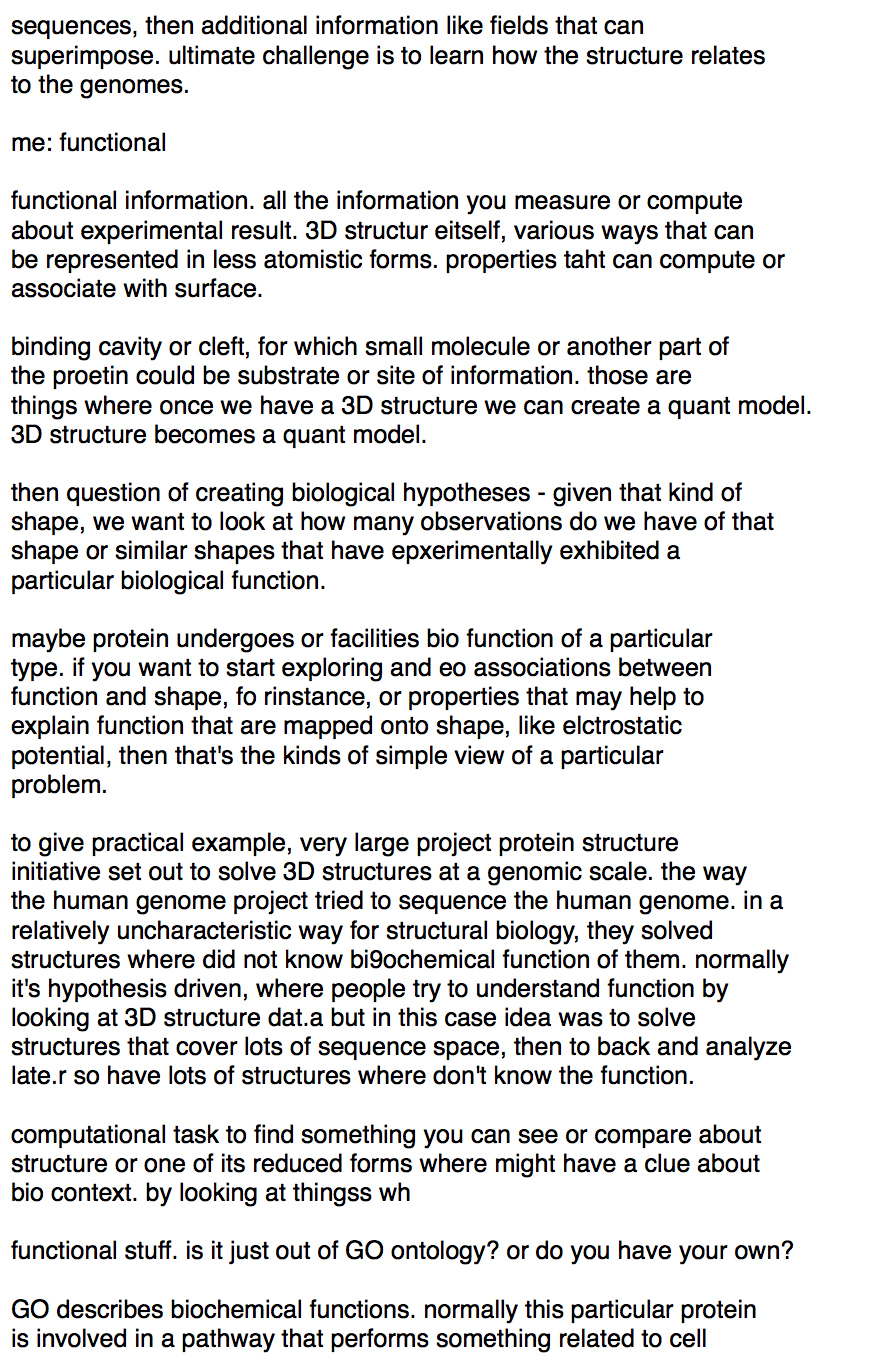
\includegraphics[width=.90\textwidth]{figures/sup_jwbnotes}} 
    \caption
    [
        An example of an interview transcript.
    ]
    {
        An example of an interview transcript (Analyst~\ref{drvistasks:analyst:JWB}).
    }
    \label{fig:jwbnotes}
    \centering
\end{figure}

%-|-|-|-|-|-|-|-|-|-|-|-|-|-|-|-|-|-|-|-|-|-|-|-|-|-|-|-|-|-|-|-|-|-|-|-|-

%-|-|-|-|-|-|-|-|-|-|-|-|-|-|-|-|-|-|-|-|-|-|-|-|-|-|-|-|-|-|-|-|-|-|-|-|-

\begin{figure}
    \centering
    \fbox{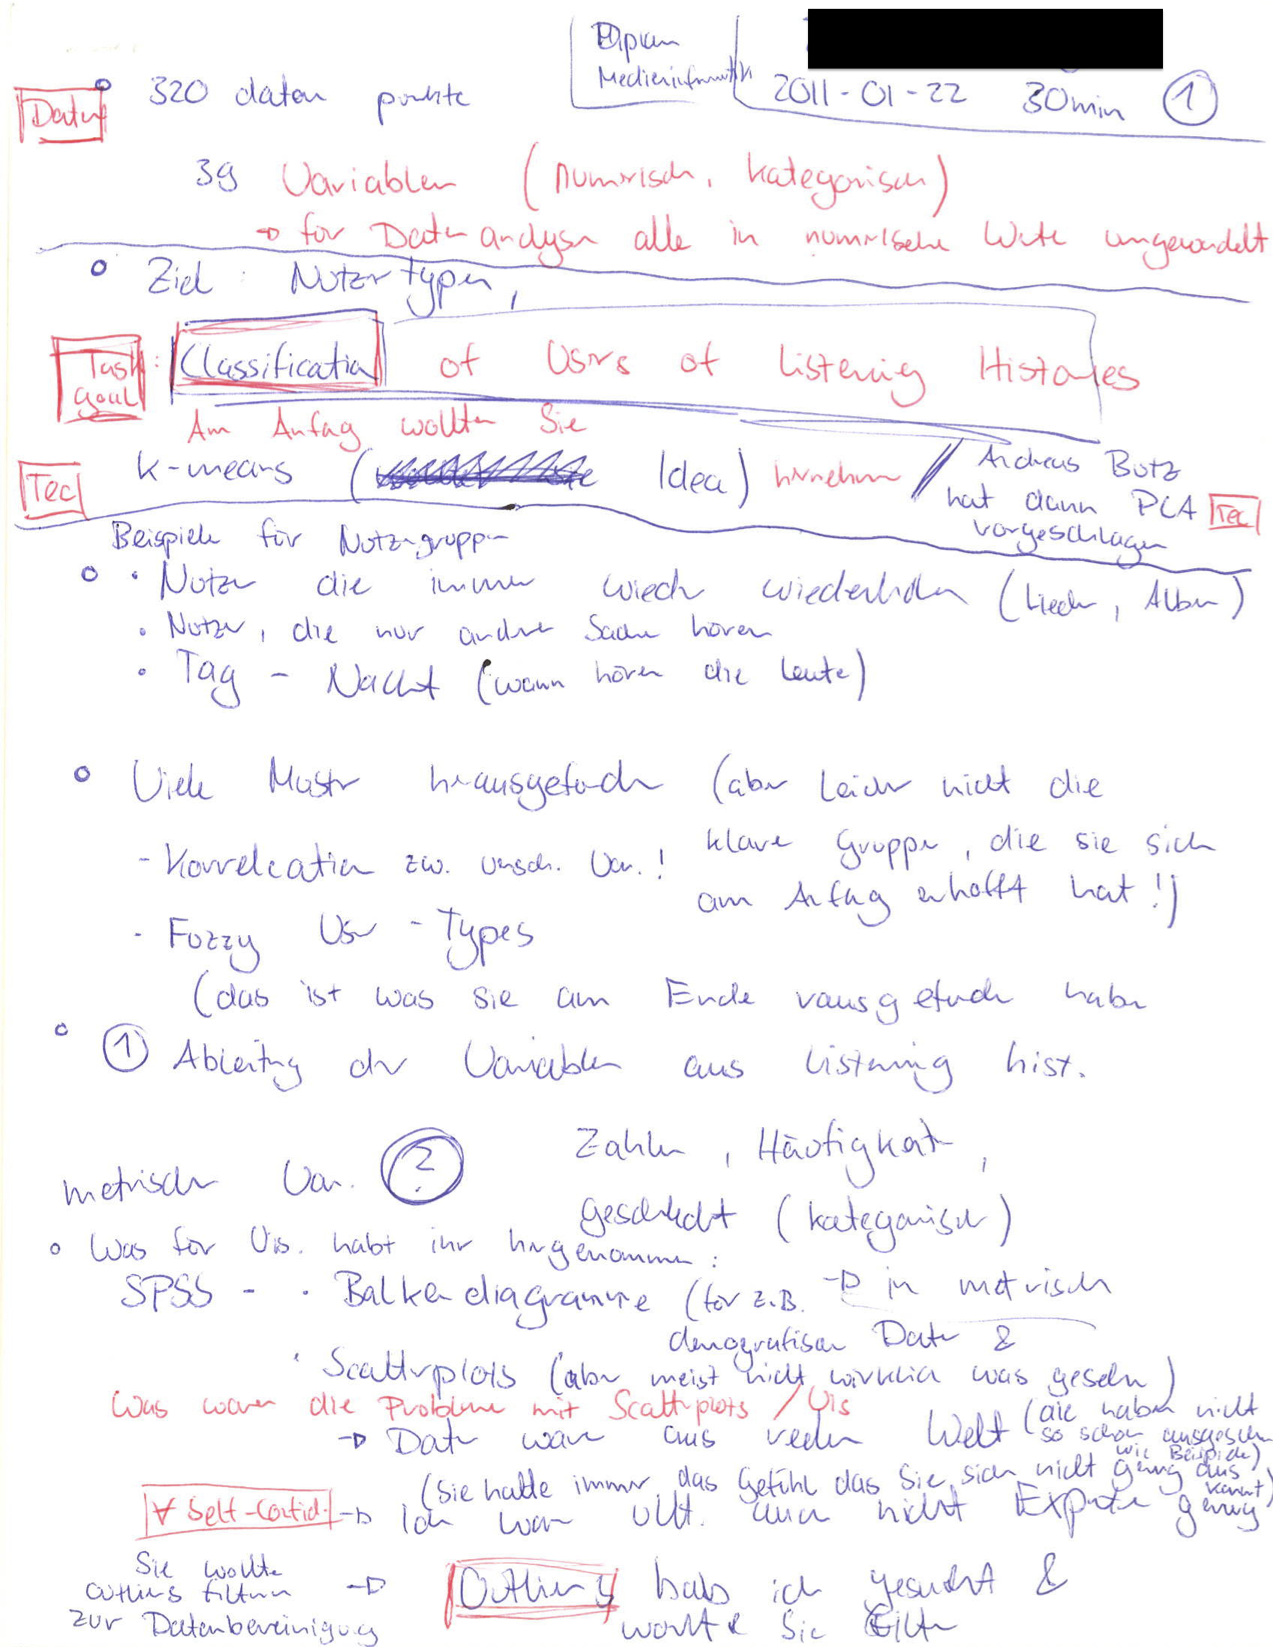
\includegraphics[width=.95\textwidth]{figures/sup_jbnotes}}
    \caption
    [
        An example of raw inter notes with post-hoc annotations.
    ]
    {
        Raw interview notes (blue ink) for Analyst~\ref{drvistasks:analyst:JB}, with post-hoc open coding (red ink) to identify concepts.
    }
    \label{fig:jbnotes}
    \centering
\end{figure}

%-|-|-|-|-|-|-|-|-|-|-|-|-|-|-|-|-|-|-|-|-|-|-|-|-|-|-|-|-|-|-|-|-|-|-|-|-

%-|-|-|-|-|-|-|-|-|-|-|-|-|-|-|-|-|-|-|-|-|-|-|-|-|-|-|-|-|-|-|-|-|-|-|-|-

\begin{figure}
    \centering
    \fbox{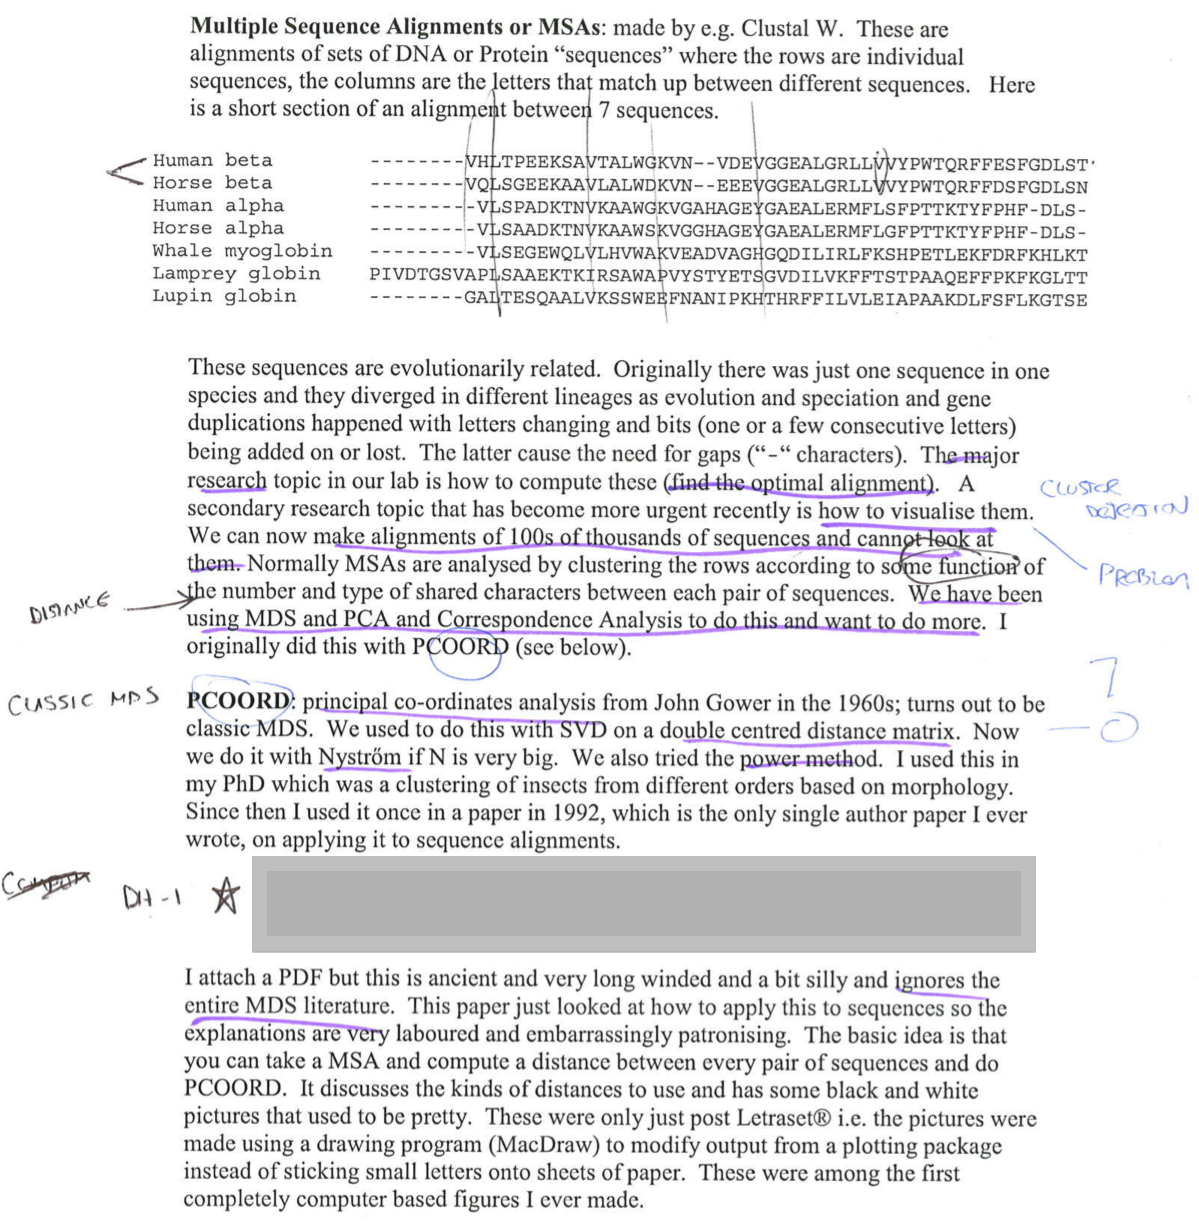
\includegraphics[width=.95\textwidth]{figures/sup_dhnotes}} 
    \caption
    [
        An example document sent to us by an analyst.
    ]
    {
        Document sent to us by Analyst~\ref{drvistasks:analyst:DH}, with post-hoc coding to identify concepts.
    }
    \label{fig:dhnotes}
    \centering
\end{figure}

%-|-|-|-|-|-|-|-|-|-|-|-|-|-|-|-|-|-|-|-|-|-|-|-|-|-|-|-|-|-|-|-|-|-|-|-|-

%-|-|-|-|-|-|-|-|-|-|-|-|-|-|-|-|-|-|-|-|-|-|-|-|-|-|-|-|-|-|-|-|-|-|-|-|-

\begin{figure}
    \centering
    \fbox{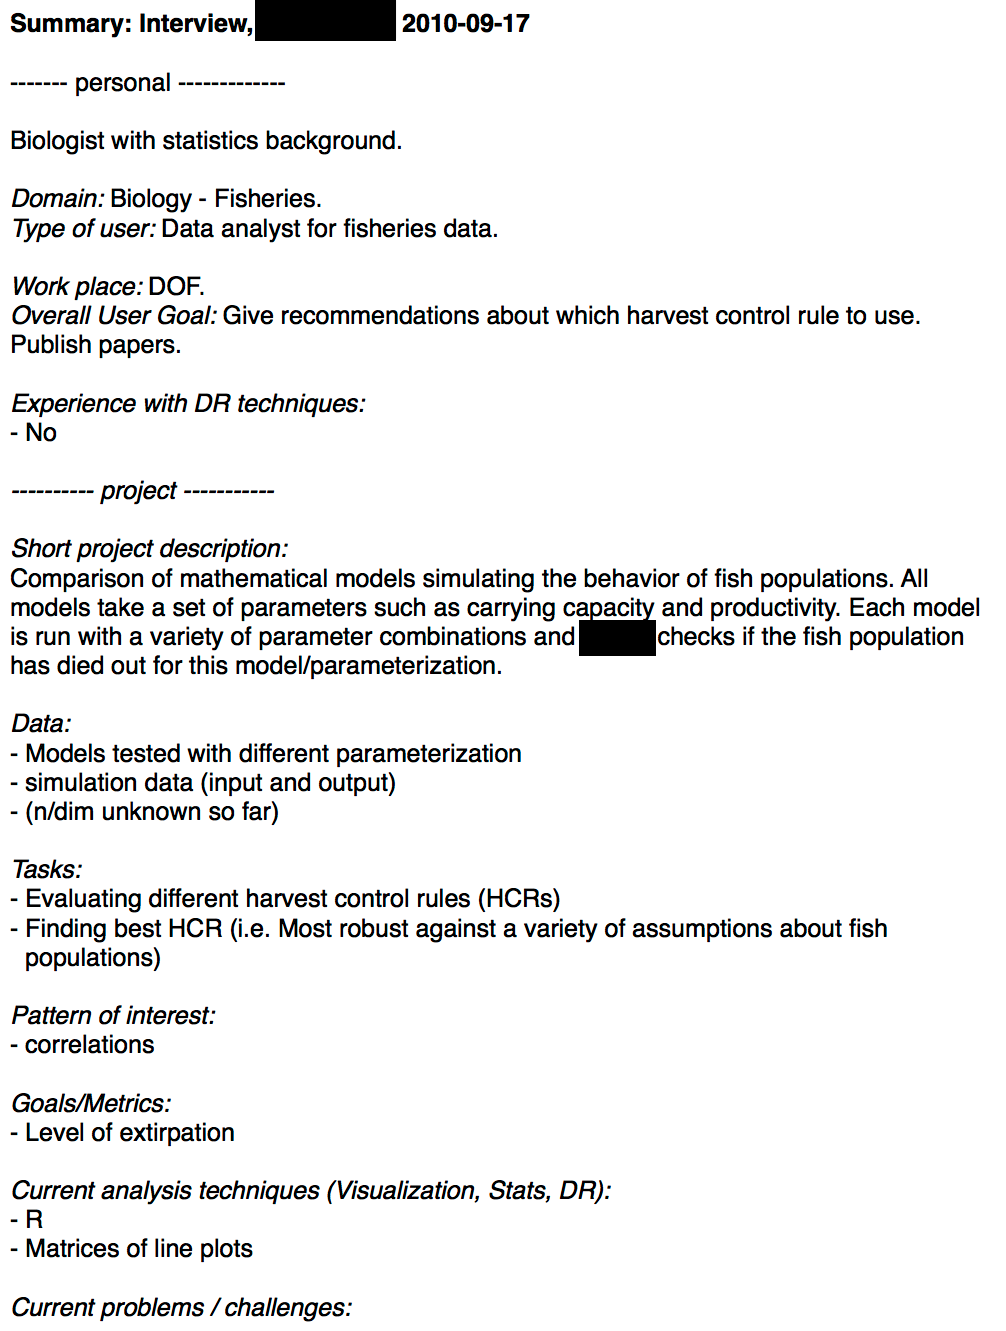
\includegraphics[width=.95\textwidth]{figures/sup_chsum}} 
    \caption
    [
        An early version of an analyst summary.
    ]
    {
        An early version for an analyst summary (Analyst~\ref{drvistasks:analyst:CH}), where the italicized headings reflect the result of focused coding to organizing concepts, properties, and dimensions. 
    }
    \label{fig:chsum}
    \centering
\end{figure}

%-|-|-|-|-|-|-|-|-|-|-|-|-|-|-|-|-|-|-|-|-|-|-|-|-|-|-|-|-|-|-|-|-|-|-|-|-

%-|-|-|-|-|-|-|-|-|-|-|-|-|-|-|-|-|-|-|-|-|-|-|-|-|-|-|-|-|-|-|-|-|-|-|-|-

\begin{figure}
    \centering
    \fbox{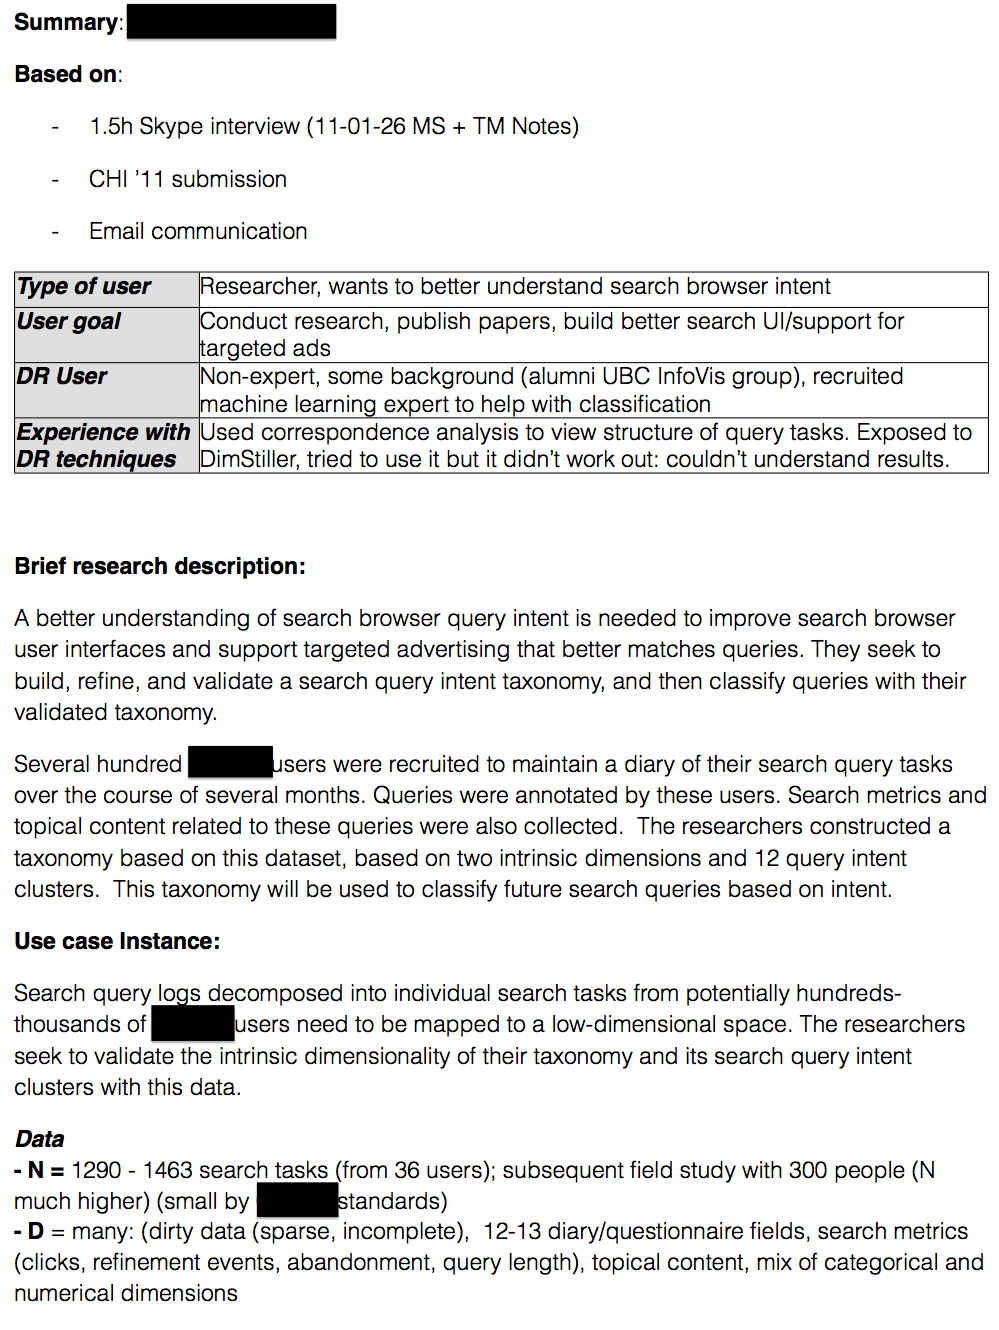
\includegraphics[width=.95\textwidth]{figures/sup_hlsum}}
    \caption
    [
        A later version of an analyst summary.
    ]
    {
        A later version of an analyst summary (Analyst~\ref{drvistasks:analyst:HL}), where the bold headings reflect our focused coding: concepts, properties, and dimensions. 
    }
    \label{fig:hlsum}
    \centering
\end{figure}

%-|-|-|-|-|-|-|-|-|-|-|-|-|-|-|-|-|-|-|-|-|-|-|-|-|-|-|-|-|-|-|-|-|-|-|-|-

%-|-|-|-|-|-|-|-|-|-|-|-|-|-|-|-|-|-|-|-|-|-|-|-|-|-|-|-|-|-|-|-|-|-|-|-|-

\begin{table}
    \centering
    \fbox{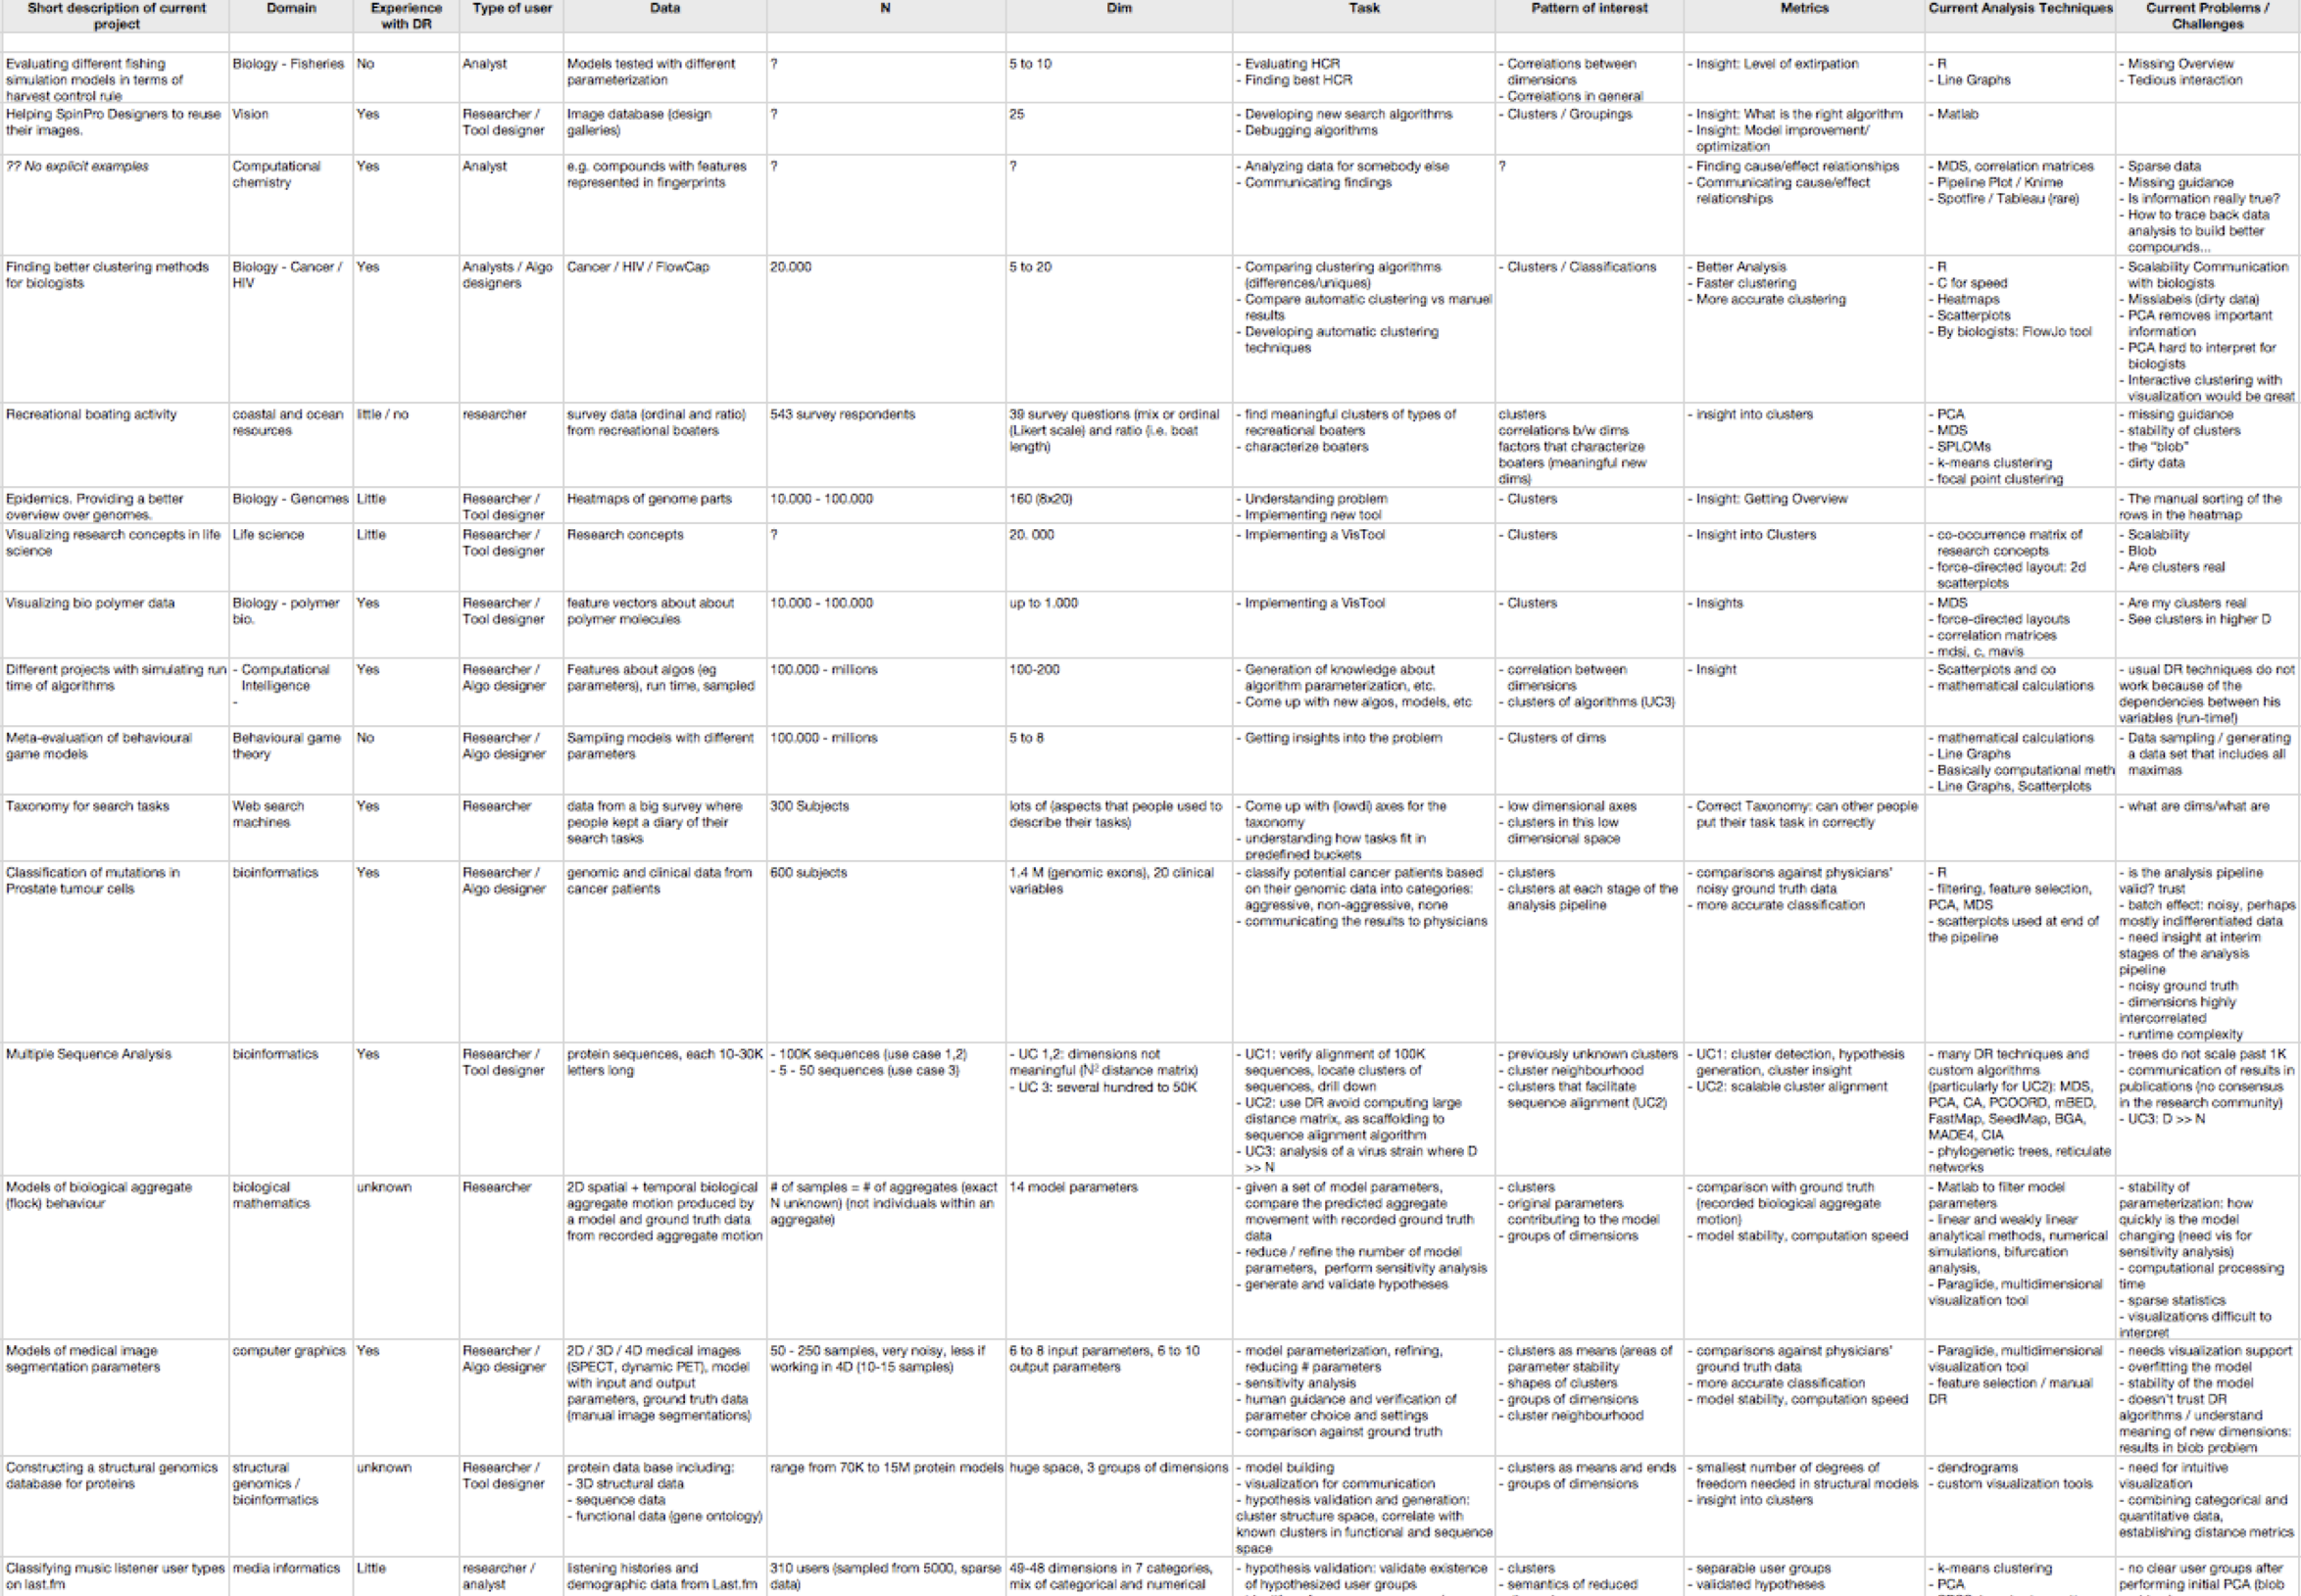
\includegraphics[width=0.975\textwidth]{figures/sup_sumtab}} 
    \caption
    [
        Establishing conceptual relationships across summaries.
    ]
    {
        Establishing conceptual relationships across summaries.
    }
    \label{table:sum-tab}
    \centering
\end{table}

%-|-|-|-|-|-|-|-|-|-|-|-|-|-|-|-|-|-|-|-|-|-|-|-|-|-|-|-|-|-|-|-|-|-|-|-|-

%-|-|-|-|-|-|-|-|-|-|-|-|-|-|-|-|-|-|-|-|-|-|-|-|-|-|-|-|-|-|-|-|-|-|-|-|-

\begin{table}
    \centering
    \fbox{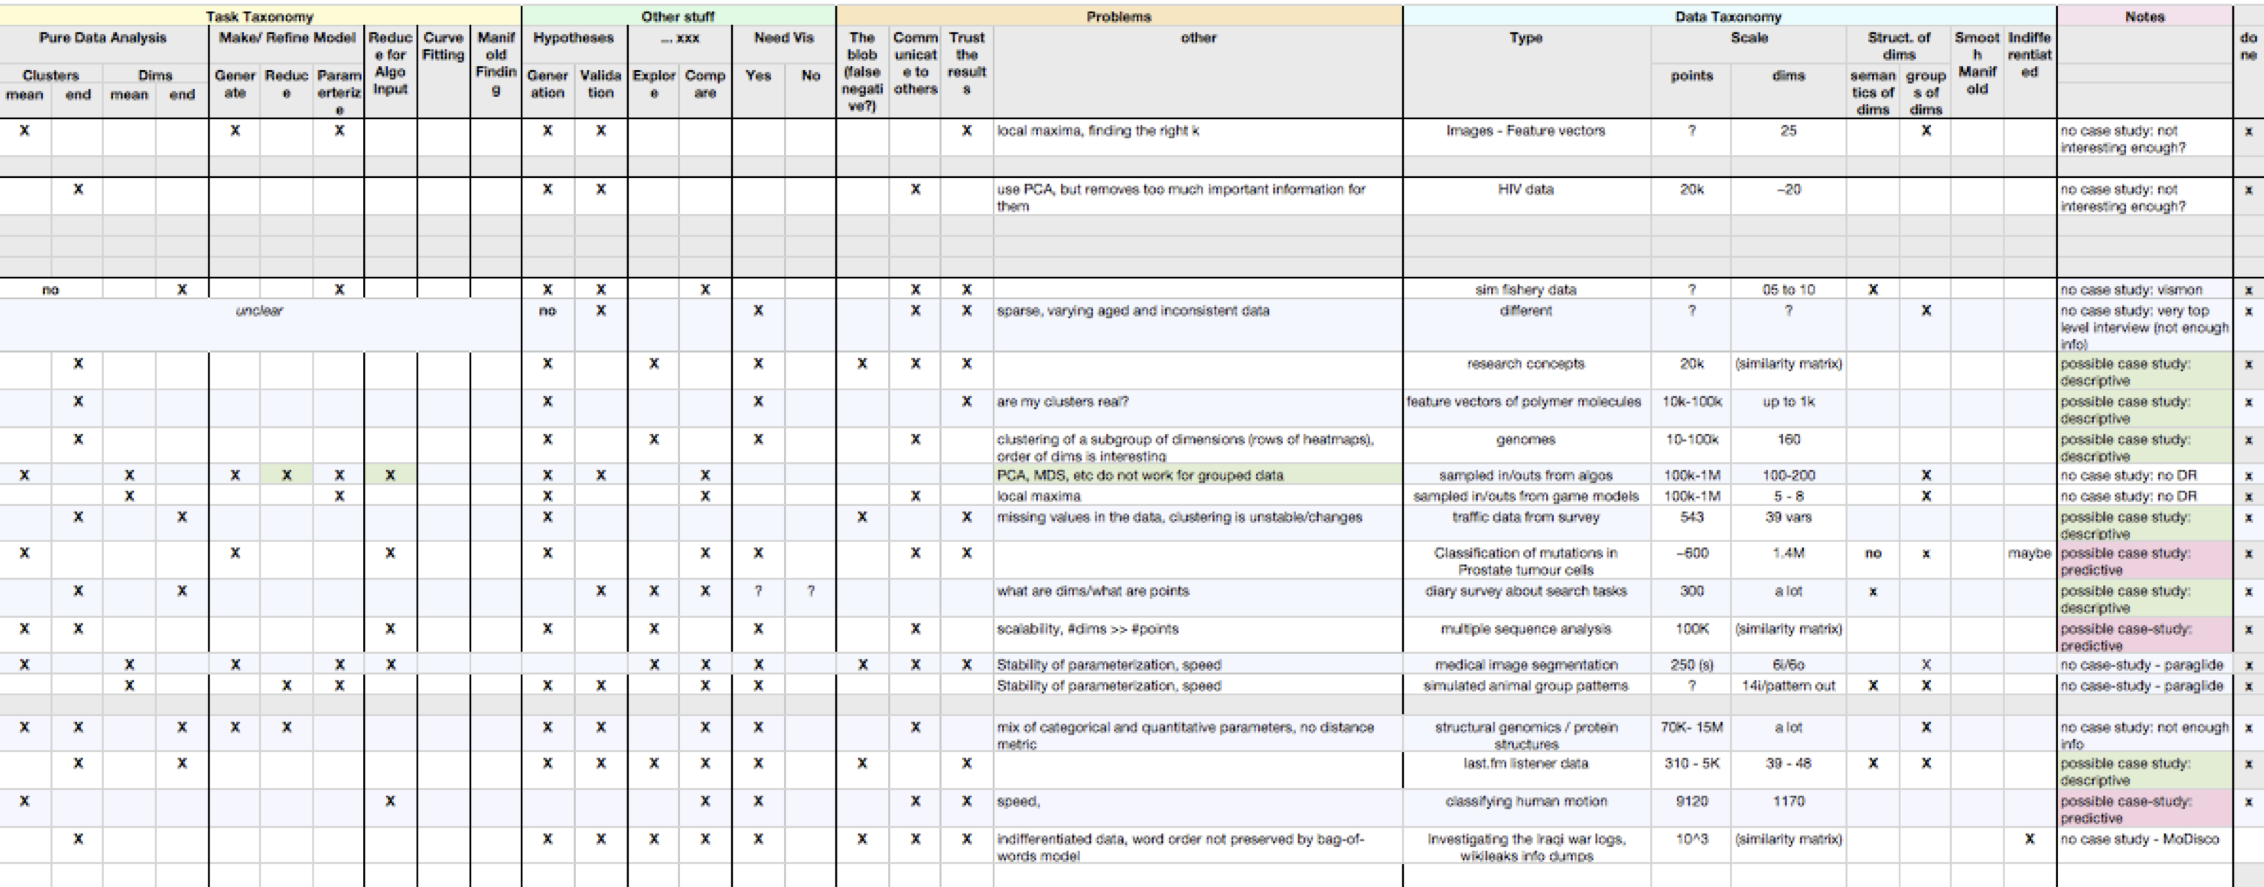
\includegraphics[width=0.975\textwidth]{figures/sup_sumtab2}} 
    \caption
    [
        Establishing conceptual relationships across summaries (continued).
    ]
    {
        Establishing conceptual relationships across summaries (continued).
    }
    \label{table:sum-tab-2}
    \centering
\end{table}

%-|-|-|-|-|-|-|-|-|-|-|-|-|-|-|-|-|-|-|-|-|-|-|-|-|-|-|-|-|-|-|-|-|-|-|-|-

%-|-|-|-|-|-|-|-|-|-|-|-|-|-|-|-|-|-|-|-|-|-|-|-|-|-|-|-|-|-|-|-|-|-|-|-|-

\begin{table}
    \centering
    \fbox{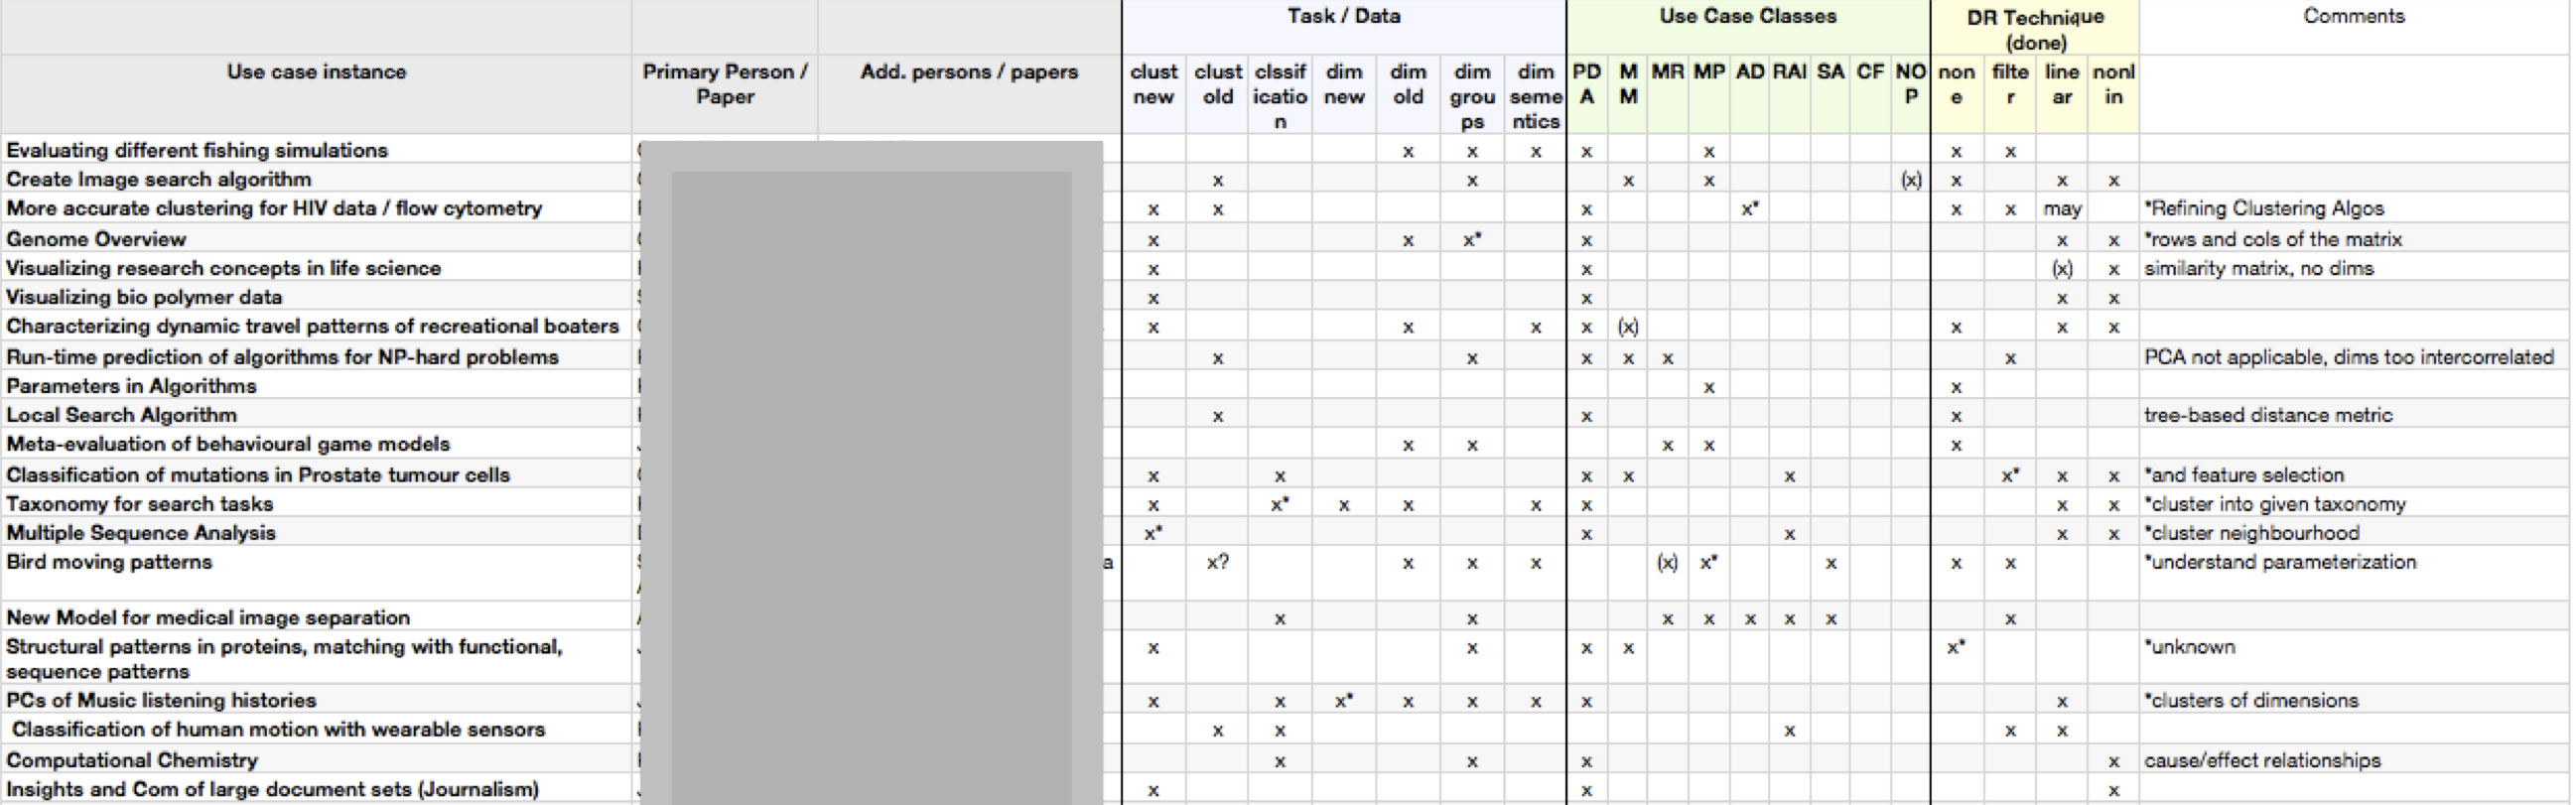
\includegraphics[width=0.975\textwidth]{figures/sup_sumtab3}}
    \caption
    [
        Establishing conceptual relationships across summaries (continued).
    ]
    {
        Establishing conceptual relationships across summaries (continued).
    }
    \label{table:sum-tab-3}
    \centering
\end{table}

%-|-|-|-|-|-|-|-|-|-|-|-|-|-|-|-|-|-|-|-|-|-|-|-|-|-|-|-|-|-|-|-|-|-|-|-|-

%-|-|-|-|-|-|-|-|-|-|-|-|-|-|-|-|-|-|-|-|-|-|-|-|-|-|-|-|-|-|-|-|-|-|-|-|-

\begin{table}
    \centering
    \fbox{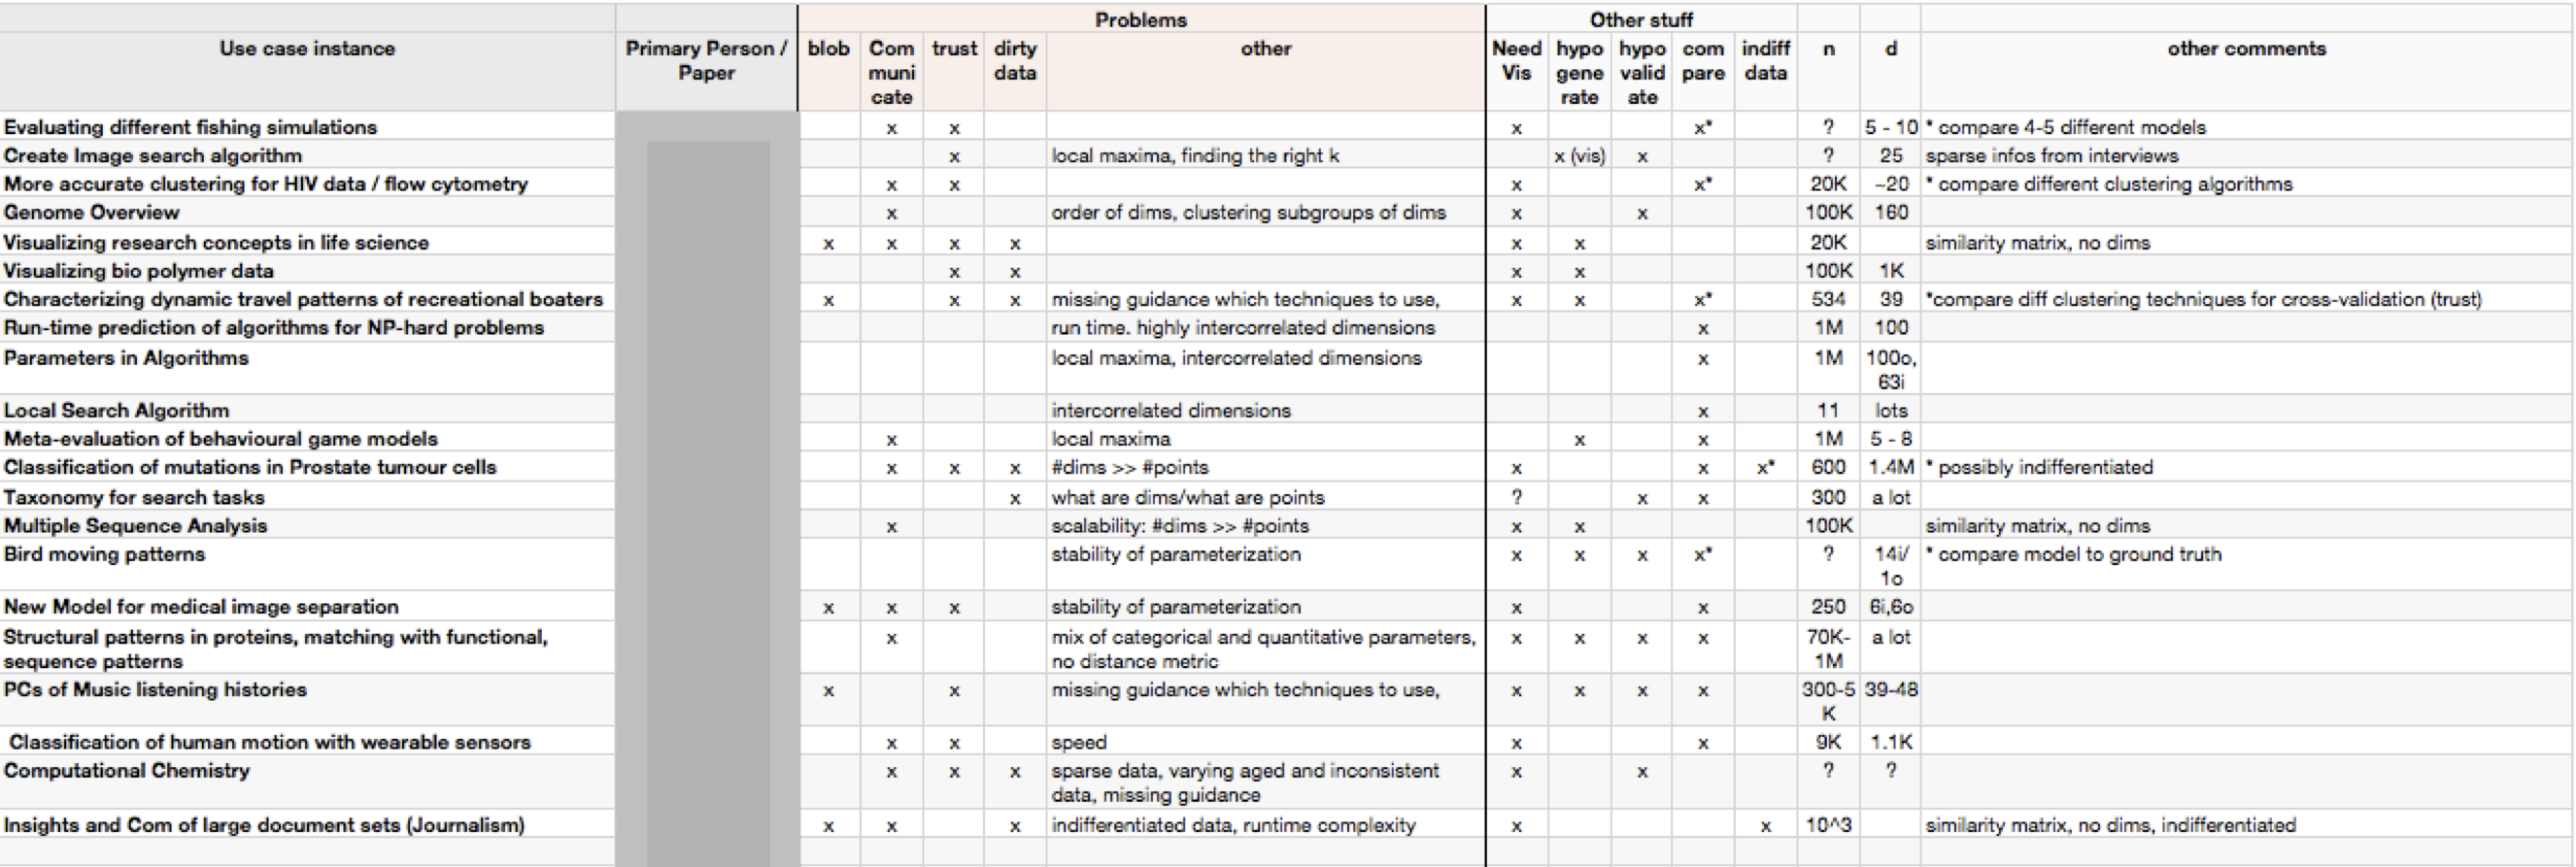
\includegraphics[width=0.975\textwidth]{figures/sup_sumtab4}}
    \caption
    [
        Establishing conceptual relationships across summaries (continued).
    ]
    {
        Establishing conceptual relationships across summaries (continued).
    }
    \label{table:sum-tab-4}
    \centering
\end{table}

%-|-|-|-|-|-|-|-|-|-|-|-|-|-|-|-|-|-|-|-|-|-|-|-|-|-|-|-|-|-|-|-|-|-|-|-|-

% \autoref{table:sum-tab-5} represents the result of categorizing analysts' outcomes as as {\it happy}, {\it struggling}, or {\it failing}.

% %-|-|-|-|-|-|-|-|-|-|-|-|-|-|-|-|-|-|-|-|-|-|-|-|-|-|-|-|-|-|-|-|-|-|-|-|-

% \begin{figure}
%     \centering
%     \fbox{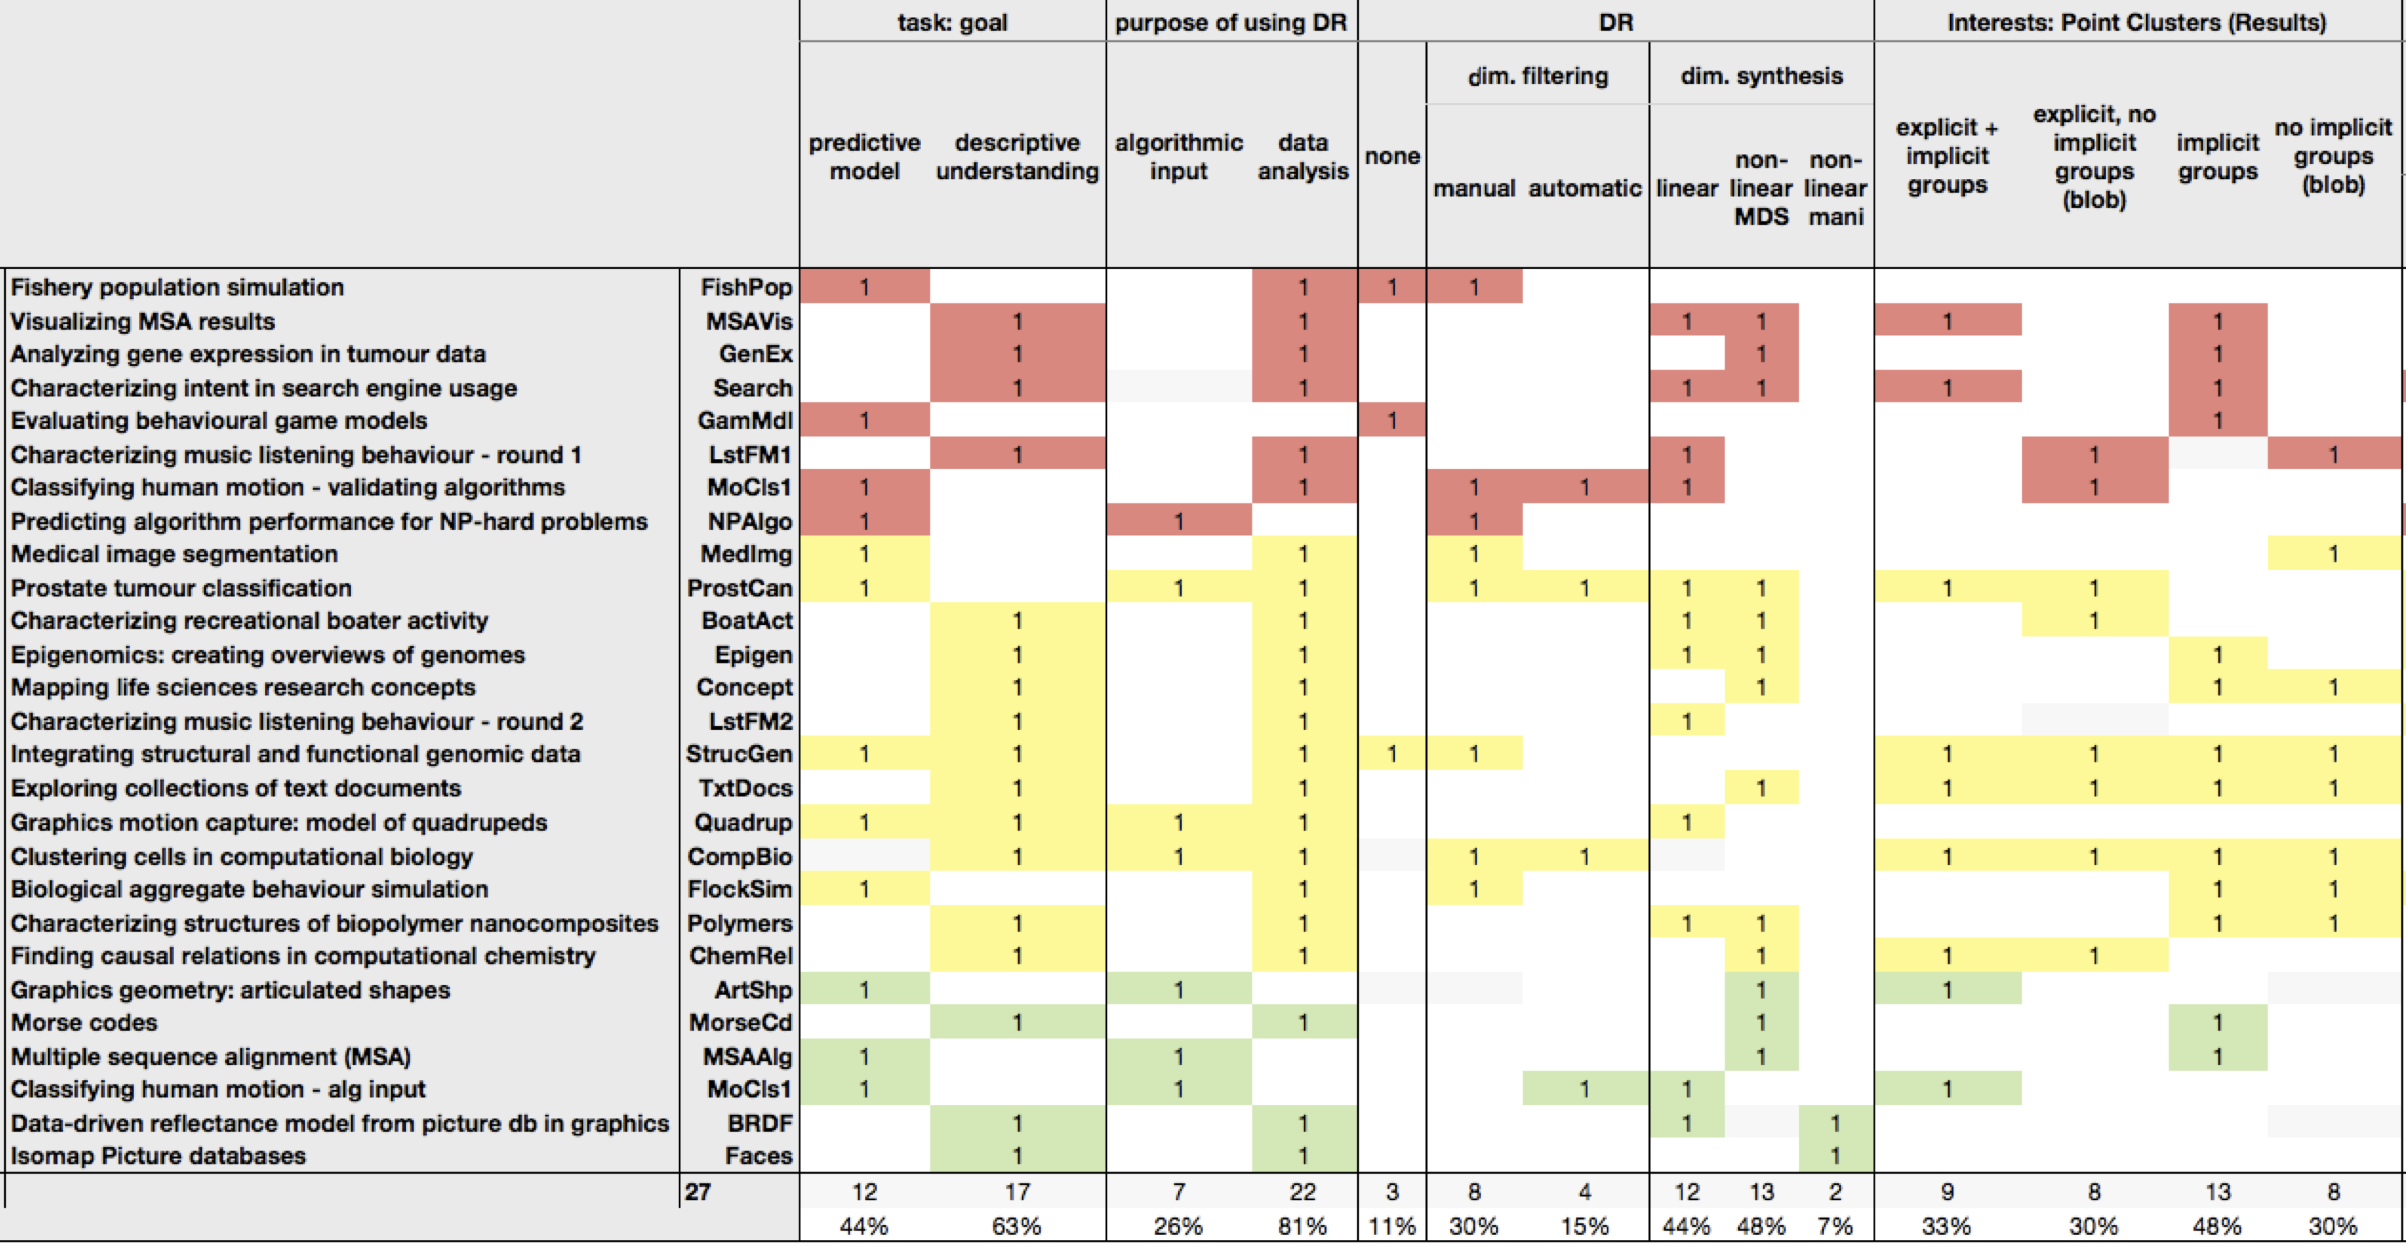
\includegraphics[width=.95\textwidth]{figures/sup_sumtab5}}
%     \caption
%     [
%         Classifying the analysts' outcomes.
%     ]
%     {
%         Classifying the analysts' outcomes: {\it happy} (green), {\it struggling} (yellow), or {\it failing} (red).
%     }
%     \label{table:sum-tab-5}
%     \centering
% \end{figure}

% %-|-|-|-|-|-|-|-|-|-|-|-|-|-|-|-|-|-|-|-|-|-|-|-|-|-|-|-|-|-|-|-|-|-|-|-|-


%-|-|-|-|-|-|-|-|-|-|-|-|-|-|-|-|-|-|-|-|-|-|-|-|-|-|-|-|-|-|-|-|-|-|-|-|-

% \begin{sidewaysfigure}
%     \centering
%     \fbox{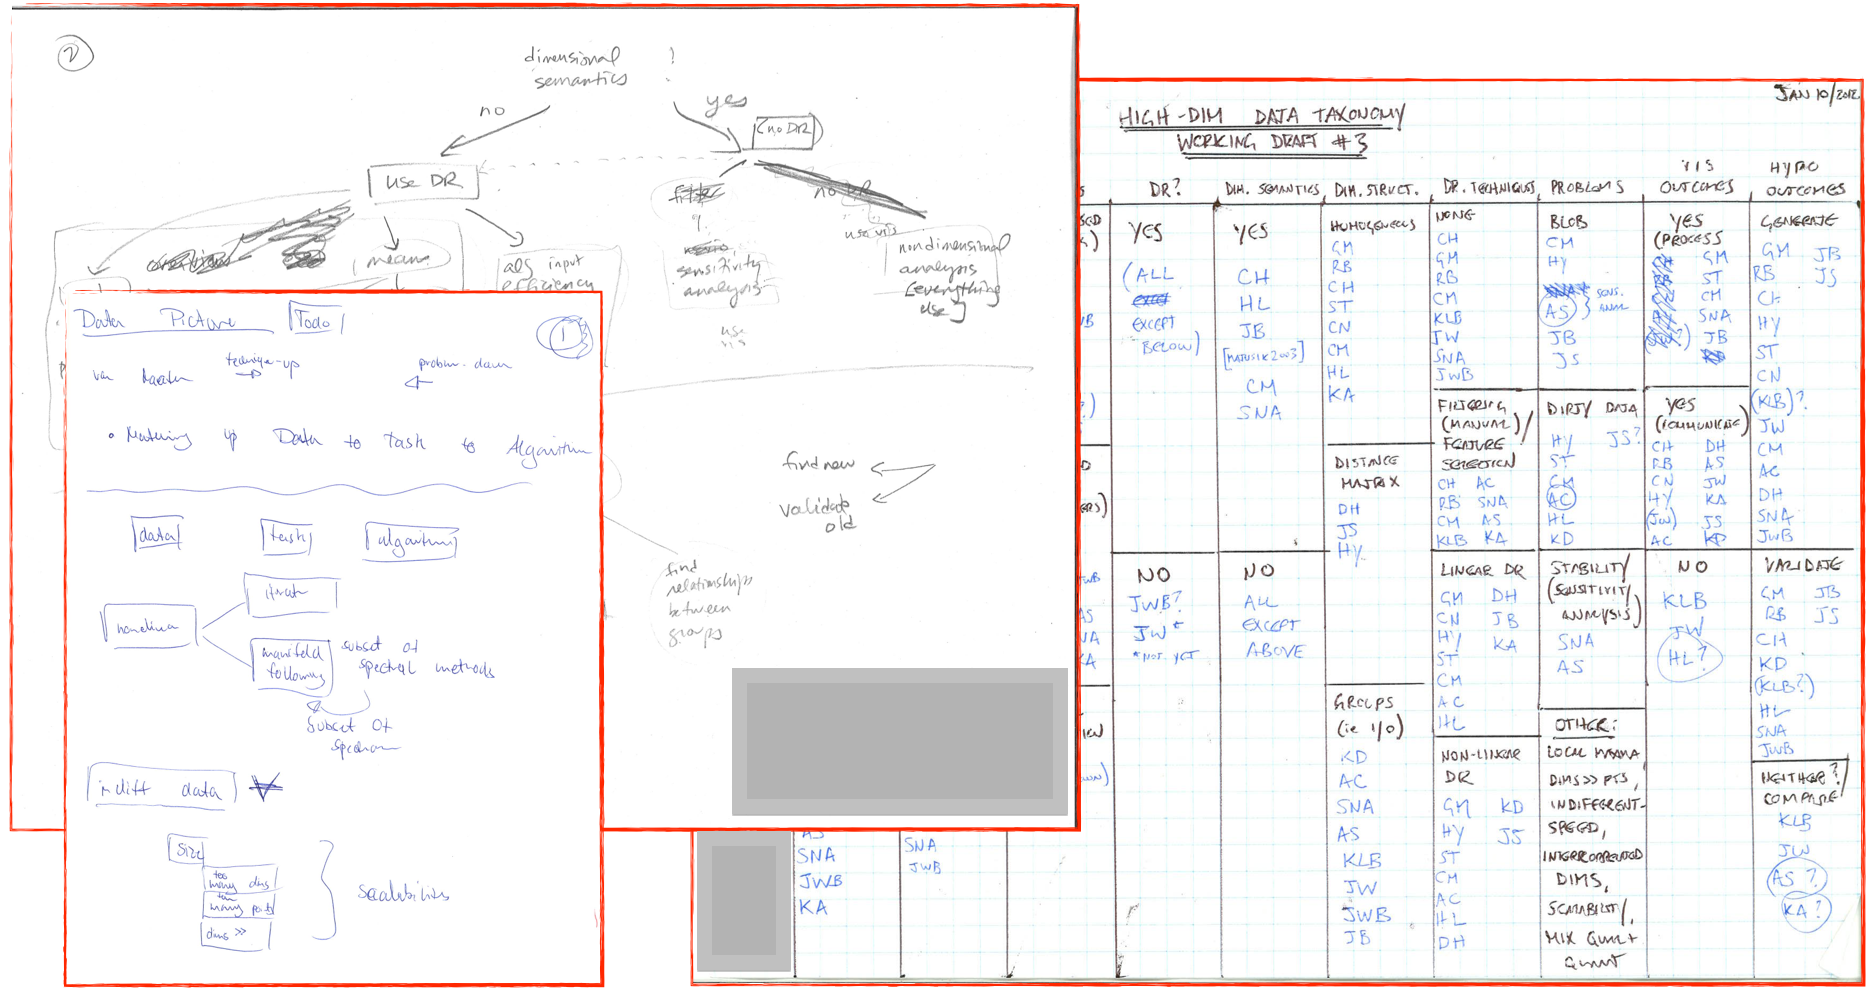
\includegraphics[width=.95\textwidth]{figures/sup_memos}}
%     \caption
%     [
%         Examples of memos and theorizing.
%     ]
%     {
%         Examples of memos and ongoing theorizing occurring during the course of data analysis. 
%     }
%     \label{fig:memos}
%     \centering
% \end{sidewaysfigure}

%-|-|-|-|-|-|-|-|-|-|-|-|-|-|-|-|-|-|-|-|-|-|-|-|-|-|-|-|-|-|-|-|-|-|-|-|-

%-------------------------------------------------------------------------
%-------------------------------------------------------------------------

\section{Previous Interpretations of Findings}
\label{app:drvistasks:previous-interpretations}

%-------------------------------------------------------------------------
%-------------------------------------------------------------------------

The initial interpretation of our findings~\cite{Sedlmair2012b} (summarized in \autoref{fig:dritw-taxonomy-1}) classifies people who use \ac{DR}\index{dimensionality reduction (DR)}, \ac{DR}\index{dimensionality reduction (DR)} techniques, tasks, and the challenges faced by these people.
Unlike the analysis presented in \autoref{ch:drvistasks}, we did not exclude cases in which visualization did not occur, nor did we exclude cases in which {\it dimensional filtering}\index{dimensionality reduction (DR)!dimensional filtering} techniques (\eg\cite{Johansson2009,Yang2003}) were used\footnote{In \autoref{ch:drvistasks}, we concentrate on tasks\index{task} relating to visualizing the results of {\it dimensional synthesis} techniques, such as \ac{PCA} or \ac{MDS}.}.
Our findings are summarized according to this classification in \autoref{table:dritw-table-1}.
A revised interpretation of our findings\footnote{Reproduced below in \autoref{app:drvistasks:dritw}.} focuses primarily on tasks\index{task} relating to \ac{DR}\index{dimensionality reduction (DR)} (\autoref{fig:dritw-taxonomy-2}), with less emphasis on challenges.
Our findings are summarized according to this classification in \autoref{table:dritw-table-2}.
% Finally, the interpretation of our findings presented in \autoref{ch:drvistasks} is the result of a concentrated focus on tasks relating to the visualization of dimensionally reduced data and the use of {\it dimensional synthesis} \ac{DR} techniques in particular, which excludes tasks that do not involve visualization or the use of other \ac{DR} approaches, such as {\it dimensional filtering}.

%-|-|-|-|-|-|-|-|-|-|-|-|-|-|-|-|-|-|-|-|-|-|-|-|-|-|-|-|-|-|-|-|-|-|-|-|-

\begin{figure}
    \centering
    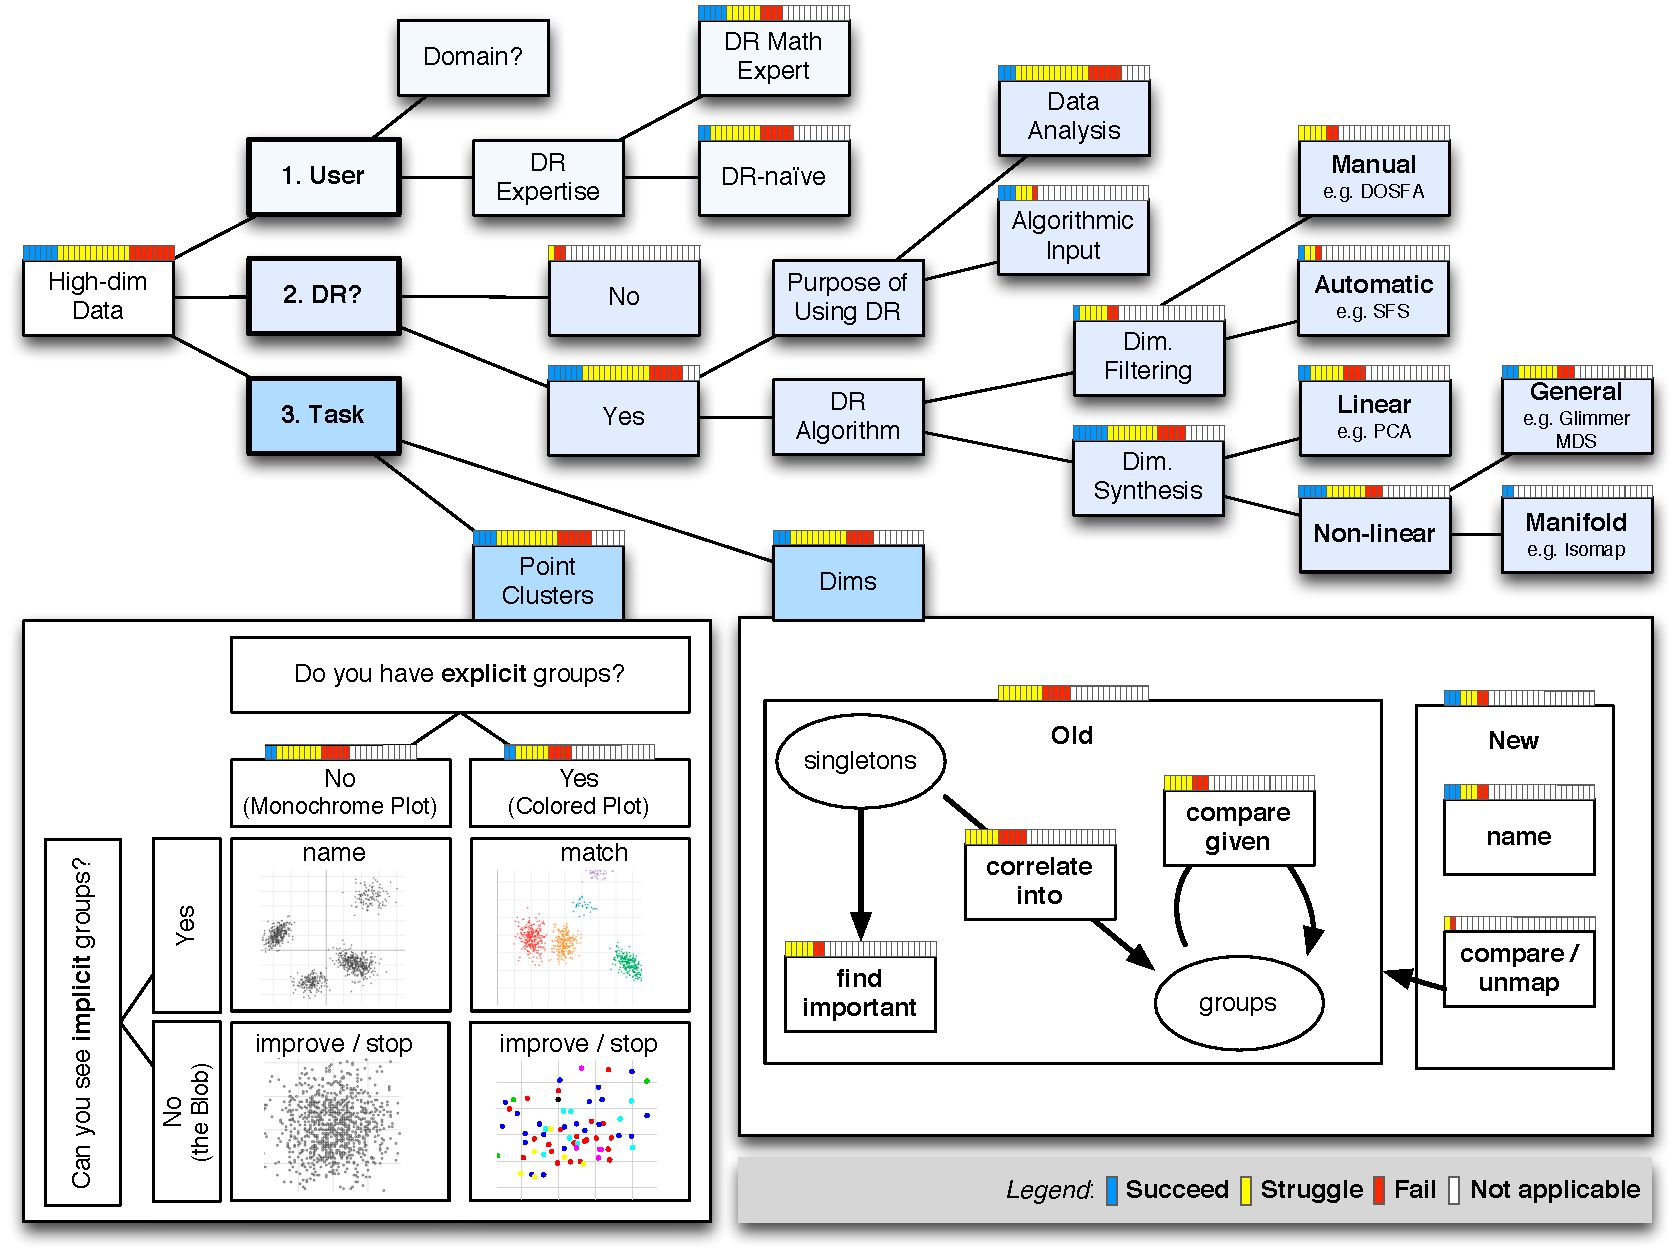
\includegraphics[width=\textwidth]{figures/dritw-taxonomy-1.pdf}
    \caption
    [
        Our preliminary classification of people who use \ac{DR}, \ac{DR} techniques, and tasks.
    ]
    {
        Our preliminary classification of high-dimensional data analysis in terms of people who use \ac{DR}, \ac{DR} techniques, and tasks~\cite{Sedlmair2012b}. References: DOSFA (Dimension Ordering, Spacing and Filtering Approach)~\cite{Yang2003}, \ac{SFS}~\cite{Jain2000}, \ac{PCA}~\cite{Jolliffe2002}, Isomap~\cite{Tenenbaum2000}, Glimmer \ac{MDS}~\cite{Ingram2009}.  
    }
    \label{fig:dritw-taxonomy-1}
    \centering
\end{figure}

%-|-|-|-|-|-|-|-|-|-|-|-|-|-|-|-|-|-|-|-|-|-|-|-|-|-|-|-|-|-|-|-|-|-|-|-|-

%-|-|-|-|-|-|-|-|-|-|-|-|-|-|-|-|-|-|-|-|-|-|-|-|-|-|-|-|-|-|-|-|-|-|-|-|-

\begin{table}
    \centering
    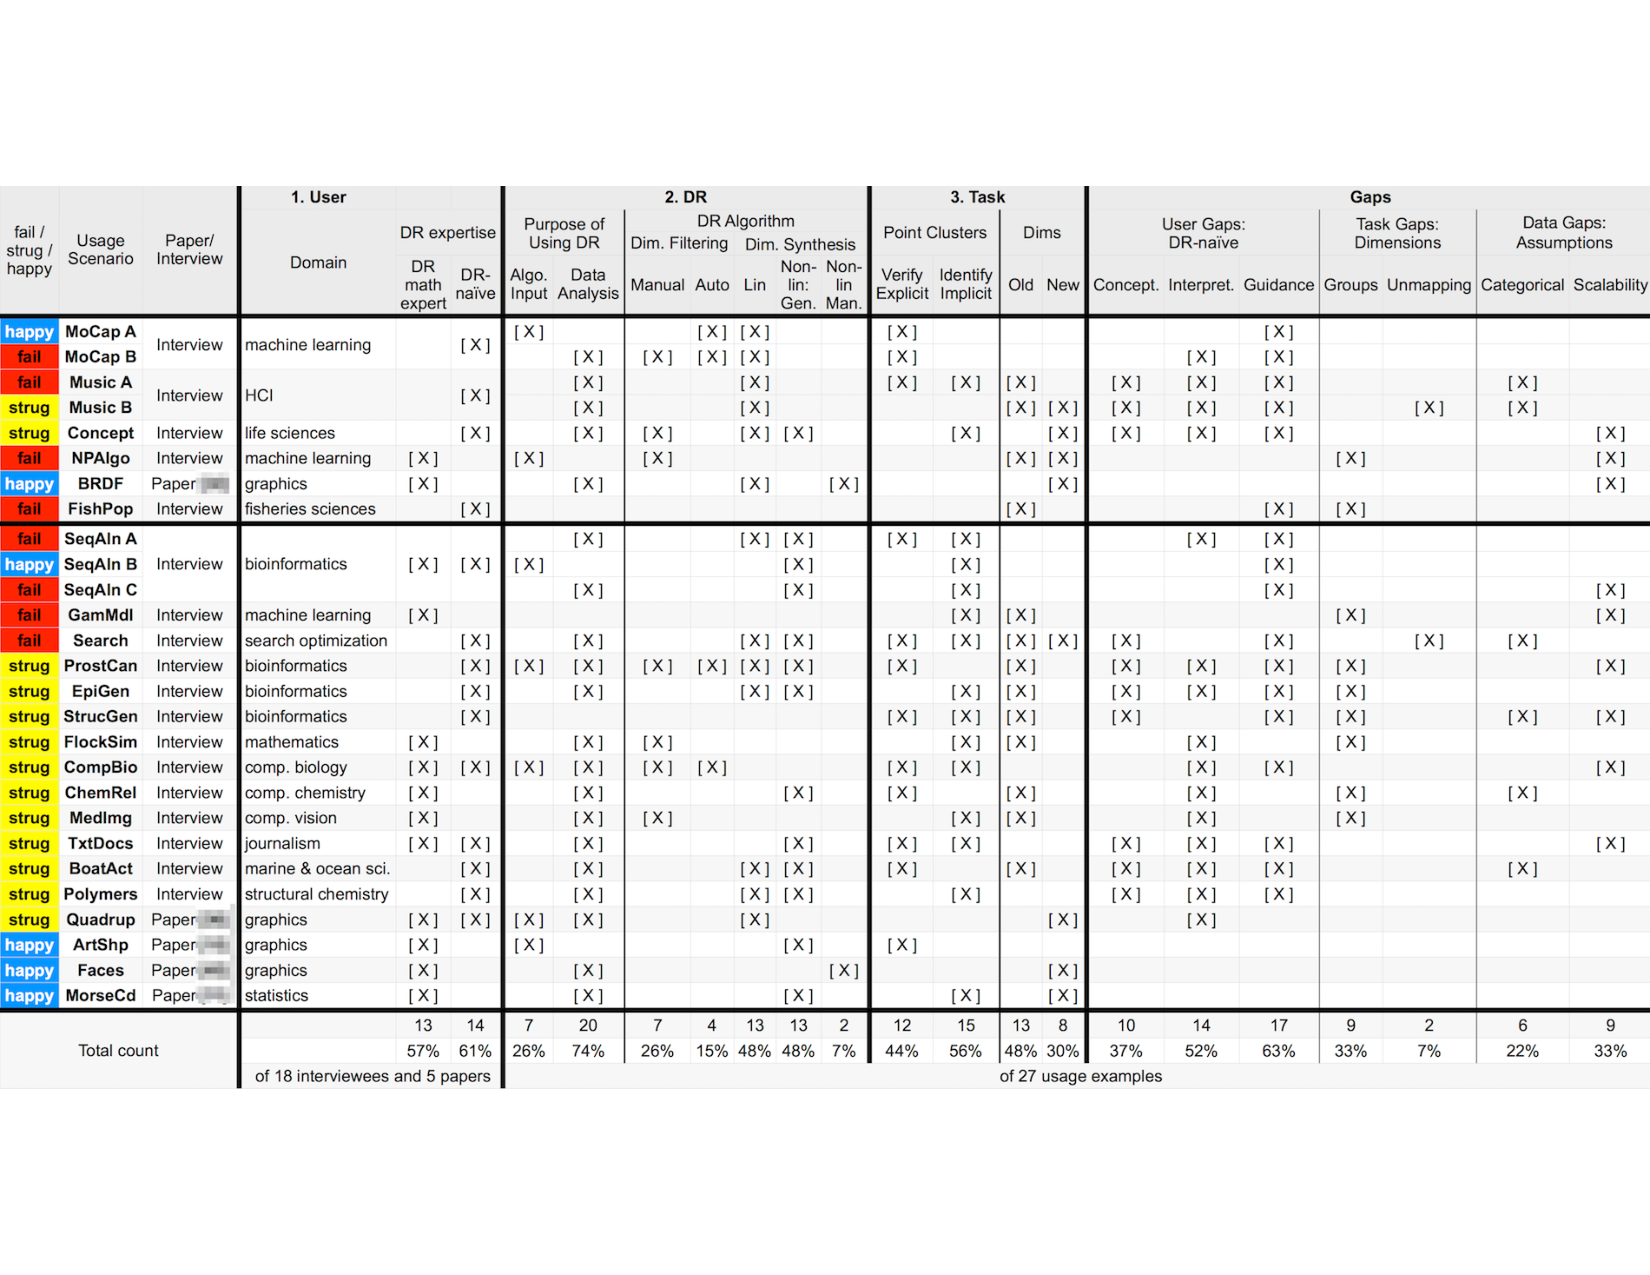
\includegraphics[width=\textwidth]{figures/dritw-table-1.pdf}
    \caption
    [
        Usage examples described using our preliminary classification of people who use \ac{DR}, \ac{DR} techniques, and tasks. 
    ]
    {
        Usage examples described using our preliminary classification of people who use \ac{DR}, \ac{DR} techniques, tasks, and gaps. For a description of the gaps, see our technical report~\cite{Sedlmair2012b}. Paper references: {\sc BRDF}~\cite{Matusik2003}, {\sc ArtShp}~\cite{Bronstein2006}, {\sc Faces}~\cite{Tenenbaum2000}, {\sc MorseCd}~\cite{Buja2002}. The usage example abbreviations correspond to analyst ID numbers listed in \autoref{tab:interviews}. 
    }
    \label{table:dritw-table-1}
    \centering
\end{table}

%-|-|-|-|-|-|-|-|-|-|-|-|-|-|-|-|-|-|-|-|-|-|-|-|-|-|-|-|-|-|-|-|-|-|-|-|-

%-------------------------------------------------------------------------
%-------------------------------------------------------------------------

\section{Dimensionality Reduction in the Wild}
\label{app:drvistasks:dritw}

%-------------------------------------------------------------------------
%-------------------------------------------------------------------------

\footnote{This section is a slightly modified version of our unpublished manuscript {\it Dimensionality Reduction in the Wild} by Michael Sedlmair, Matthew Brehmer, Stephen Ingram, and Tamara Munzner (2013).} In this manuscript, we contribute the first systematic and broad analysis of dimensionality reduction (DR) usage conducted ``in the wild''\index{evaluation!in the wild}, by observing the usage patterns of real data analysts, along with their needs and problems. 
We present the results of a two-year qualitative research endeavor, in which we iteratively collected and analyzed a rich corpus of data. 
We interviewed nineteen data analysts from ten different domains and selected five papers describing data analysis using \ac{DR}\index{dimensionality reduction (DR)}, deriving twenty-seven real-world usage examples in total.
Grounded in this data, the main contribution of this paper is a classification of tasks\index{task} that relate to high dimensional data analysis and the use of \ac{DR}\index{dimensionality reduction (DR)}. 
Its high-level structure differentiates between abstract tasks\index{task!task abstraction} related to the visual analysis of scatterplots\index{visual encoding!scatterplot} versus of dimensions, in contrast to reducing dimensionality for downstream usage by completely automatic algorithms\index{algorithms}. 
%-------------------------------------------------------------------------

\subsection{Introduction}
\label{app:drvistasks:dritw:introduction}

%-------------------------------------------------------------------------

\begin{sloppypar}
\ac{DR}\index{dimensionality reduction (DR)} is the process of reducing a high- dimensional dataset to a low-dimensional visual encoding\index{visual encoding} that retains most of its important structure. 
It has been an active research area throughout several decades and across many domains, from its origins in psychology~\cite{Torgerson1952,Young1938} through statistics~\cite{Buja2002} to machine learning\index{machine learning}
~\cite{Belkin2001,Guyon2003,Jain2000,Tenenbaum2000,VanderMaaten2008} and visualization
~\cite{Ingram2009,Johansson2009,Yang2003}.
\end{sloppypar}

The \ac{DR}\index{dimensionality reduction (DR)} literature is heavily focused on mathematical and algorithmic\index{algorithms} descriptions of new techniques and their characterization based on algorithmic\index{algorithms} properties \cite{Cunningham2008,France2011,Guyon2003,Jain2000,VanderMaaten2009,Witten2011}. 
In recent years, the visualization community has increasingly focused on understanding the analysts' perspective, as part of the quest for visualization design and evaluation\index{evaluation} that reflects real needs and activities~\cite{Kandel2012,Kang2011,Munzner2009}.
However, almost no work has considered \ac{DR}\index{dimensionality reduction (DR)} from a such human-centered perspective.
Many questions about how \ac{DR}\index{dimensionality reduction (DR)} is actually used {\it in the wild}\index{evaluation!in the wild}, in real world settings with real datasets, remain open: when do those with high-dimensional data\index{high-dimensional data} use \ac{DR}\index{dimensionality reduction (DR)} techniques? 
What are their tasks\index{task} and goals, considered at an abstract level\index{task!task abstraction}? 
Which \ac{DR}\index{dimensionality reduction (DR)} techniques do they use and how do they use them? 
How well do their real datasets match up with common benchmarks? Understanding these questions can guide both technique-driven work such as further algorithmic\index{algorithms} development, and problem-driven work such as design studies\index{design studies}. 

With these questions in mind, we engaged in a two-year qualitative research project based on semi-structured interviews with nineteen data analysts from ten application domains, followed by extensive analysis based on iterative coding\index{coding (qualitative data analysis)}. 
We present the results as a classification of abstract tasks\index{task!task abstraction} that provide a framework for understanding how, when, and why analysts might use \ac{DR}\index{dimensionality reduction (DR)}. 
Our task\index{task} classification has three categories at the highest level: {\it learning about dimensions}, {\it seeing clusters}, and reducing dimensionality for the purpose of {\it algorithmic input}\index{algorithms!algorithmic input}. 
We focus on the former two as visual data exploration tasks\index{task} are particularly important for the visualization community, rather than the latter usage that is common practice in completely automatic analysis, as in the machine learning\index{machine learning} community~\cite{Murphy2012}.

We also relate our observations of analysts' in-the-wild practices to the technical \ac{DR}\index{dimensionality reduction (DR)} literature, providing a synthesis overview that is accessible to the visualization community. 
We also provide an analysis of the relationships between the tasks\index{task} in our classification and benchmark datasets common in \ac{DR}\index{dimensionality reduction (DR)} algorithm development and usage, and discuss challenges encountered by the analysts.

Our larger motivation for this project was a gap in existing work on characterizing tasks\index{task} in the visualization literature: there was no adequate characterization of abstract tasks\index{task!task abstraction} that people face when using \ac{DR}\index{dimensionality reduction (DR)} techniques. 
Design studies\index{design studies} are an increasingly popular form of visualization research~\cite{Sedlmair2012}, but they focus on identifying tasks\index{task} within a very specific usage context in a particular domain. 
Existing cross-domain classifications of tasks\index{task} are not specific to high-dimensional data\index{high-dimensional data} analysis and thus do not provide enough detail about the use of \ac{DR}\index{dimensionality reduction (DR)} in particular~\cite{Amar2004,Yi2007}. 
The enormous amount of work on categorizing \ac{DR}\index{dimensionality reduction (DR)} techniques and related methods such as feature selection and factor analysis is difficult to connect with the existing visualization literature on abstract tasks\index{task!task abstraction} for researchers not already embedded in the area of high-dimensional data\index{high-dimensional data} analysis.

Our choice of methodology was motivated by a vibrant thread of work in the visualization and \ac{HCI}\index{human-computer interaction (HCI)} communities using qualitative methods in general~\cite{Boyandin2012,Carpendale2008,Isenberg2008,Sedlmair2012a,Tory2008}, and in-the-wild field studies in particular~\cite{Kandel2012,Kang2011}. 
The strength of the methodological approach of iterative coding\index{coding (qualitative data analysis)} of qualitative data~\cite{Charmaz2006} is realism~\cite{McGrath1995}: we do make existence claims, in that all of the tasks\index{task} in our classification are grounded in real-world \ac{DR}\index{dimensionality reduction (DR)} usage examples. 
However, we do not make claims about completeness; our classification might lack some use cases due to sampling or observer bias. 
We do not claim to have identified new tasks; our choice of naming is intended to be evocative to the visualization community in a way that aligns with existing task\index{task} classifications such as our task typology from \autoref{ch:typology}, and we discuss the connection between our categories and usage in other communities throughout this manuscript. 

In the language of Munzner's four-level nested model\index{nested model (Munzner)} of visualization design and validation~\cite{Meyer2015,Munzner2009}, this manuscript is focused on the abstraction layer. 
We do not directly address either of the two layers nested within it, namely visual encoding\index{visual encoding} and interaction\index{interaction} design choices, and algorithm\index{algorithms} design. 
Task\index{task} classifications designed for visualization researchers have many uses.
Those conducting design studies\index{design studies} involving visualization of high-dimensional data\index{high-dimensional data} can use our abstractions to guide the categorization and abstraction of problems and tasks\index{task!task abstraction}, including the decision of whether \ac{DR}\index{dimensionality reduction (DR)} is needed at all. 
Researchers presenting new \ac{DR}\index{dimensionality reduction (DR)} techniques can use the set of abstract tasks\index{task!task abstraction} to concisely state assumptions about which tasks\index{task} are supported, rather than leaving this description implicit in a way that places a burden on a potential adopter\index{adoption} of the technique. 
This task\index{task} classification can also be used in the design of controlled experiments, and can facilitate the analysis of existing systems. 

The main contribution of this manuscript is the presentation of results from our qualitative field work, which we summarize as a organized set of abstract tasks\index{task!task abstraction} (\autoref{fig:dritw-taxonomy-2}). 
Each abstract task\index{task!task abstraction} is illustrated with usage examples from our study, grounding it in the data.  
Three secondary contributions are the synthesis of many ideas scattered throughout the technical \ac{DR}\index{dimensionality reduction (DR)} literature into a coherent and accessible overview for visualization researchers through the lens of task abstraction\index{task!task abstraction}, the discussion of the relationship between common benchmark datasets to these tasks\index{task}, and a discussion of challenges faced by analysts.  

%-------------------------------------------------------------------------

\subsection{Related Work}
\label{app:drvistasks:dritw:rw}

%-------------------------------------------------------------------------

We discuss three categories of related work: domain-specific design studies\index{design studies} for high-dimensional data\index{high-dimensional data} analysis, human-centred \ac{DR}\index{dimensionality reduction (DR)} research, and classifying \ac{DR}\index{dimensionality reduction (DR)} or tasks\index{task}. 

\bstart{Design studies with high-dimensional data}
Several design studies\index{design studies} report on tools created for high-dimensional data\index{high-dimensional data} analysis within a specific domain context~\cite{Booshehrian2012,Piringer2010,Pretorius2011}. 
Design studies\index{design studies} typically focus on a single domain, with an emphasis on identifying domain goals and deriving abstract tasks\index{task!task abstraction}. 
However, although the targeted data in these field endeavors was high-dimensional, the associated tasks\index{task} were of parameter optimization and sensitivity analysis\index{sensitivity analysis}; none focused on tasks\index{task} related to \ac{DR}\index{dimensionality reduction (DR)} as such. From a methodological perspective, our work differs significantly from a design study\index{design studies} approach because we operate across many domains.

\bstart{DR from a human-centred perspective}
While there is very little field work on \ac{DR}\index{dimensionality reduction (DR)} available, there is some technical work that focuses on \ac{DR}\index{dimensionality reduction (DR)} from a human-centred perspective. 
In our own previous work, we presented DimStiller~\cite{Ingram2010}, a system for providing people with guidance via specific \ac{DR}\index{dimensionality reduction (DR)} workflows\index{workflows} that correspond to specific tasks\index{task}. 
It addresses the conjectured needs of ``middle-ground users'': visualization generalists and application domain experts who do not have a deep understanding of \ac{DR}\index{dimensionality reduction (DR)} mathematics. 
Endert \etal~\cite{Endert2012,Endert2011} developed strategies to abstract\index{task!task abstraction} away some of the complexities of \ac{DR}\index{dimensionality reduction (DR)} by allowing a person to interactively change the underlying mathematical model through directly manipulating a lower-dimensional projection of high-dimensional data\index{high-dimensional data}. 
\citet{Joia2011} and \citet{Paulovich2011} follow a similar approach and proposed \ac{DR}\index{dimensionality reduction (DR)} techniques that allow to integrate interactivity into the reduction process. 
Our own work on cluster separation for dimensionally reduced data\index{dimensionality reduction (DR)} presents guidance on the relationship between visual encoding\index{visual encoding} choices and \ac{DR}\index{dimensionality reduction (DR)} choices~\cite{Sedlmair2013}. 
We go beyond this previous work in addressing a much broader scope in terms of both tasks\index{task} and domains. 

One of the rare \ac{DR}\index{dimensionality reduction (DR)} studies involving human subjects is a lab study conducted by \citet{Lewis2012}. 
They compared how experts, novices, and informed novices subjectively judged the value of two-dimensional projections produced with nine different \ac{DR}\index{dimensionality reduction (DR)} techniques. 
Their findings showed that experts were more consistent in their positive and negative ratings. 
We aim to answer a different set of human factors questions and take a fundamentally different methodological approach by way of a qualitative interview study.

\bstart{Classifying DR or tasks}
Roth~\cite{Roth2013} specifies three different perspectives for classifying interaction\index{interaction}: by technique, by the data that techniques operator on, and by task\index{task}. 
All existing classifications of high-dimensional data\index{high-dimensional data} analysis use the first two perspectives, classifying \ac{DR}\index{dimensionality reduction (DR)} techniques based on their algorithmic\index{algorithms} properties \cite{Cunningham2008,France2011,Jain2000,VanderMaaten2009,Witten2011}, or by characterizing the data that \ac{DR}\index{dimensionality reduction (DR)} tools are acting on~\cite{Bertini2011,Sedlmair2012a}. 
We aim to complement this body of work by providing an example of the third perspective, classifying by \ac{DR}\index{dimensionality reduction (DR)} tasks\index{task}. 

Conversely, while the visualization literature contains several examples of abstract task\index{task} classifications that span multiple domains~\cite{Amar2005,Amar2004,Gotz2008,Shneiderman1996,Springmeyer1992,Yi2007}, and a few examples of domain-specific task\index{task} taxonomies~\cite{Trafton2000},
these do not address tasks\index{task} related to \ac{DR}\index{dimensionality reduction (DR)}.

Moreover, there are methodological differences between our work and this line of previous work. 
Classifications of tasks\index{task} are often based on the authors' own experience in conjunction with a thorough consideration of the current state of the art~\cite{Amar2004,Shneiderman1996,Yi2007}, while others are based on observations of human behavior in controlled laboratory settings~\cite{Amar2005,Gotz2008}. 
In contrast, our work is conducted in the wild\index{evaluation!in the wild} by interviewing expert data analysts. It is similar in spirit to understanding of the processes undertaken by intelligence analysts~\cite{Kang2011} and enterprise data analysts~\cite{Kandel2012}, but its scope extends across multiple domains.  

\bstart{DR algorithms}
While our work focuses on tasks\index{task} rather than algorithms\index{algorithms}, in order to concisely discuss the implications of our classification we need to refer to a classification of \ac{DR}\index{dimensionality reduction (DR)} algorithms\index{algorithms}. 
This subject has been the target of extensive previous work. Many classifications of \ac{DR}\index{dimensionality reduction (DR)} algorithms\index{algorithms} that have been proposed are based on different technical distinctions, including feature selection and feature extraction/construction~\cite{Cunningham2008,Guyon2003,Jain2000,Witten2011}, linear and non-linear~\cite{Jain2000}, globally and locally operating techniques~\cite{France2011}, or convexity and spectrality~\cite{VanderMaaten2009}. 

\autoref{fig:dritw-dr-taxonomy} shows the classification that we use in this manuscript. 
We illustrate each of these categories with some concrete examples of algorithms\index{algorithms}, with a preference for well-known, more canonical examples and some examples from the visualization community. 
Our goal here is not to provide a complete and thorough survey of the latest techniques or an extensive discussion of \ac{DR}\index{dimensionality reduction (DR)} algorithms\index{algorithms}; for that, we refer the interested reader to the papers above.

%-|-|-|-|-|-|-|-|-|-|-|-|-|-|-|-|-|-|-|-|-|-|-|-|-|-|-|-|-|-|-|-|-|-|-|-|-

\begin{figure}
    \centering
    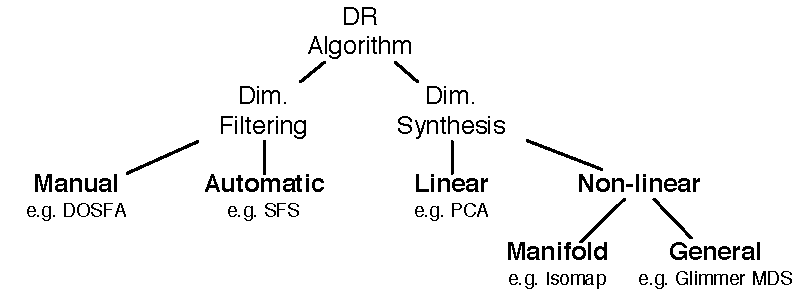
\includegraphics[width=\textwidth]{figures/dritw-dr-taxonomy}
    \caption
    [
        Our classification of dimensionality reduction algorithms.
    ]
    {
        Our classification of dimensionality reduction algorithms as either dimensional fitlering or dimensional synthesis. References: DOSFA (Dimension Ordering, Spacing and Filtering Approach)~\cite{Yang2003}, \ac{SFS}~\cite{Jain2000}, \ac{PCA}~\cite{Jolliffe2002}, Isomap~\cite{Tenenbaum2000}, Glimmer \ac{MDS}~\cite{Ingram2009}.
    }
    \label{fig:dritw-dr-taxonomy}
    \centering
\end{figure}

%-|-|-|-|-|-|-|-|-|-|-|-|-|-|-|-|-|-|-|-|-|-|-|-|-|-|-|-|-|-|-|-|-|-|-|-|-

This classification reflects distinctions that are well-known in the technical literature, but at a granularity suitable for the discussion of this manuscript that is simpler than many previous classification systems. 
It also emphasizes the types of algorithms\index{algorithms} used by the analysts we interviewed. 
Our choice of terms follows the vocabulary of the visualization community, rather than that of machine learning\index{machine learning} or other communities in which \ac{DR}\index{dimensionality reduction (DR)} is also used.

At a high level, \ac{DR}\index{dimensionality reduction (DR)} algorithms\index{algorithms} can be divided into {\it dimensional filtering}\index{dimensionality reduction (DR)!dimensional filtering}, in which less interesting dimensions are filtered out, and {\it dimensional synthesis}\index{dimensionality reduction (DR)!dimensional synthesis}, in which old dimensions are combined into new synthetic dimensions. 
In the machine learning\index{machine learning} literature, these categories are known as feature selection and feature extraction, respectively~\cite{Witten2011}. 

Dimensional filtering\index{dimensionality reduction (DR)!dimensional filtering} can be further differentiated between {\it manual} and {\it automatic} filtering techniques. 
Examples of manual filtering techniques are human-defined quality metrics for finding interesting dimensions~\cite{Johansson2009} and DOSFA (Dimensional Ordering, Spacing, and Filtering Approach)~\cite{Yang2003}. 
An example of an automatic filtering technique is \ac{SFS}\index{sequential forward selection (SFS)}~\cite{Jain2000} in which the ``best'' dimension is selected and others are added iteratively until no further improvement is made, relative to a threshold selected a priori.
In the visualization community, various techniques have been proposed that assist people in finding interesting two-dimensional projections of high-dimensional data\index{high-dimensional data}; in other words finding interesting two-dimensional scatterplots\index{visual encoding!scatterplot} in a \ac{SPLOM}\index{visual encoding!scatterplot!scatterplot matrix (SPLOM)}. 
Recent advances in this area, for instance, focus on finding two-dimensional projections that separate pre-defined clusters well~\cite{Sips2009,Tatu2010a}. 

Dimensional synthesis\index{dimensionality reduction (DR)!dimensional synthesis} is commonly differentiated between {\it linear} and {\it non-linear} techniques~\cite{Jain2000}. 
Linear techniques such as \ac{PCA}\index{dimensionality reduction (DR)!principal component analysis (PCA)}~\cite{Jolliffe2002}, Factor Analysis~\cite{Child2006}, or classical \ac{MDS}\index{dimensionality reduction (DR)!multi-dimensional scaling (MDS)} \cite{Torgerson1952,Young1938} produce new dimensions from linear projections of the original data.
Many datasets have an intrinsic structure that can only be revealed using non-linear techniques; these are further divided into {\it general} and {\it manifold} techniques. 
We define manifold techniques as the subset of non-linear techniques with the underlying assumption that the data lies on a densely sampled manifold.  
Of the numerous techniques that have been presented, some relevant examples include Isomap~\cite{Tenenbaum2000}, Laplacian Eigenmaps~\cite{Belkin2001}, Diffusion Maps~\cite{Coifman2005}, Maximum Variance Unfolding~\cite{Sha2005}, NeRV~\cite{Venna2007}, and Riemannian Manifold Learning~\cite{Lin2008}. 
Although the machine learning\index{machine learning} literature often uses the term manifold synonymously with non-linear, we distinguish manifold-specific techniques from general non-linear techniques. 
Examples of general techniques are the distance scaling MDS approach of Glimmer~\cite{Ingram2009}, and the multidimensional projection techniques Least Square Projection~\cite{Paulovich2008}, PLMP~\cite{Paulovich2010} and LAMP~\cite{Joia2011}. 
Some nonlinear dimensional synthesis\index{dimensionality reduction (DR)!dimensional synthesis} techniques straddle the two classes; for example, \citet{Chen2013} introduce a parametrized family of mapping techniques that can be tuned for either the general or manifold case.  
The operational distinction between manifold and general will become particularly important in \autoref{app:drvistasks:dritw:benchmarks}, where we discuss implications for benchmark datasets and relate them to manifold unrolling techniques. 

%-------------------------------------------------------------------------

\subsection{Methodology}
\label{app:drvistasks:dritw:methodology}

%-------------------------------------------------------------------------

We sought to better understand the tasks\index{task}, challenges, and context of high-dimensional data\index{high-dimensional data} analysts working in different domains.
To attain this understanding, we adopted a research methodology that alternated between cycles of data collection and analysis, allowing us to gradually identify and refine conceptual relationships grounded in the data~\cite{Charmaz2006}, as represented in \autoref{app:fig:dritw-methodology}. 
This methodological approach has been shown to be effective before, particularly in recent work on characterizing the processes undertaken by intelligence analysts~\cite{Kang2011} and enterprise data analysts~\cite{Kandel2012}, and the types of evaluation\index{evaluation} scenarios found in the visualization literature~\cite{Lam2012}. 

%-|-|-|-|-|-|-|-|-|-|-|-|-|-|-|-|-|-|-|-|-|-|-|-|-|-|-|-|-|-|-|-|-|-|-|-|-

\begin{figure}
    \centering
    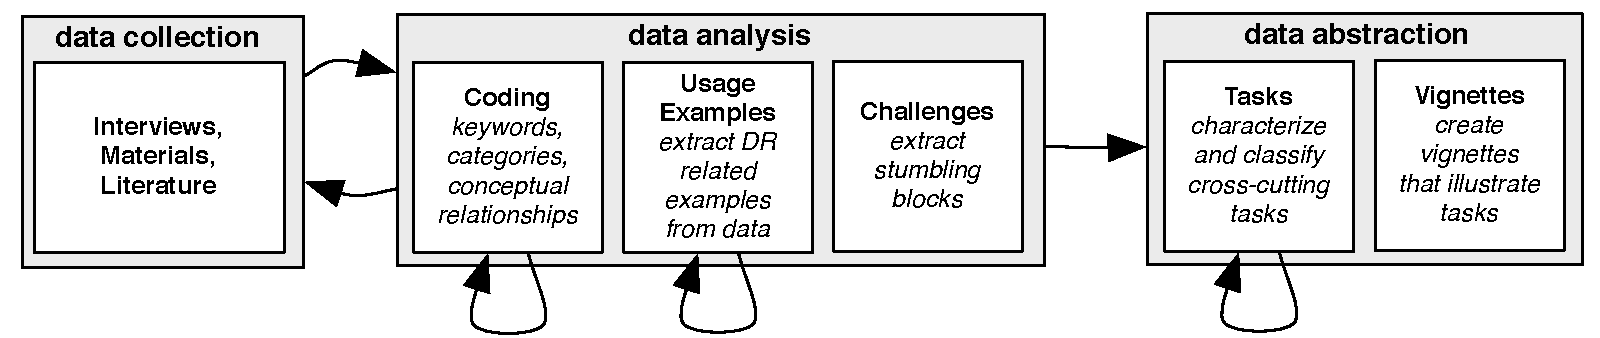
\includegraphics[width=\textwidth]{figures/dritw-methodology}
    \caption
    [
        Our data collection, analysis, and abstraction methodology.
    ]
    {
        Our data collection, analysis, and abstraction methodology. 
    }
    \label{app:fig:dritw-methodology}
    \centering
\end{figure}

%-|-|-|-|-|-|-|-|-|-|-|-|-|-|-|-|-|-|-|-|-|-|-|-|-|-|-|-|-|-|-|-|-|-|-|-|-

\bstart{``In the wild'' rationale}
We borrow the phrase ``in the wild''\index{evaluation!in the wild} from \ac{HCI}\index{human-computer interaction (HCI)}~\cite{Hollan2000}, where it differentiates investigation of people with their own work materials performing tasks\index{task} in real-world settings from studying human behavior in controlled laboratory settings; the goal of in-the-wild studies is maximizing the realism of findings \cite{McGrath1995}. 
The importance of better understanding the needs and visualization practices of people ``in the wild''\index{evaluation!in the wild} has been repeatedly raised in previous work by others~\cite{Carpendale2008,Isenberg2008,Plaisant2004} as well as in our own previous work~\cite{Munzner2009,Sedlmair2011}.

\bstart{Data collection}
We undertook several methods for studying the tasks\index{task} and challenges of high-dimensional data\index{high-dimensional data} analysts. 
Our primary method was semi-structured interviews. 

We interviewed nineteen high-dimensional data\index{high-dimensional data} analysts, recruited from our extended personal and professional networks\footnote{See summary in \autoref{tab:interviews}.}.
The analysts were sampled from a range of ten different domains, which included bioinformatics\index{bioinformatics}, machine learning\index{machine learning}, \ac{HCI}\index{human-computer interaction (HCI)}, policy analysis\index{policy analysis}, and journalism\index{journalism}. 
The majority of our analysts were academic researchers, ranging in years of experience from graduate students to senior professors. 
The remaining analysts were employed either by a national research lab, or by the private sector.

We conducted one or two interviews per data analyst, ranging in duration from thirty minutes to four hours. 
Most interviews were individual interviews while others were group interviews with multiple analysts working on similar problems. 
Whenever possible, we interviewed analysts at their place of work; others were conducted over the phone or using Skype. 

We used a set of open-ended questions relating to high-dimensional data\index{high-dimensional data} and \ac{DR}\index{dimensionality reduction (DR)}, which evolved over the course of data collection and analysis. 
We asked our interviewees about both projects from their past as well as ongoing work; in each interview, we sought to understand\footnote{See \autoref{app:drvistasks:interview-foci} for the complete interview question list.}: 

\begin{itemize}
    \item What are the goals, questions, or hypotheses that drive analysts?
    \item What data analysis tasks\index{task} do analysts undertake?
    \item Do these tasks\index{task} occur often? How long do they take? 
    \item What are the characteristics of analysts' datasets?
    \item How and when is \ac{DR}\index{dimensionality reduction (DR)} used? What role does visualization play?
    \item What are the major problems and challenges faced during the data analysis process?
    \item What are the patterns of interest? (clusters, outliers, correlation, semantically meaningful dimensions)
\end{itemize}

One to three interviewers guided the interview sessions.
We took extensive notes and audio recordings for later analysis, and we asked follow-up questions via email.

We also gathered materials from the analysts that we interviewed, which included their published papers, unpublished manuscripts, theses, datasets, and static images of their visualized data.

To broaden the corpus of data, we also surveyed the published \ac{DR}\index{dimensionality reduction (DR)} literature. 
To further enrich our data analysis, we chose to additionally include a small number of papers that featured the application of \ac{DR}\index{dimensionality reduction (DR)} for solving a particular domain problem; we excluded many papers that simply present a new \ac{DR}\index{dimensionality reduction (DR)} technique or algorithm\index{algorithms} without a detailed discussion of using it to solve a real-world problem. 

We concurrently performed data collection and analysis, culminating in the representation of our findings in the set of \ac{DR}\index{dimensionality reduction (DR)} tasks\index{task} described in \autoref{app:drvistasks:dritw:taxonomy}, as well as an understanding of the challenges faced by high-dimensional data\index{high-dimensional data} analysts, discussed in \autoref{app:drvistasks:dritw:challenges}.
The analysis process yielded five types of results.

\bstart{Coding} 
Interview notes and other materials collected were iteratively coded to identify conceptual relationships into higher-level categories \cite{Charmaz2006}. 
These codes spanned analysts' high-level research goals\index{task!high-level tasks}, their expertise and assumptions, the structure and size of their dataset(s), their current analysis techniques and approaches, the challenges they faced, as well as desired or actual outcomes. 
This code set provided us with an intermediate result that we used for further analysis.

\bstart{Usage examples} 
Using our refined set of codes, we iteratively constructed and revised twenty-seven concise and distinct \ac{DR}\index{dimensionality reduction (DR)} {\it usage examples}: twenty-two from interviews and five from our literature review; these are summarized in \autoref{table:dritw-table-2}.
A usage example includes a description of an analyst's task\index{task} as well as the means\index{task!means} by which they perform this task\index{task}.

While most of the interviews resulted in one usage example, several analysts described multiple yet fundamentally different analysis situations in which they used or wanted to use \ac{DR}\index{dimensionality reduction (DR)}; these became multiple usage examples, allowing for a concise description using our set of abstract tasks\index{task!task abstraction}. 
In the case of one interviewee, we did not have enough information to derive a concise usage example, so this data was excluded from subsequent analysis.
Additionally, we derived five usage examples from the literature with interesting descriptions of high-dimensional data\index{high-dimensional data} analysis and \ac{DR}\index{dimensionality reduction (DR)} \cite{Bronstein2006,Buja2002,Matusik2003,Reveret2005,Tenenbaum2000}. 
These examples were unusual in that they contained sufficient detail about the data analysis process itself to support a usage example; we considered dozens of other technical papers that did not, but instead focused exclusively on algorithmic issues\index{algorithms}. 

\bstart{Challenges} 
Our analysts also described problems they faced while performing \ac{DR}\index{dimensionality reduction (DR)} tasks\index{task}. 
We report these challenges in \autoref{app:drvistasks:dritw:challenges}, relate them to the technical literature, and discuss implications for the design of high-dimensional data\index{high-dimensional data} analysis tools and techniques. 

\bstart{Tasks} 
We then broke down the usage examples into smaller units of concrete and abstract tasks\index{task!task abstraction}. 
We iteratively explored different levels of task abstractions\index{task!task abstraction} and organization, and evaluated\index{evaluation} them across the usage examples.  
The final results are the hierarchical organization shown in \autoref{fig:dritw-taxonomy-2}.

\bstart{Vignettes}
Finally, we created descriptive {\it vignettes} based on our usage examples and task\index{task} classification, 
to ground our written discussion of these tasks\index{task} in our collected data. 
These vignettes, featured in \autoref{app:drvistasks:dritw:taxonomy}, provide concise and highly abstract summaries of an analyst's task\index{task!task abstraction}. 
In contrast, unprocessed direct quotes from interviews would be prohibitively lengthy and moreover would be framed in the vocabulary of the particular domain, impeding cross-domain abstraction\index{task!task abstraction}. 
The importance of such abstractions\index{task!task abstraction} and its challenges have been discussed in our previous work~\cite{Munzner2009,Sedlmair2012}.

Further details about our methodological approach can be found in the supplemental material.

%-------------------------------------------------------------------------

\subsection{Taxonomy}
\label{app:drvistasks:dritw:taxonomy}

%-------------------------------------------------------------------------

\autoref{fig:dritw-taxonomy-2} presents our findings in terms of tasks\index{task} involving \ac{DR}\index{dimensionality reduction (DR)} usage for high-dimensional data\index{high-dimensional data} analysis. 
Rectangular nodes represent tasks\index{task} and oval nodes represent interests that further characterize tasks\index{task}.

%-|-|-|-|-|-|-|-|-|-|-|-|-|-|-|-|-|-|-|-|-|-|-|-|-|-|-|-|-|-|-|-|-|-|-|-|-

\begin{figure}
    \centering
    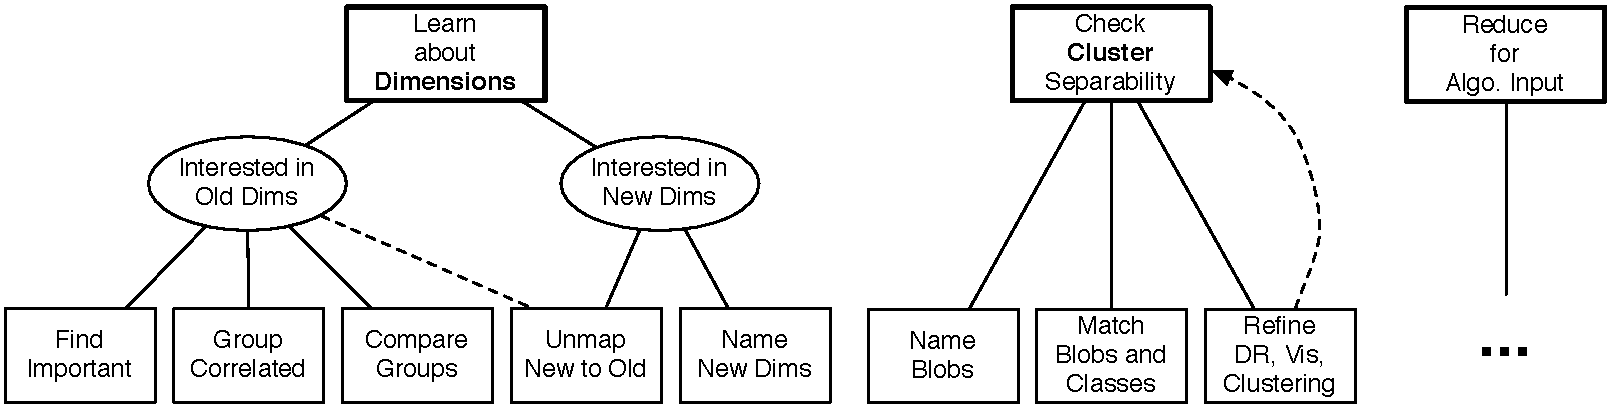
\includegraphics[width=\textwidth]{figures/dritw-taxonomy-2}
    \caption
    [
        Our classification of tasks relating to \ac{DR}.
    ]
    {
        Our classification of tasks relating to \ac{DR}.
    }
    \label{fig:dritw-taxonomy-2}
    \centering
\end{figure}

%-|-|-|-|-|-|-|-|-|-|-|-|-|-|-|-|-|-|-|-|-|-|-|-|-|-|-|-|-|-|-|-|-|-|-|-|-

%-|-|-|-|-|-|-|-|-|-|-|-|-|-|-|-|-|-|-|-|-|-|-|-|-|-|-|-|-|-|-|-|-|-|-|-|-

\begin{table}
    \centering
    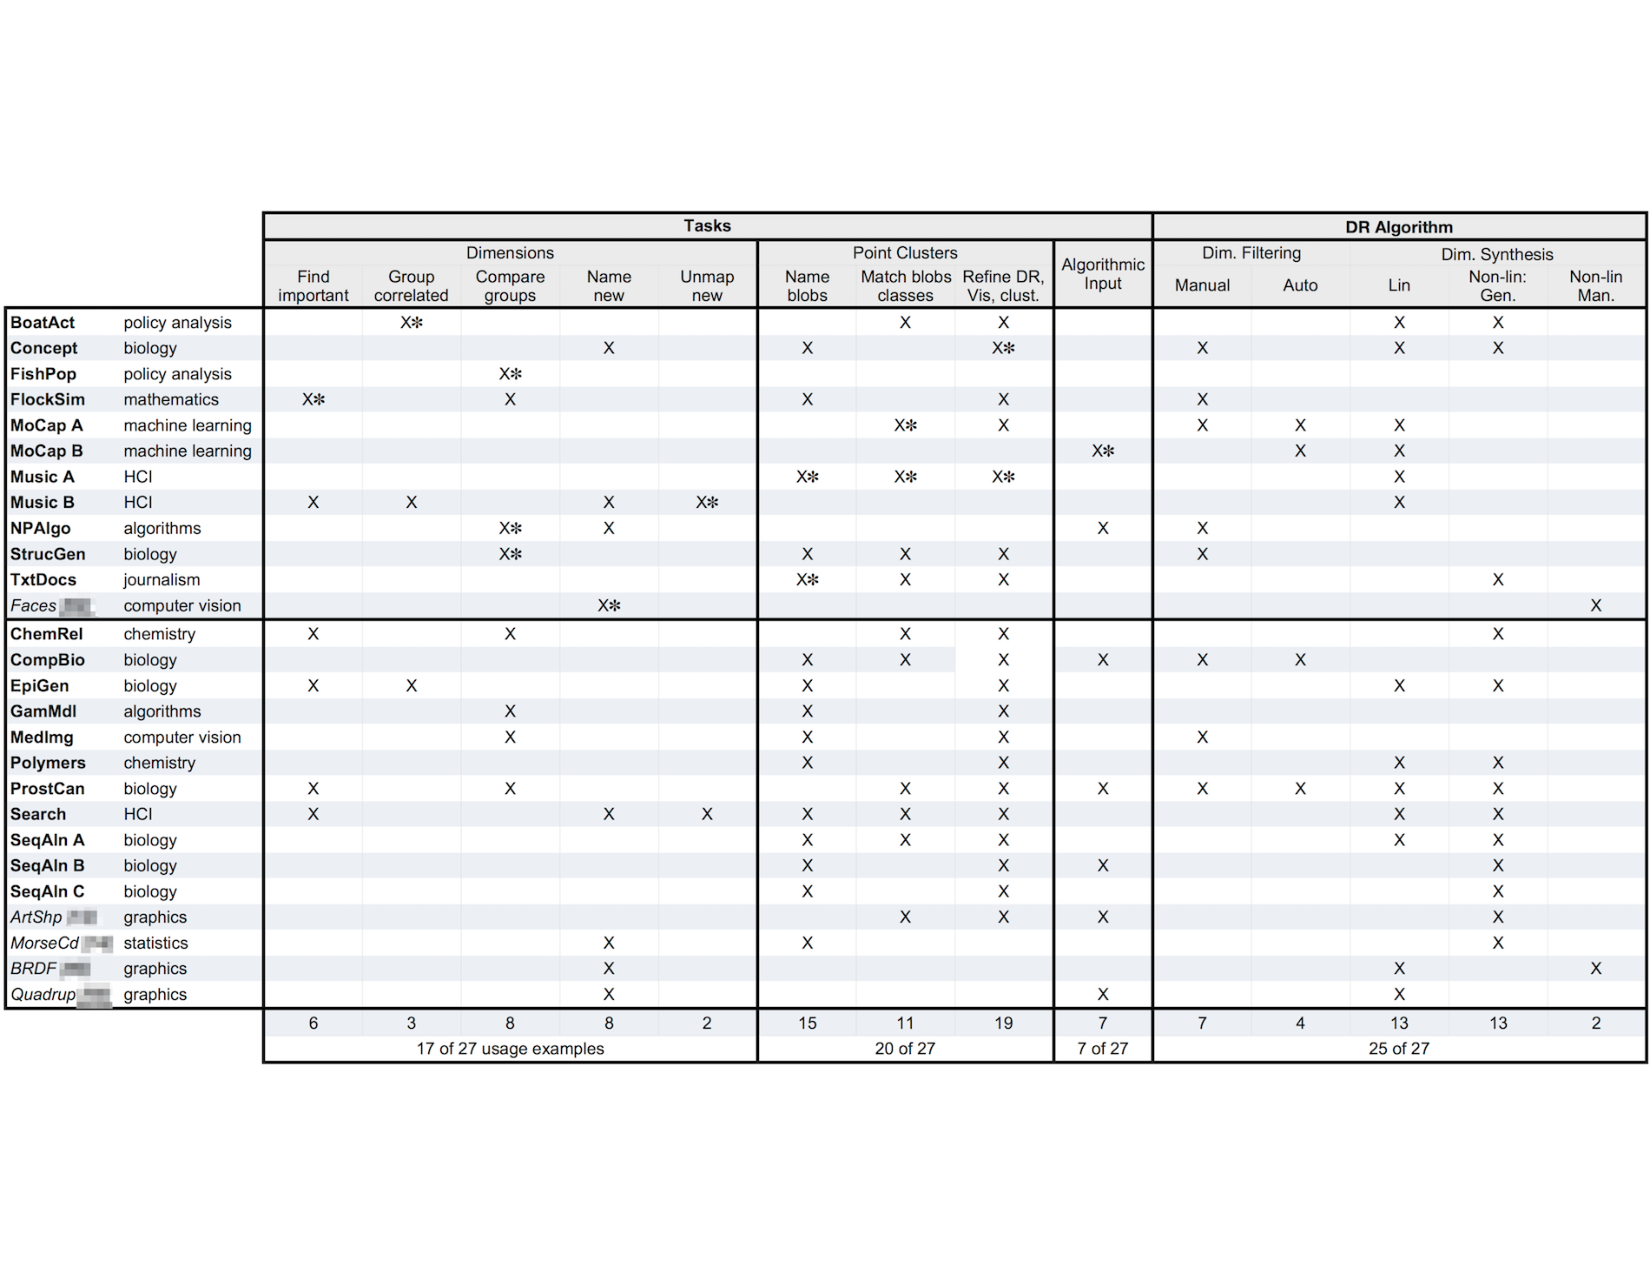
\includegraphics[width=\textwidth]{figures/dritw-table-2.pdf}
    \caption
    [
        Usage examples described using our classification of tasks relating to \ac{DR}. 
    ]
    {
        Usage examples described using our classification of tasks relating to \ac{DR}. Asterisks indicate tasks that we describe in vignettes. Paper references: {\sc Faces}~\cite{Tenenbaum2000}, {\sc ArtShp}~\cite{Bronstein2006}, {\sc MorseCd}~\cite{Buja2002}, {\sc BRDF}~\cite{Matusik2003}, {\sc Quadrup}~\cite{Reveret2005}. The usage examples abbreviations correspond to analyst ID numbers listed in \autoref{tab:interviews}. 
    }
    \label{table:dritw-table-2}
    \centering
\end{table}

%-|-|-|-|-|-|-|-|-|-|-|-|-|-|-|-|-|-|-|-|-|-|-|-|-|-|-|-|-|-|-|-|-|-|-|-|-

At the top level, we distinguish between three different intents of using \ac{DR}\index{dimensionality reduction (DR)}: using \ac{DR}\index{dimensionality reduction (DR)} to learn about {\it dimensions}, both the given {\it old} dimensions as well as synthesized {\it new} dimensions, using \ac{DR}\index{dimensionality reduction (DR)} to see {\it point clusters}, and finally using \ac{DR}\index{dimensionality reduction (DR)} for reducing data for {\it algorithmic input}\index{algorithms!algorithmic input}. 

Our analysis focuses predominantly on the former two, dimensions and point clusters, which involve \ac{DR}\index{dimensionality reduction (DR)} usage as part of the data analysis process. 
Both of these high-level tasks\index{task!high-level tasks} are hierarchically broken further down into mid-level tasks\index{task!mid-level tasks}.
We specifically abstained from breaking them down into all of their lowest-level components, since low-level interactive visualization tasks\index{task!low-level tasks} are adequately classified in previous work~\cite{Amar2005,Shneiderman1996,Yi2007}.
Instead, we focus on revealing meaningful mid-level tasks\index{task!mid-level tasks}. 

For tasks\index{task} relating to dimensions and point clusters, analysts often used \ac{DR}\index{dimensionality reduction (DR)} with the intent of visualizing the dimensionally reduced data\index{dimensionality reduction (DR)}, using visual encodings\index{visual encoding} such as two-dimensional scatterplots\index{visual encoding!scatterplot} (twenty usage examples), three-dimensional scatterplots\index{visual encoding!scatterplot!3D scatterplot} (three usage examples) or a \ac{SPLOM}\index{visual encoding!scatterplot!scatterplot matrix (SPLOM)} (two usage examples). 
Nevertheless, we also found instances where analysts were using \ac{DR}\index{dimensionality reduction (DR)} for the purpose of data analysis without subsequently visualizing the low-dimensional data, such as the {\sc Music B} (\ref{drvistasks:analyst:JB}) usage example discussed below. 

As a third high-level task\index{task!high-level tasks}, we include using \ac{DR}\index{dimensionality reduction (DR)} for algorithmic input\index{algorithms!algorithmic input}. 
Here, \ac{DR}\index{dimensionality reduction (DR)} is used as a means\index{task!means} of automatic data compression and noise reduction rather than for explorative data analysis. 
We provide this task\index{task} as important context, however we do not go into depth as with the other two task\index{task} categories. 
The power of using \ac{DR}\index{dimensionality reduction (DR)} for the purpose of algorithmic input\index{algorithms!algorithmic input} has been widely discussed in the machine learning\index{machine learning} and data mining communities~\cite{Bingham2001,Murphy2012}\index{data mining}. 

%-------------------------------------------------------------------------

\subsubsection{DR for Learning About Dimensions}
\label{app:drvistasks:dritw:taxonomy:dimensions}

%-------------------------------------------------------------------------

We found seventeen usage examples in which analysts were interested in learning about the dimensions of a dataset, reflected in the left-most branch of \autoref{fig:dritw-taxonomy-2}.
We differentiate between interests in the original high-dimensional, or {\it old}, dimensions, and interests in the {\it new} dimensions that are the result of dimensional synthesis\index{dimensionality reduction (DR)!dimensional synthesis} \ac{DR}\index{dimensionality reduction (DR)} algorithms. 
Since a single data analyst can be engaged in multiple tasks\index{task}, having interests in both old and new dimensions within the same usage example is not uncommon. 

\bstart{Find important old dimensions} 
We identified six usage examples in which the analyst sought to {\it find important old} dimensions in a dataset, according to some particular metric of interest, for example the variance that a single dimension contributes to the overall variance.

\begin{quotation}
    In the {\sc FlockSim} usage example, a mathematician (\ref{drvistasks:analyst:ASN}) was interested in modeling self-organized aggregate animal behavior; in the case of birds, this is known as flock behavior. 
    Her dataset of recorded flock behavior contained fourteen spatiotemporal dimensions.
    A desirable model would accurately and precisely predict flock behavior, such as where a flock may land. 
    The model would also need to strike a balance between sensitivity\index{sensitivity analysis} and computation time; a model with two to three spatiotemporal dimensions was therefore thought to be ideal.
    Additionally, the model parameters should retain the semantics of the original dimensions. 
    Thus the analyst's task\index{task} is one of {\it finding the most important dimensions} in the recorded flock data, examining which dimensions contribute heavily to the overall variance. 
    She did that by manually filtering and inspecting all fourteen dimensions. 
\end{quotation}

For identifying important dimensions, analysts usually engage in manual or automatic filtering of dimensions. Some also used linear dimensional synthesis\index{dimensionality reduction (DR)!dimensional synthesis} techniques such as \ac{PCA}\index{dimensionality reduction (DR)!principal component analysis (PCA)}, as in the {\sc Music B} (\ref{drvistasks:analyst:JB}) example discussed below.

\bstart{Group correlated old dimensions} 
Analysts may also be interested in grouping old dimensions. 
Usually, this grouping is done by consolidating singleton dimensions that are correlated together into groups.
We identified three usage examples where the analyst engaged in {\it grouping correlated} dimensions. 
In these cases linear \ac{DR}\index{dimensionality reduction (DR)} techniques were used as indicators for dimensional correlation.

\begin{quotation}
    \begin{sloppypar}
    In the {\sc BoatAct} usage example, a geographic information systems (GIS) analyst (\ref{drvistasks:analyst:CM}) was interested in characterizing travel patterns of recreational boaters, which carry implications for maritime traffic routing.
    Using a questionnaire with thirty-nine items, she surveyed five hundred and forty-three recreational boaters about their boating practices and preferences. 
    The analyst wanted to better understand the correlation among the thirty-nine dimensions of her survey and to group correlated dimensions together. To learn about the correlation of dimensions, she used \ac{PCA}\index{dimensionality reduction (DR)!principal component analysis (PCA)} to provide her with a rough understanding of which dimensions she might group together.
    After manually assigning dimensions to groups, she aggregated the groups. 
    Then she used both the aggregation and the dimensions of a group to describe different recreational boating patterns.
    \end{sloppypar}
\end{quotation}

\bstart{Compare groups of old dimensions} 
In eight usage examples, datasets were comprised of groups of dimensions. 
These groups might be known a priori, or might be manually created by an analyst during the analysis process, such as by grouping correlated dimensions as described above. 
The most typical case is when a dataset was produced by a predictive simulation model, where there exists a group of independent, or {\it input} dimensions and a group of dependent, or {\it output} dimensions\footnote{Different communities use different vocabularies for these types of dimensions with independent/dependent, cause/effect, and input/output being the most common ones. 
We opted for input/output because it was frequently used by our interviewees and is common for describing simulation models.}.
When groups of dimensions exist, one common task\index{task} is to {\it compare these dimensional groups}, which might or might not coexist with a need for \ac{DR}\index{dimensionality reduction (DR)}. 

\begin{quotation}
    In the {\sc NPAlgo} usage example, a computer scientist (\ref{drvistasks:analyst:KLB}) was interested in using empirical methods to construct good prediction models for algorithms\index{algorithms} solving NP-hard problems, such as the traveling salesman problem.
    He measured the time required to run an algorithm\index{algorithms} for a NP-hard problem across many different parameter settings, where the settings are regularly sampled from the available range. 

    This process results in a dataset with between one hundred thousand and one million points, with two groups of dimensions: a group of approximately one hundred input dimensions representing parameter choices, and the measured runtime as a single output dimension. 
    The dataset is then used to train a predictive model for the algorithm\index{algorithms} at hand. 
    Although the resulting prediction model works well, humans have a hard time understanding this one-hundred-dimensional feature space. 
    The analyst sought a way to reduce the dataset to a lower dimensional set of five-ten input dimensions, with a resulting model that retains nearly the same predictive power as the one that uses the entire feature space. 
    The data analyst knew that the input dimensions are highly correlated to each other, so he wanted to use a dimensional synthesis\index{dimensionality reduction (DR)!dimensional synthesis} technique.
\end{quotation}

Abstractly, the goal of this analyst can be described as getting insight\index{insight} into {\it groups of dimensions} and to synthesize {\it new dimensions} without diminishing predictive power.
In \autoref{app:drvistasks:dritw:challenges}, we will further discuss this usage example and see that this combination is not well supported by current state-of-the-art \ac{DR}\index{dimensionality reduction (DR)} algorithms\index{algorithms}.

In five of the eight usage examples involving groups of dimensions, there existed two groups of dimensions, having an input/output relationship.  
The remaining three usage examples involved the more general case of $n$ groups of dimensions.  

\begin{quotation}
    \begin{sloppypar}
    The {\sc StrucGen} usage example involved a bioinformatician\index{bioinformatics} (\ref{drvistasks:analyst:JWB}) with three explicit groups of dimensions in his protein dataset: one group pertaining to proteins' three-dimensional structure as described by high-dimensional feature vectors, one describing proteins within a hierarchical organization of functional properties, and another pertaining to the ordering of amino acid sequences within these proteins. 
    His task\index{task} was to identify similarities and differences across these groups of dimensions. 
    He independently reduced the dimension of all three groups by manually filtering them, and then sought to understand the relationships between them.
    \end{sloppypar}
\end{quotation}

In general, comparing groups of dimensions can stem from different interests of an analyst. 
A typical interest is to learn about how groups correlate to each other. 
Another example is sensitivity analysis\index{sensitivity analysis}, where the goal is to understand whether small changes within one set of dimensions lead to small or large changes in another set of dimensions~\cite{Booshehrian2012,Piringer2010,Pretorius2011}. 
Sensitivity analysis\index{sensitivity analysis} is particularly common with predictive simulation models, to understand the sensitivity of output dimensions to changes on input dimensions. 
A recent example of use cases in which sensitivity analysis\index{sensitivity analysis} is combined with \ac{DR}\index{dimensionality reduction (DR)} can be found in \citet{Bergner2013}.
While these tasks\index{task} can co-exist with \ac{DR}\index{dimensionality reduction (DR)}, they can also occur without any need of \ac{DR}\index{dimensionality reduction (DR)}. In \autoref{app:drvistasks:dritw:challenges}, we will discuss one such usage example.

\bstart{Name new dimensions} 
Tasks\index{task} involving an interest in new dimensions necessarily imply the usage of dimension synthesis techniques. 
One common task\index{task} is to {\it name new} dimensions, which we found in eight usage examples. Here, the analyst attempts to ascertain the semantic meaning of the proposed new dimensions. 
A common approach is to inspect the original high-dimensional data\index{high-dimensional data} plotted within the context of the new low-dimensional layout in a scatterplot\index{visual encoding!scatterplot}, wherein the analyst may be able to discern an interesting semantic relationship along the low-dimensional axes: the task\index{task} of {\it naming new} dimensions is often used in \ac{DR}\index{dimensionality reduction (DR)} algorithm\index{algorithms} papers~\cite{Buja2002,Tenenbaum2000}, in particular those about non-linear \ac{DR}\index{dimensionality reduction (DR)} techniques:

\begin{quotation}
    In the {\sc Faces} usage example~\cite{Tenenbaum2000}, a dataset of human face images, with each image described by a vector with four thousand and ninety-six, was reduced to three dimensions to showcase the capabilities of the Isomap algorithm\index{algorithms}. 
    In the low-dimensional space, it became possible to plot the images as thumbnails in a scatterplot\index{visual encoding!scatterplot}, whereupon three meaningful dimensions were identified: up-down pose, left-right pose, and illumination. 
\end{quotation}

While many of the {\it naming new dimensions} examples are from the literature (four usage examples), we also detected these tasks\index{task} in our field investigation (four usage examples). 

\bstart{Unmap new dimensions to old dimensions} 
Another task\index{task} associated with new dimensions is {\it unmapping} new dimensions to corresponding old dimensions. 
Unmapping can be conducted in a straightforward fashion with linear techniques, by inspecting the extent to which any particular old dimension contributed to the synthesis of a new one. 
In PCA, unmapped old dimensions are often referred to as the ``loading'' of the (new) dimensions \cite{Jolliffe2002}.

\begin{quotation}
    The {\sc Music} analyst (\ref{drvistasks:analyst:JB}) was interested in the listening behavior of digital music consumers. 
    She gathered listening history data and demographic information from approximately three hundred people who use the last.fm music streaming service\footnote{\url{http://last.fm/}.}. 
    The resulting dataset had forty-eight dimensions, which included continuous dimensions, such as the number of tracks streamed per day or per login session, as well as categorical dimensions, which included the gender and geographical location of a person using last.fm.
    
    In the {\sc Music B} usage example, she engaged in finding important dimensions and consolidating dimensions by correlating them into groups. With a set of grouped dimensions she intended to characterize and describe important factors in music listening behavior. 
    She used \ac{PCA}\index{dimensionality reduction (DR)!principal component analysis (PCA)} and examined the first thirteen principal components, which accounted for seventy-five percent of the variance. 
    Her goal was to account for as much of the variance of the original data as possible with a small number of new dimensions, while maintaining an understandable semantic mapping between old and new dimensions. 
    By closely analyzing this unmapping, she identified proper names and meanings for the new synthetic thirteen dimensions.
    She did not visualize her data in this analysis.
\end{quotation}

With linear \ac{DR}\index{dimensionality reduction (DR)} techniques, such as \ac{PCA}\index{dimensionality reduction (DR)!principal component analysis (PCA)}, the relation between old and new dimensions is clear.
However, most non-linear techniques, while offering a more powerful reduction, do not support unmapping: the mapping that occurs between old and new dimensions is hard to interpret. 

The unmapping approach is a top-down approach, in which first a \ac{DR}\index{dimensionality reduction (DR)} synthesis algorithm\index{algorithms} is used and then the loadings of the new dimensions are inspected. 
In contrast, a bottom-up approach can lead to similar results. 
Consider, for instance, the {\sc BoatAct} usage example, in which \ref{drvistasks:analyst:CM} first learned about the correlation of the old dimensions, grouped them together accordingly, and then aggregated them into new synthetic ones. 
Both approaches can lead to similar outcomes. 

\bstart{No correlation among new dimensions}
While we found that determining correlation between old dimensions is an important task\index{task}, we do not include correlation between new dimensions as a task\index{task}. 
We did not find any instances of analysts with this interest. 
We are not surprised by this finding, because many \ac{DR}\index{dimensionality reduction (DR)} techniques produce new synthetic dimensions that have as little correlation between them as possible; the best-known example is \ac{PCA}\index{dimensionality reduction (DR)!principal component analysis (PCA)}.
In these cases, searching for correlation between new synthetic dimensions is unlikely to yield meaningful results. 
Nevertheless, we call out this issue, in particular because we have seen arguments in the visualization literature that confound what we consider to be two very different uses of scatterplots\index{visual encoding!scatterplot}. 
The use of scatterplots\index{visual encoding!scatterplot} to show correlation in data that is not dimensionally reduced should not be conflated with the use of scatterplots\index{visual encoding!scatterplot} for dimensionally reduced data\index{dimensionality reduction (DR)} to name new dimensions or check for cluster separability. 

%-------------------------------------------------------------------------

\subsubsection{DR for Checking Cluster Separability}
\label{app:drvistasks:dritw:taxonomy:clusters}

%-------------------------------------------------------------------------

\ac{DR}\index{dimensionality reduction (DR)}-related clustering tasks\index{task} pertain to the identification and verification of separable point clusters in the data (twenty usage examples), reflected in the middle branch of \autoref{fig:dritw-taxonomy-2}. 
In terms of visual data analysis, clustering is strongly tied to visualizing dimensionally reduced data\index{dimensionality reduction (DR)} in scatterplots\index{visual encoding!scatterplot}: eighteen of the twenty usage examples associated with an interest in clusters involved the use of scatterplots\index{visual encoding!scatterplot}.

If there is no {\it class structure} available, these scatterplots\index{visual encoding!scatterplot} are typically shown in monochrome and a common task\index{task} is to identify and {\it name separable blobs}, and to see if these blobs match the analyst's mental model of the dataset. 
By separable blobs, we refer to proximity relationships in the lower-dimensional layout of points, forming a distinguishable structure as shown in \autoref{app:drvistasks:fig:clusters}a.  

On the other hand, a dataset often comes with an associated class structure, which is then typically shown by color coding points according to their classes. 
These classes might come directly with the data, be assigned using a clustering algorithm\index{algorithms!clustering} run by the analyst, or be the result of manual labeling.   
Here, we found that the predominant reason that people look at scatterplots\index{visual encoding!scatterplot} is to check if separable blobs match with the color-coded classes as shown in \autoref{app:drvistasks:fig:clusters}b and \autoref{app:drvistasks:fig:clusters}c. 
Note that we previously found~\cite{Sedlmair2012a} that the visual separability of color-coded clusters differs perceptually from the separability of monochrome clusters.

The more common situation however is that the visualization of dimensionally reduced data\index{dimensionality reduction (DR)} does not lead to clearly separable blobs. Rather than clearly visible structure, reducing the dimension of the data and plotting it in a scatterplot\index{visual encoding!scatterplot} often leads to an undifferentiated clutter of points, as shown in \autoref{app:drvistasks:fig:clusters}d and \autoref{app:drvistasks:fig:clusters}e. 
In such situations, analysts often engage in iterative {\it refining of \ac{DR}\index{dimensionality reduction (DR)}, visual encoding\index{visual encoding}, and/or clustering} algorithms\index{algorithms!clustering} to obviate algorithmic\index{algorithms} artifacts as a reason for the non-visibility of cluster structure. 

%-|-|-|-|-|-|-|-|-|-|-|-|-|-|-|-|-|-|-|-|-|-|-|-|-|-|-|-|-|-|-|-|-|-|-|-|-

\begin{figure}
	\centering
	\begin{subfigure}[t]{0.45\textwidth}
	    \centering
        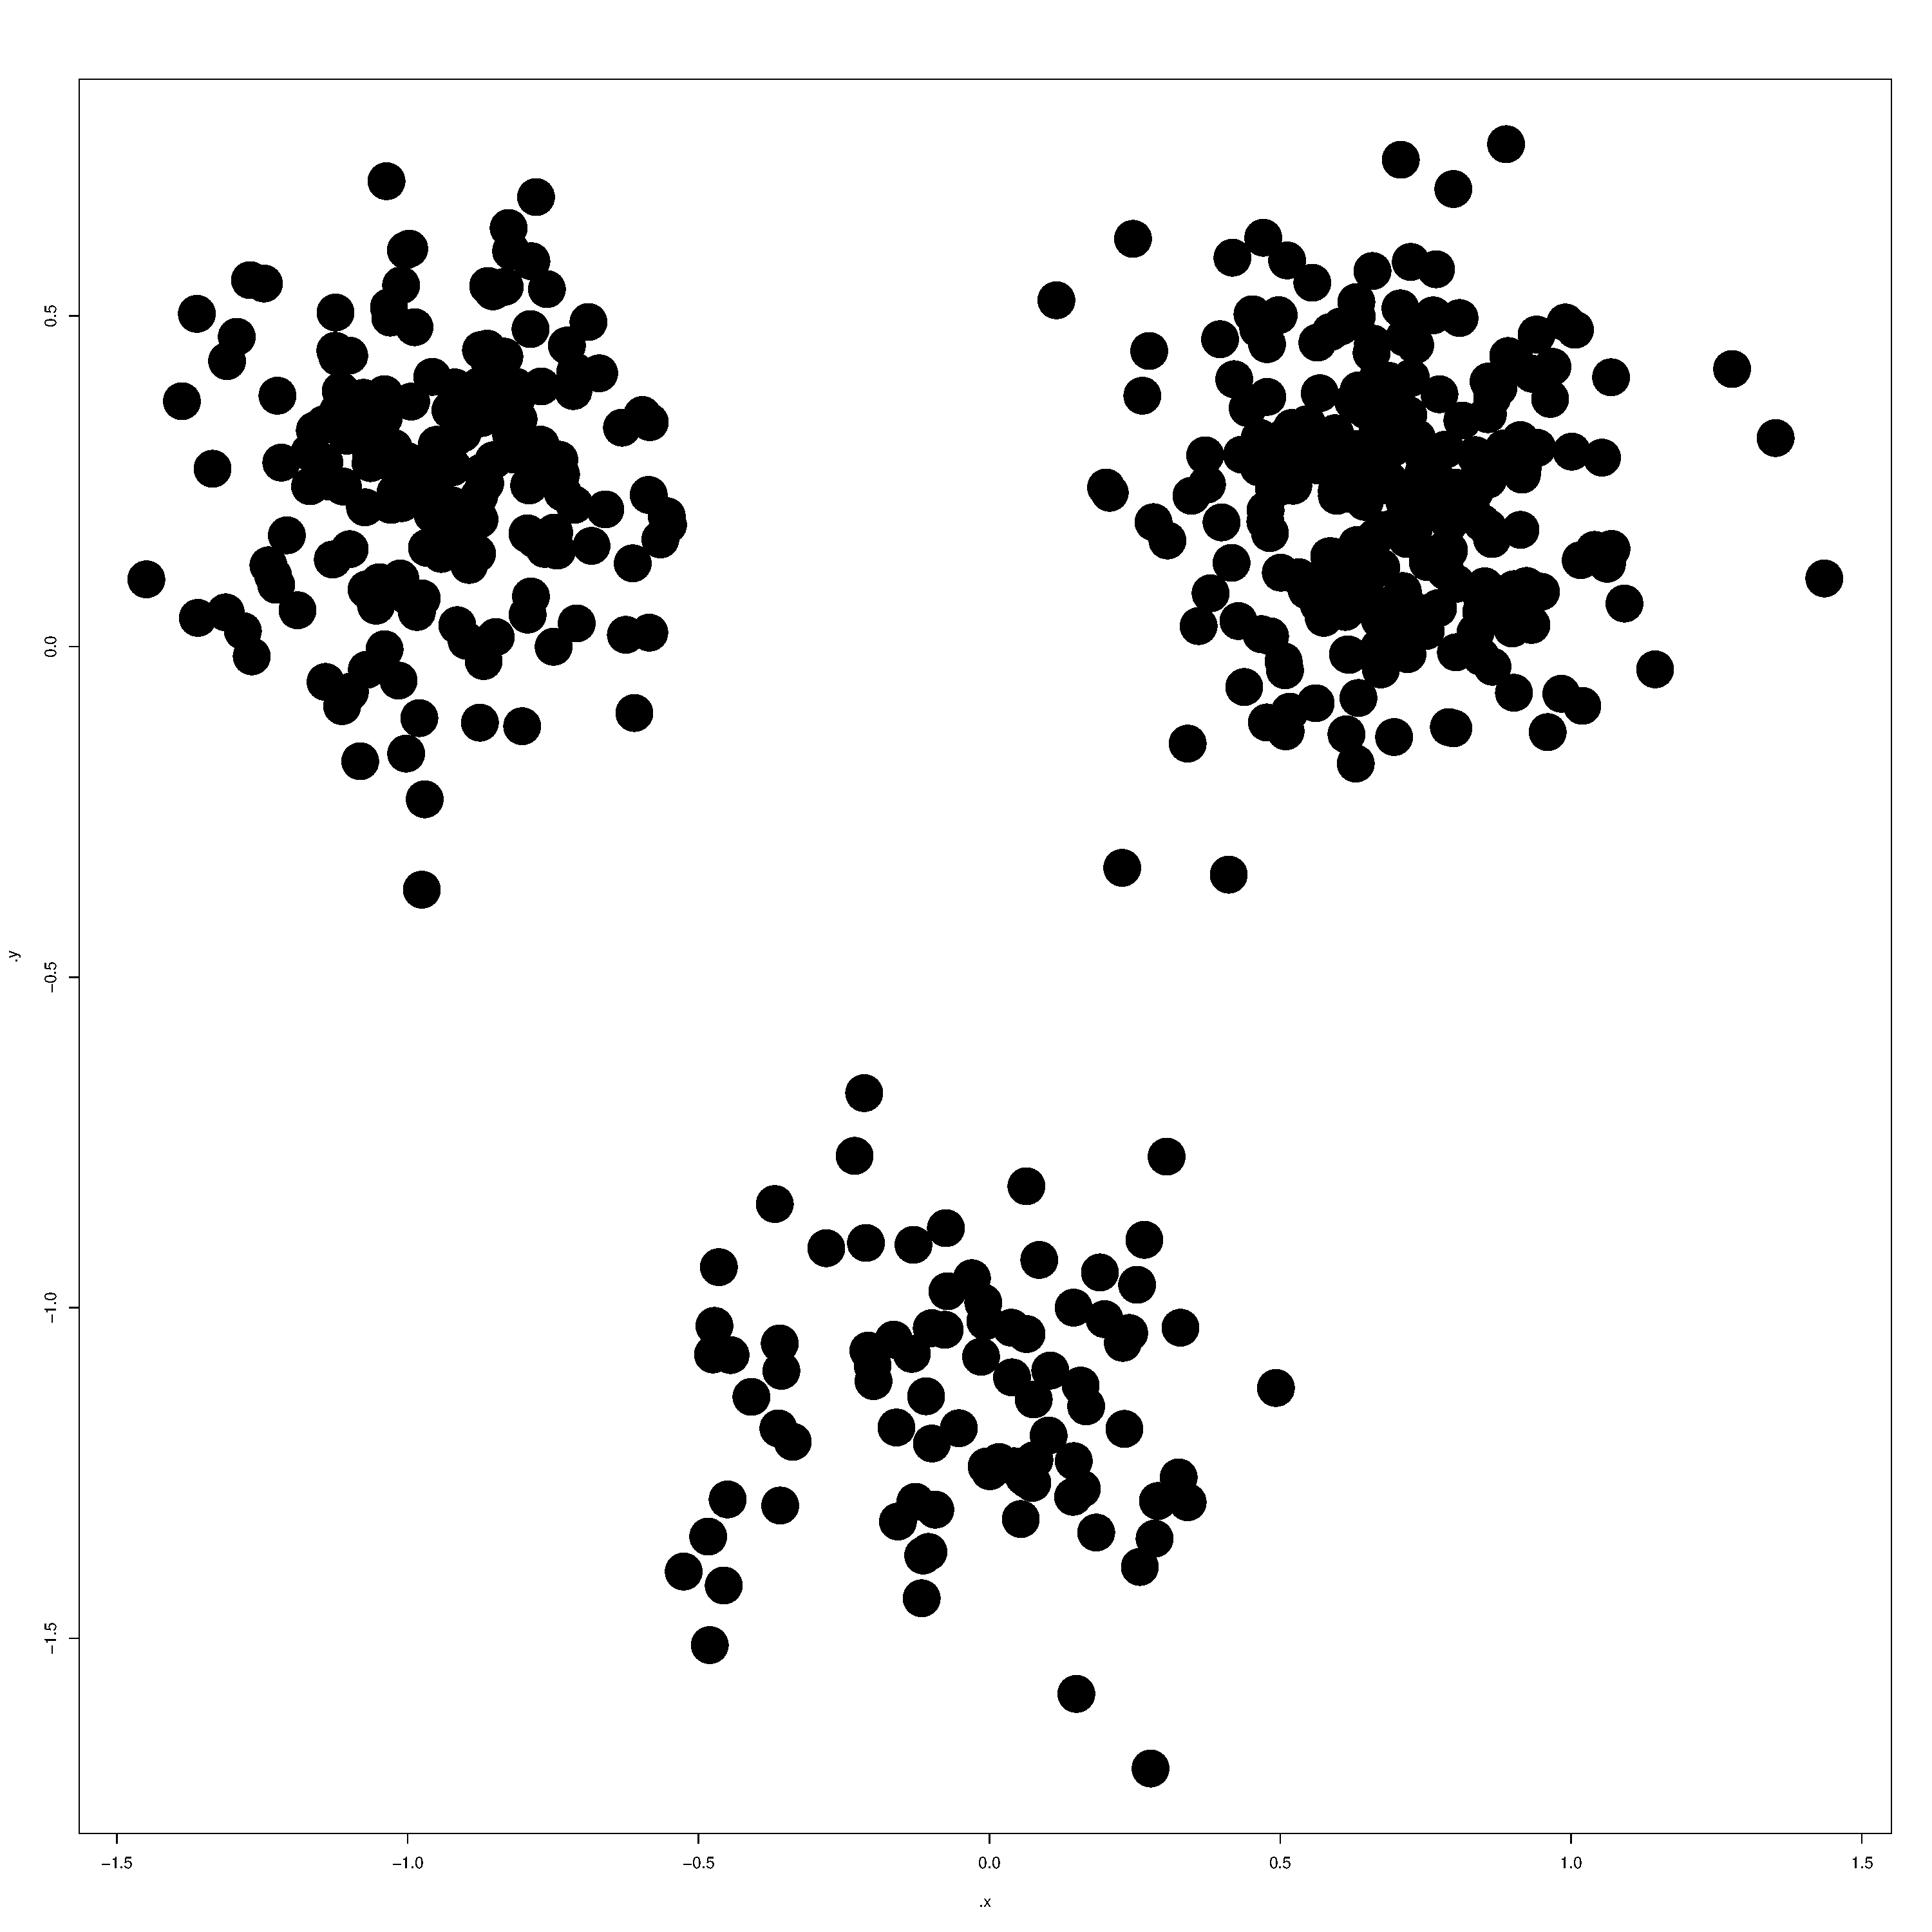
\includegraphics[height=2.5cm]{figures/clusters_impl.pdf}
        \caption{Naming separable blobs of unlabeled data.}
    \end{subfigure}
    ~
    \begin{subfigure}[t]{0.45\textwidth}
	    \centering
        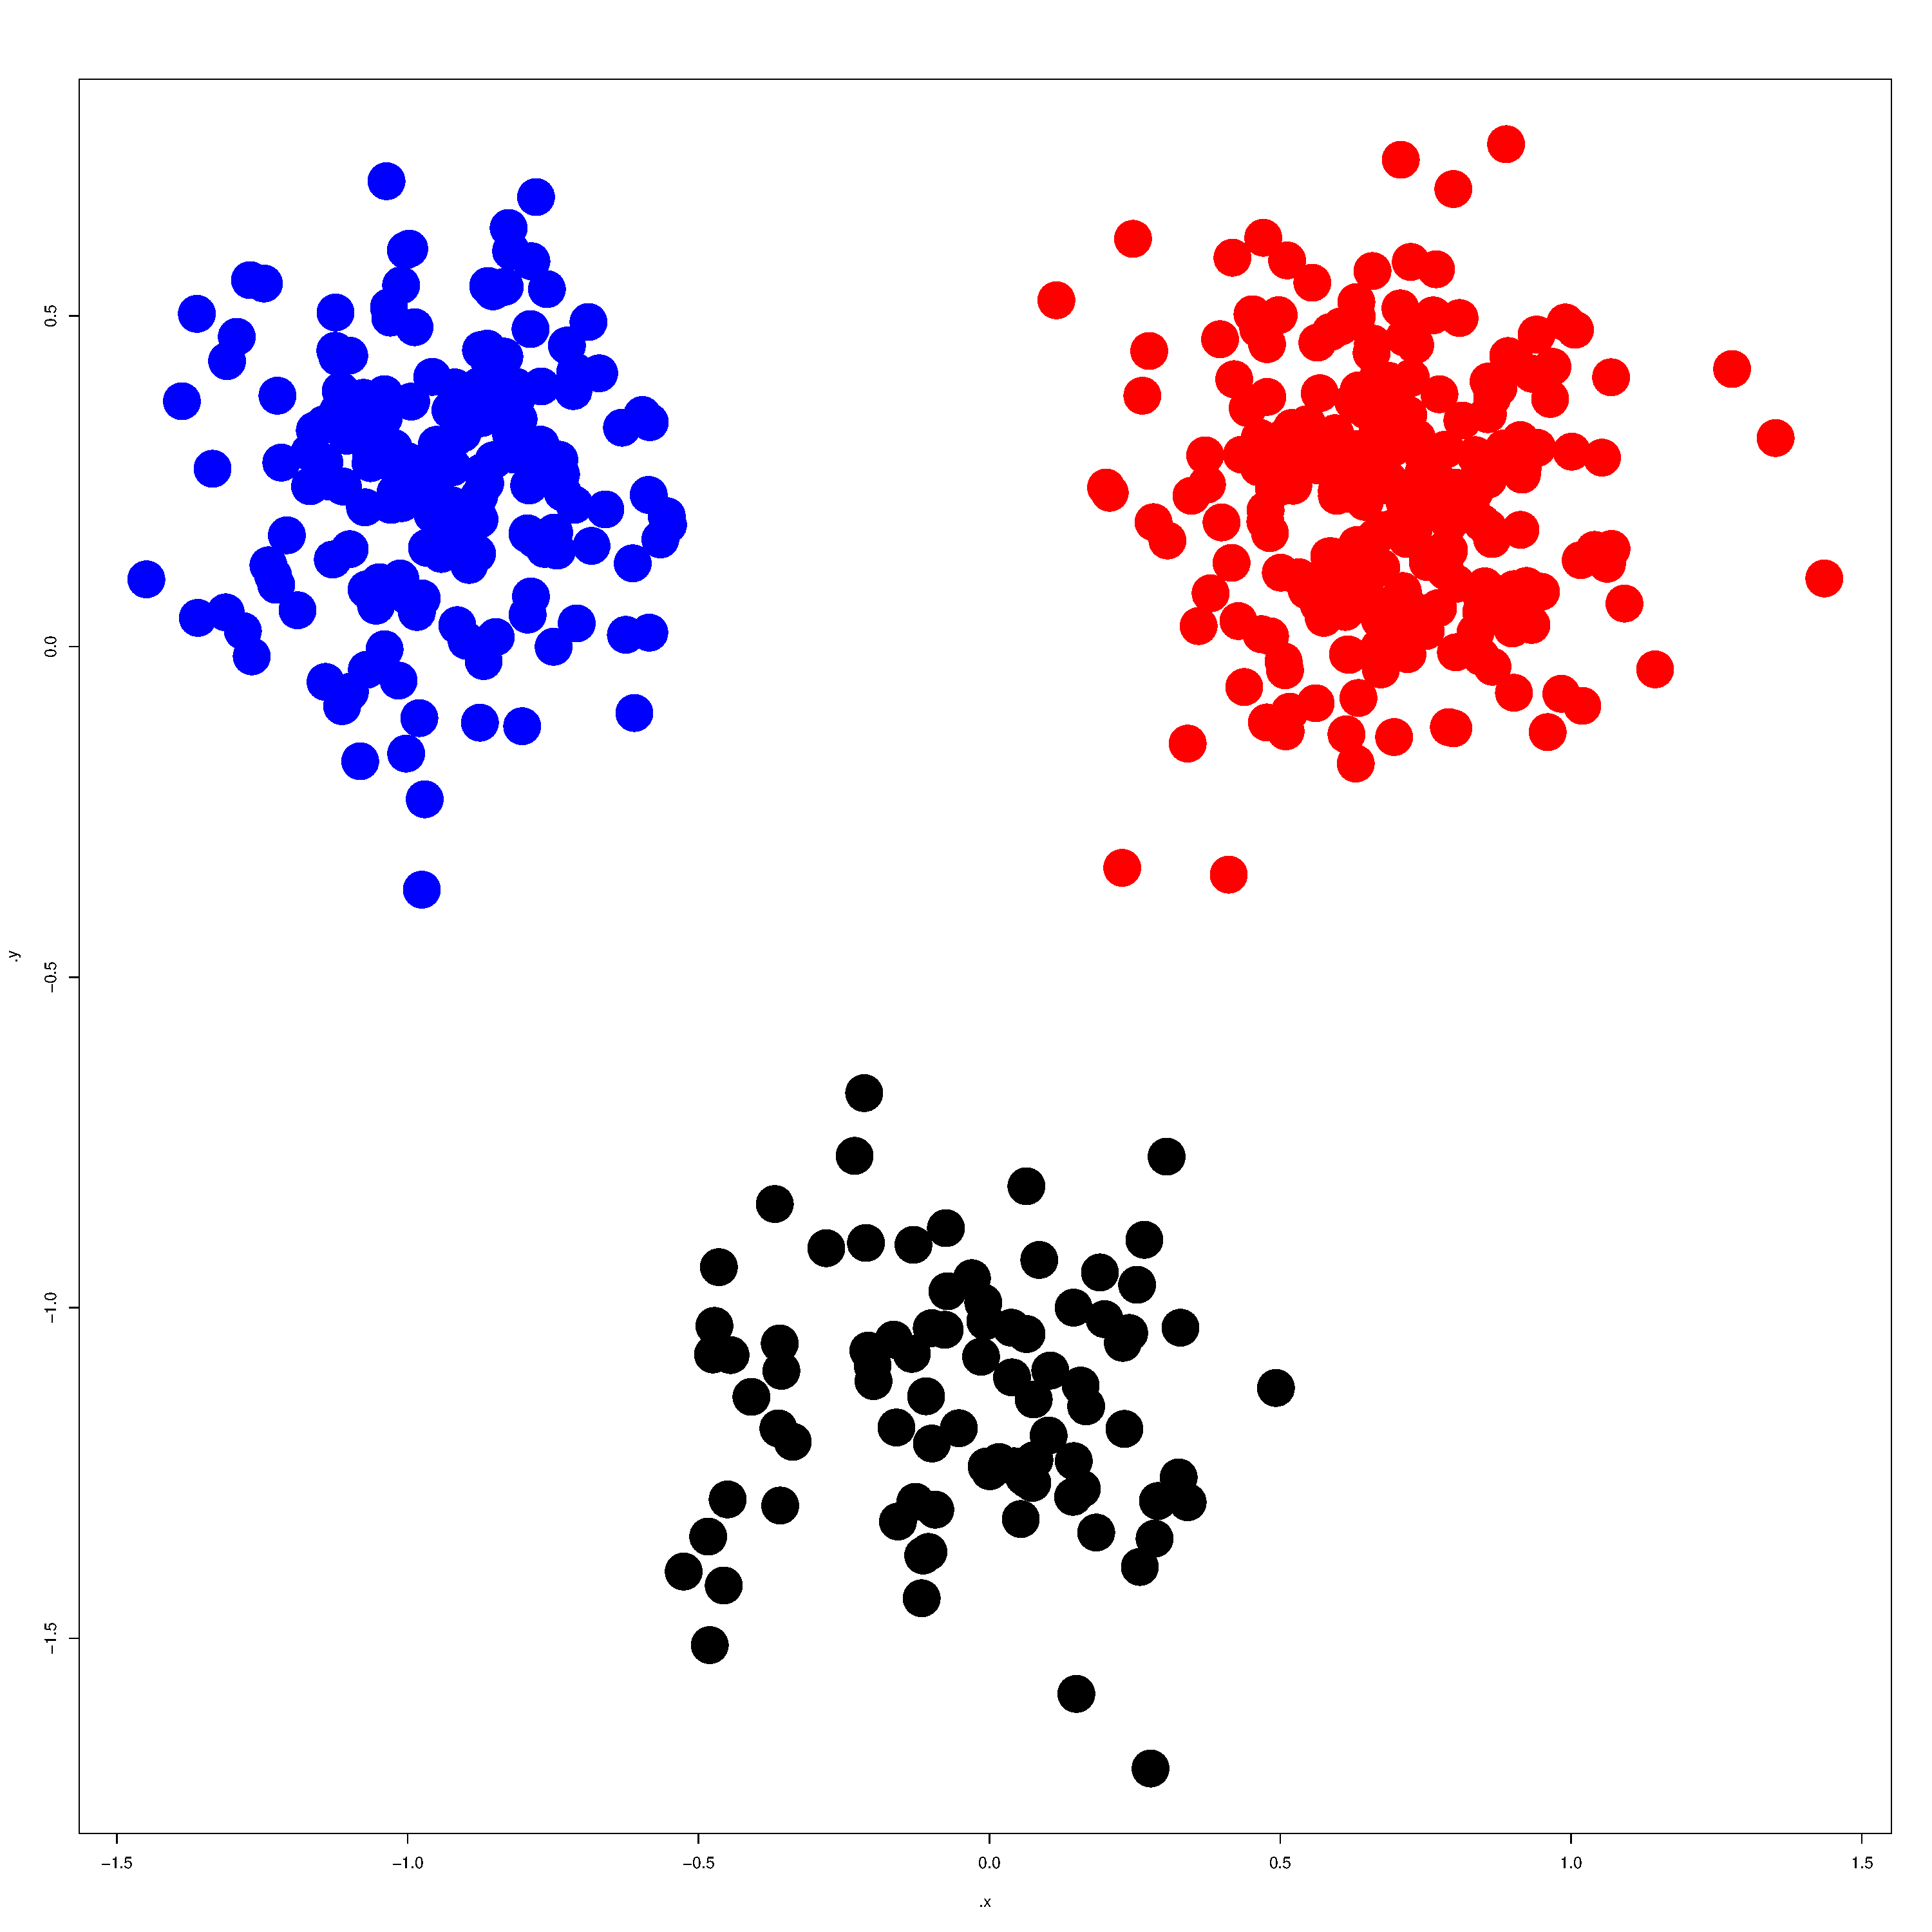
\includegraphics[height=2.5cm]{figures/clusters_expl.pdf}
        \caption{Matching class structure with visible blobs.}
    \end{subfigure}
    ~
    \begin{subfigure}[t]{0.45\textwidth}
	    \centering
        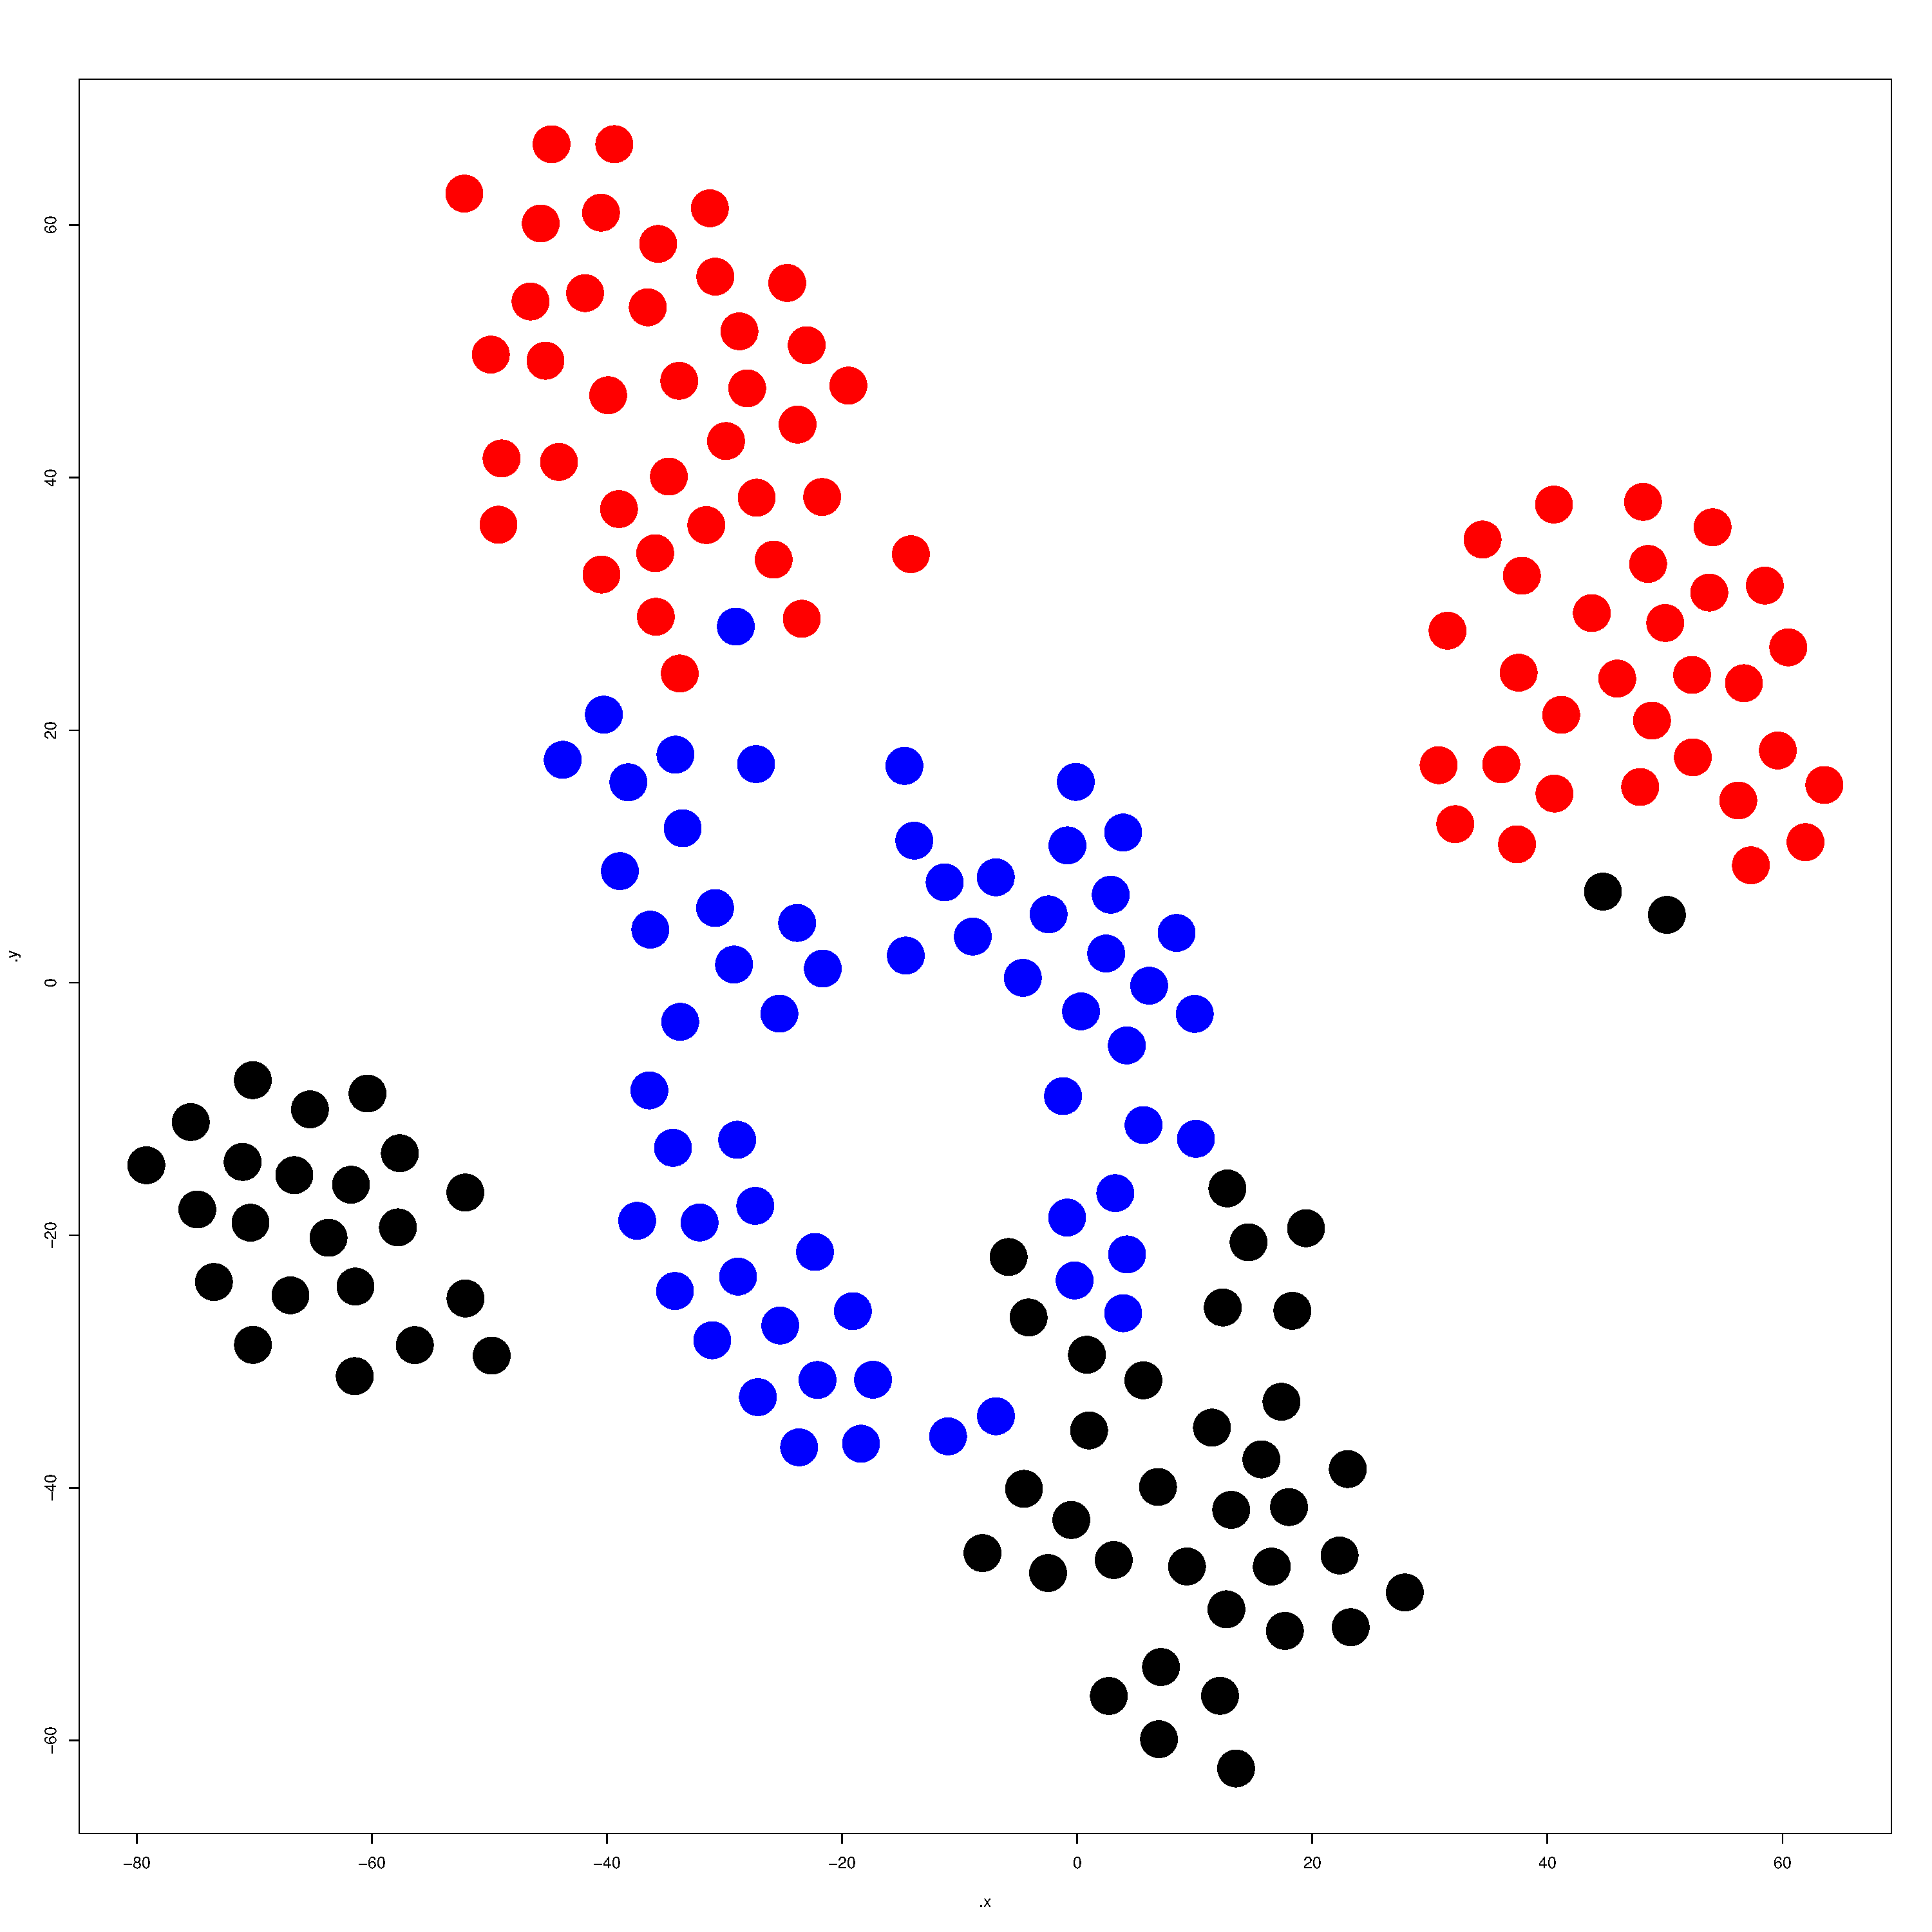
\includegraphics[height=2.5cm]{figures/clusters_expl_mismatch.pdf}
        \caption{A mismatch of class structure with visible blobs.}
    \end{subfigure}
    ~
    \begin{subfigure}[t]{0.45\textwidth}
	    \centering
        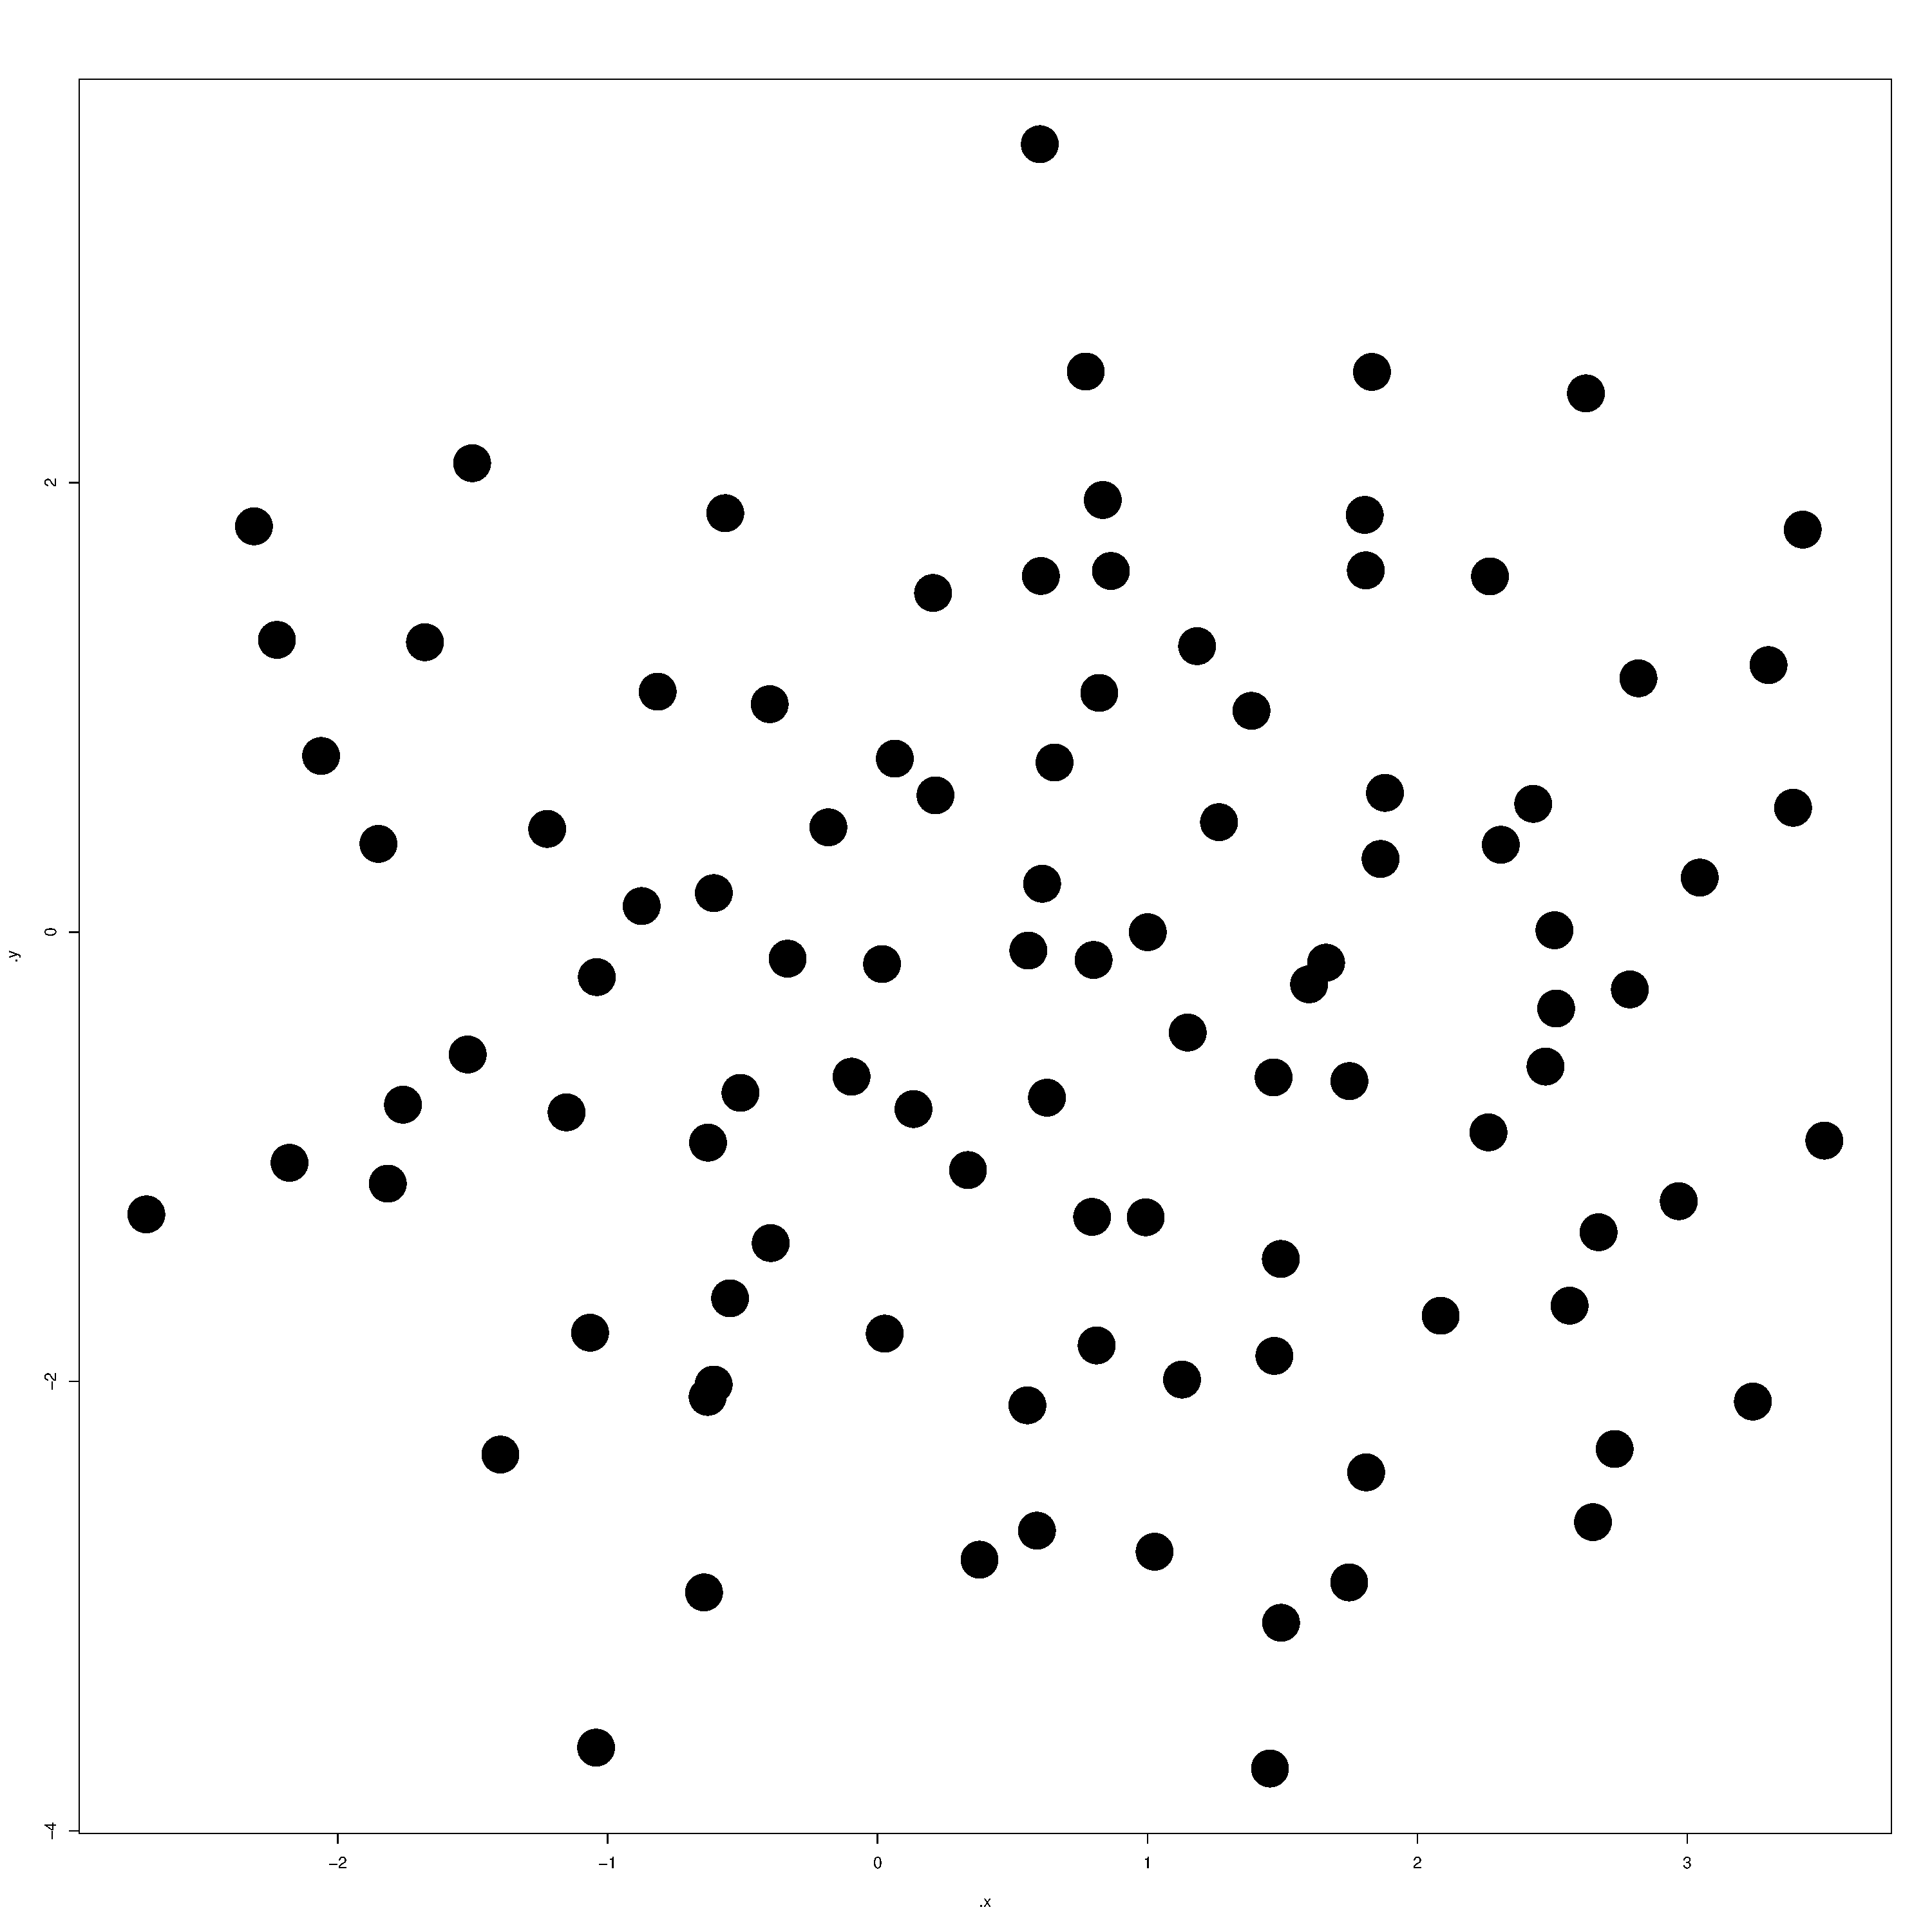
\includegraphics[height=2.5cm]{figures/blob_impl.pdf}
        \caption{An undistinguishable clutter of unlabeled data.}
    \end{subfigure}
    ~
    \begin{subfigure}[t]{0.45\textwidth}
	    \centering
        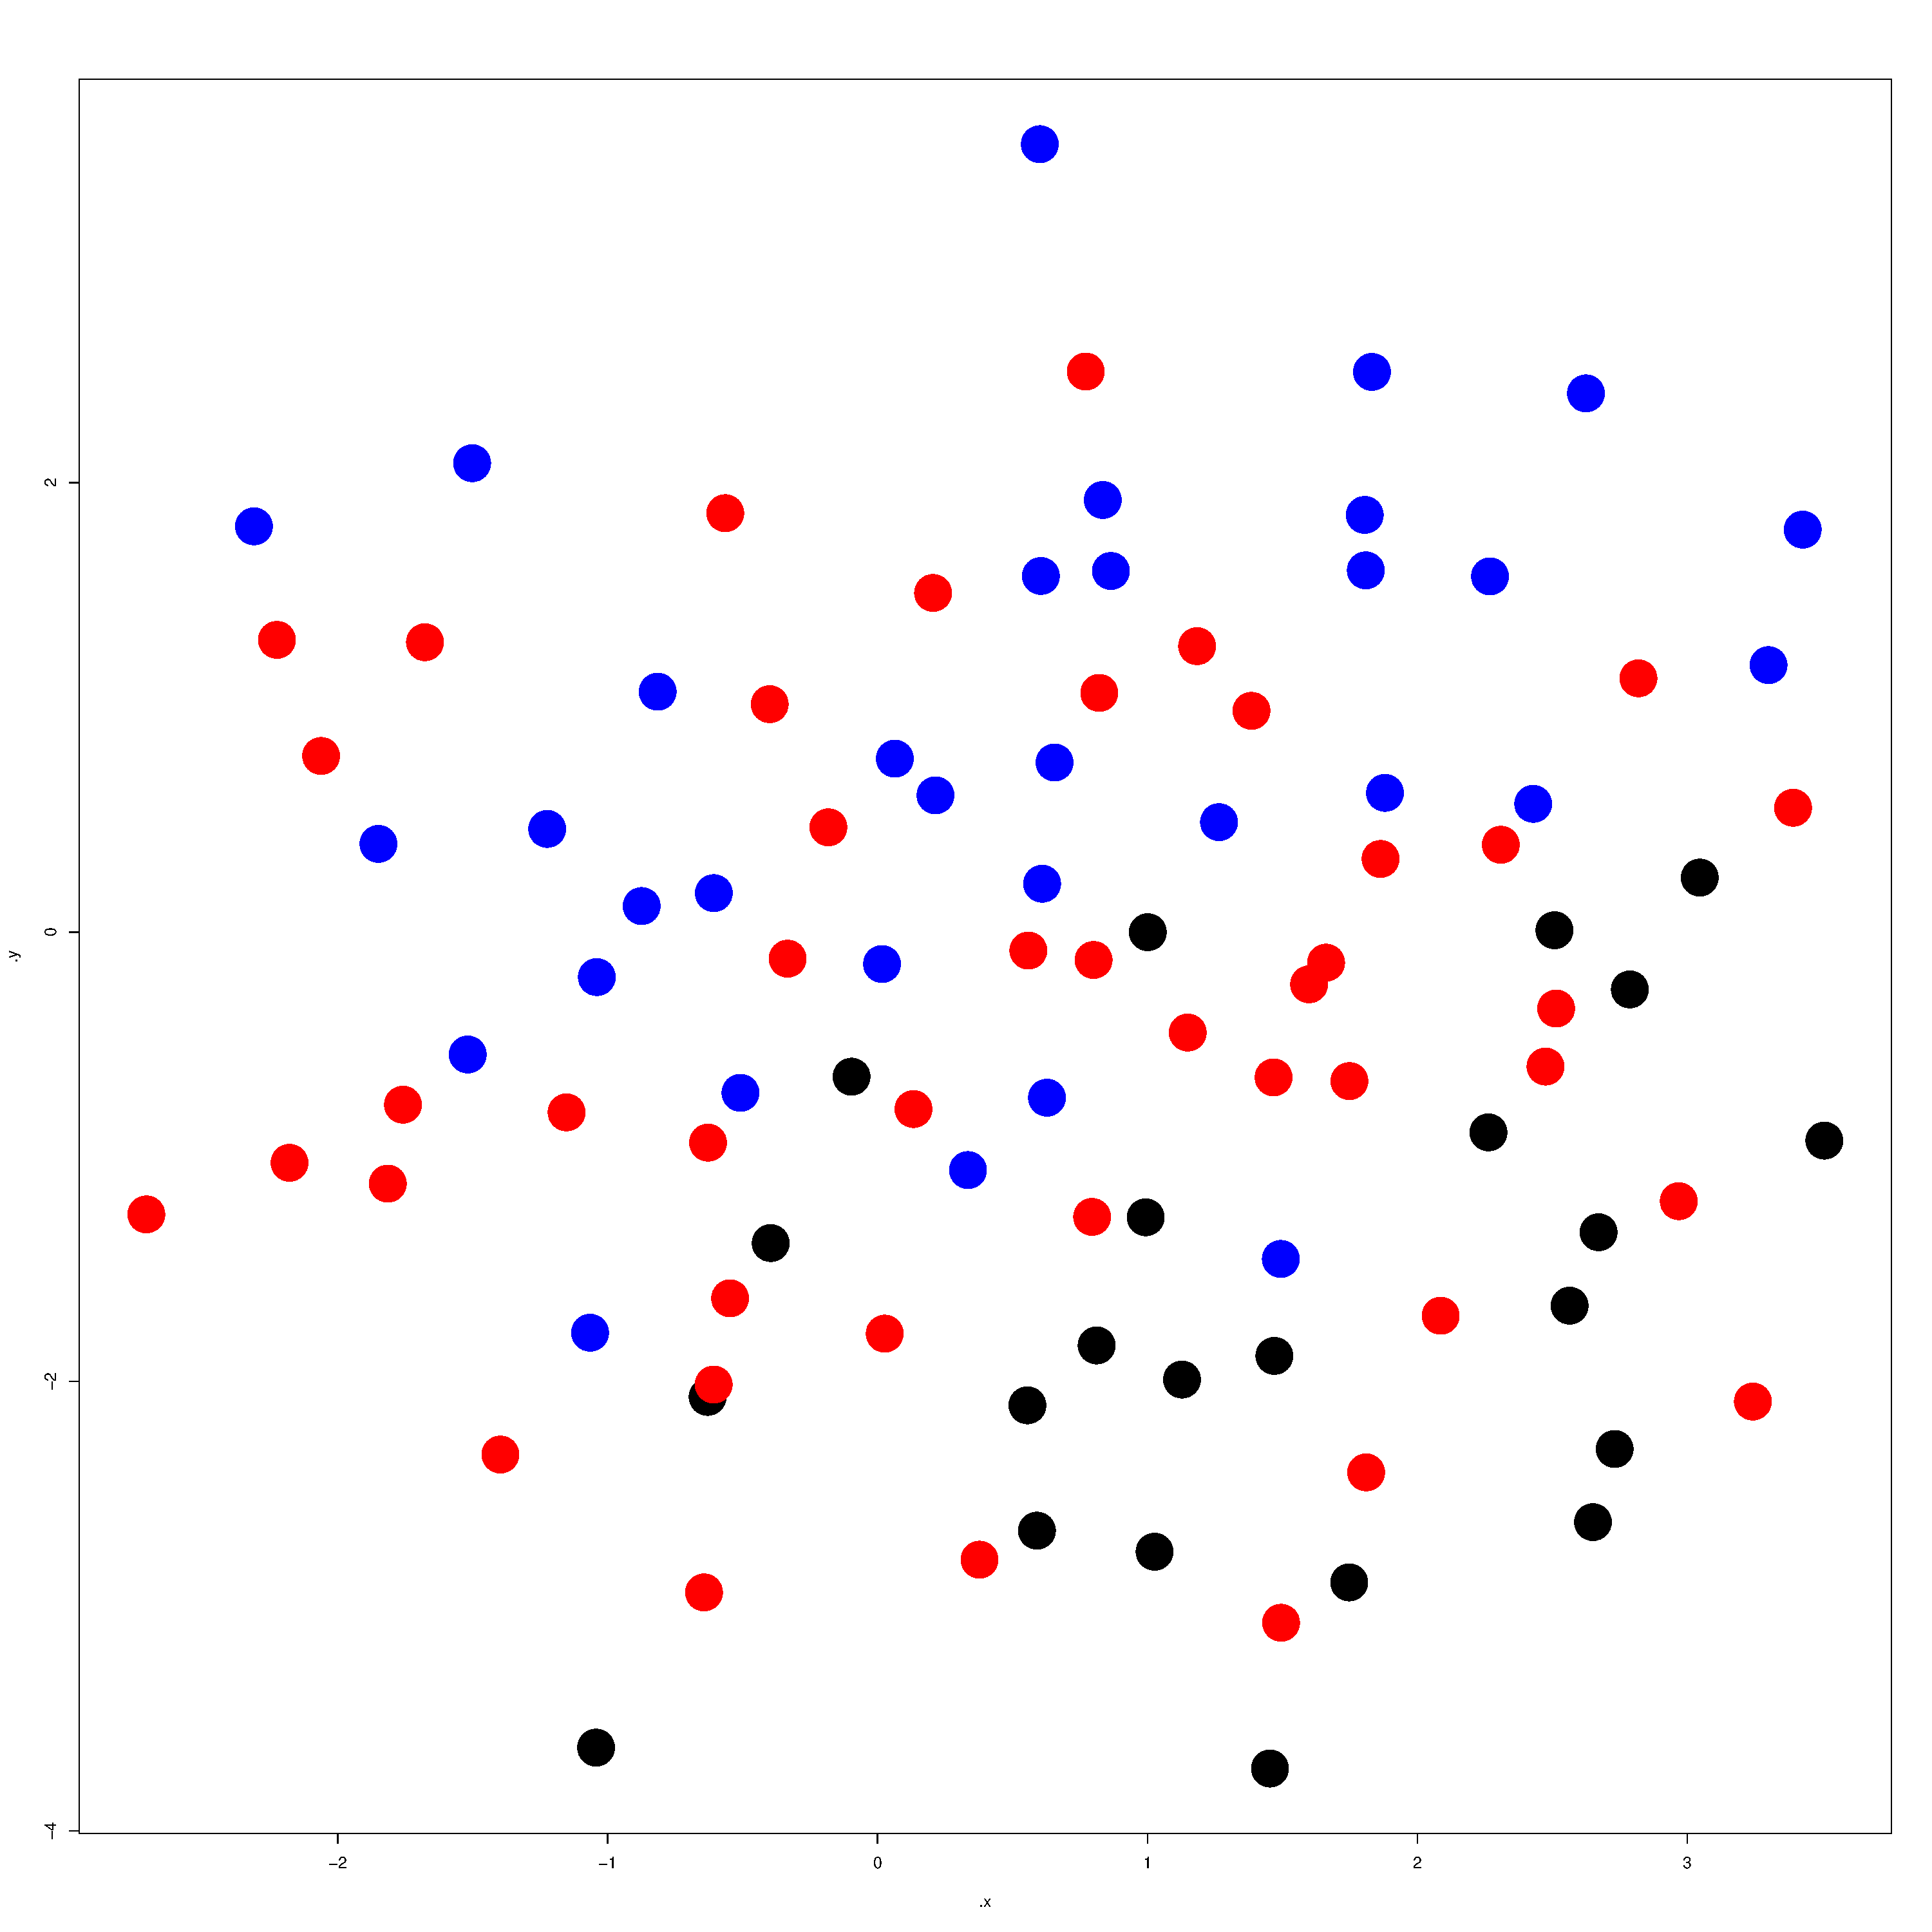
\includegraphics[height=2.5cm]{figures/blob_expl.pdf}
        \caption{An undistinguishable clutter of labeled data.}
    \end{subfigure}
	\caption
	[
	    Example scatterplots of dimensionally reduced data illustrating potential tasks related to checking cluster separability.
	]
	{
    	Example scatterplots of dimensionally reduced data illustrating potential tasks related to checking cluster separability. Cases (d) and (e) usually lead to refining \ac{DR}, visual encoding, or clustering algorithm choices and parametrizations.
	}
	\centering
	\label{app:drvistasks:fig:clusters}
\end{figure}

%-|-|-|-|-|-|-|-|-|-|-|-|-|-|-|-|-|-|-|-|-|-|-|-|-|-|-|-|-|-|-|-|-|-|-|-|-

\bstart{Name blobs} 
The {\it name blobs} task\index{task}, which we observed in fifteen usage examples, describes a person's intent to identify visually separable blobs of (monochrome) points in a scatterplot\index{visual encoding!scatterplot} of dimensionally reduced data\index{dimensionality reduction (DR)} and to assign meaning to these clusters. 
If blobs are visually separable in a low-dimensional projection, as shown in \autoref{app:drvistasks:fig:clusters}a, an analyst could assume that these blobs represent meaningful groups. 

\begin{quotation}
    In the {\sc TxtDocs} usage example, a journalist\index{journalism} (\ref{drvistasks:analyst:JS}) was interested in characterizing patterns of incidents reported by defense contractors during the Iraq war.
    Several thousand hard copy incident reports were scanned and subject to optical character recognition, resulting in an unstructured text file for each report.
    Each report was converted into a weighted vector of words, and the cosine similarity measure was computed between pairs of these vectors.
    The distances between vectors served as input to Glimmer \ac{MDS}\index{dimensionality reduction (DR)!multi-dimensional scaling (MDS)}~\cite{Ingram2009}, which generated a monochrome two-dimensional scatterplot\index{visual encoding!scatterplot} visual encoding\index{visual encoding} of the documents\index{document data}. 
    Overlaid on these points were the top weighted terms from their corresponding vectors.  
    
    The journalist\index{journalism} observed visible structure in this visual encoding\index{visual encoding}, and was able to identify clusters of incidents and their distinguishing features: the involvement of civilians, official dignitaries, or combatants, the presence and type of casualties, the locations, dates, and times of incidents, and whether the incident involved the use of weapons or vehicles.
\end{quotation}

\bstart{Match blobs and classes} 
If classes are available for color-coding the points and if visually separable blobs are visible as in \autoref{app:drvistasks:fig:clusters}b and \autoref{app:drvistasks:fig:clusters}c, a typical task\index{task} is to evaluate\index{evaluation} the match between blobs and class structure: that is, checking whether the colors match with the spatial structure in the layout.  

\begin{quotation}
    The {\sc MoCap} analyst (\ref{drvistasks:analyst:KA}), a machine learning\index{machine learning} researcher
    interested in building predictive motion capture models
    based on a dataset with given {\it class structure}. 
    Using forty-five carefully calibrated accelerometers, gyroscopes, and magnetometers, each attached to a part of the body of human subjects, he captured instances of human motion: walking, standing up, lying down, and so on. 
    Instances of the same motion were grouped together in the same class, and represented the ground truth class structure of his motion capture recordings.
    From these sensors, a large number of time-varying derived variables (approximately 25 per sensor) were recorded\index{time-oriented data}, resulting in datasets of approximately one thousand dimensions and approximately ten thousand recorded motions (points). 

    In usage example {\sc MoCap A}, \ref{drvistasks:analyst:KA} was interested in verifying that the classes of motion types formed visibly distinct blobs within the layout of points in a scatterplot\index{visual encoding!scatterplot}. 
    He reduced the data using linear \ac{PCA}\index{dimensionality reduction (DR)!principal component analysis (PCA)} or \ac{SFS}\index{sequential forward selection (SFS)} automatic filtering~\cite{Jain2000} to either two or three dimensions, then visualized the result in two-dimensional\index{visual encoding!scatterplot} or three-dimensional scatterplots\index{visual encoding!scatterplot!3D scatterplot}, with points colored according to their motion class. 
    However, regardless of the \ac{DR}\index{dimensionality reduction (DR)} technique used, the colored blobs did not unambiguously match the class structure of points. 
\end{quotation}

Another common case is that analysts start out with exploring an unlabeled dataset and then uses a clustering algorithm\index{algorithms!clustering} to suggest a certain class structure. 
In this case, the analyst starts out with an initial {\it name blob} task\index{task} and then engages in {\it matching} the suggested class labels with the visible point layout (six usage examples). 
Automatic labeling by way of a clustering algorithm\index{algorithms!clustering} is therefore used to facilitate the detection of clusters that exist in the high-dimensional space.

\begin{quotation}
    Before the {\sc Music} analyst (\ref{drvistasks:analyst:JB}) shifted her focus to finding and grouping important dimensions as described above (usage example {\sc Music B}), she was interested in identifying and naming clusters of listeners (usage example {\sc Music A}).
    Her particular interest was to cluster people into groups with similar listening behavior.
    She hypothesized several groups a priori, such as people who listen to the same music repetitively vs.~people who listen to new music, or people who listen during the day vs.~those who listen at night. 
    She used \ac{PCA}\index{dimensionality reduction (DR)!principal component analysis (PCA)} to reduce the dataset, which she plotted using monochrome scatterplots\index{visual encoding!scatterplot}.
    Unable to perceive meaningful cluster structure in the monochrome plot, she applied a $k$-means clustering\index{algorithms!clustering} to generate colored scatterplots\index{visual encoding!scatterplot} of the low-dimensional data. However, even after repeated changes to the size of the $k$ parameter, the number of clusters, she was not able to identify any meaningful cluster structure. 
    She gave up on her clustering\index{algorithms!clustering} endeavors and switched to learning about her dimensions as described above.
\end{quotation}

\bstart{Refining DR, visual encoding, and clustering} 
Low-dimensional projections rarely represent the full details of a high-dimensional dataset\index{high-dimensional data} and different algorithmic\index{algorithms} choices and parametrizations\index{algorithms!parametrization of} lead to different visual encodings\index{visual encoding} of the data.
In practice, identifying separable clusters has therefore to be seen as a spectrum between seeing no visible class structure at all, as in \autoref{app:drvistasks:fig:clusters}d and \autoref{app:drvistasks:fig:clusters}e, to clearly seeing separable point clusters, as in \autoref{app:drvistasks:fig:clusters}a and \autoref{app:drvistasks:fig:clusters}b. 
A very common task\index{task} in this spectrum is to iteratively {\it refine \ac{DR}, visual encoding, and/or clustering}\index{visual encoding} algorithms\index{algorithms!clustering} by selecting alternative choices and parametrizations\index{algorithms!parametrization of}, with the goal of seeing clearer separability.
In the following usage example an analyst tried different \ac{DR}\index{dimensionality reduction (DR)} algorithms\index{algorithms} and parametrizations\index{algorithms!parametrization of}, toward the goal of identifying clusters:

\begin{quotation}
    In the {\sc Concept} usage example, \ref{drvistasks:analyst:HY}'s goal was to visualize research concept clusters, to be used by life science researchers, allowing her to identify higher-level concept clusters and other researchers working in areas related to their own. 
    The dataset stemmed from a database of all life science researchers in which each researcher is represented by a set of ranked research concepts. 
    Overall there are twenty thousand concepts, including terms such as ``DNA'' or ``cancer''. 

    As her eventual goal was to build a helpful visualization tool, her immediate task\index{task} was to identify groups of concepts. 
    To do so, she computed a distance matrix of concepts based on their co-occurrence in the researcher database. 
    For visualization, this matrix was then used as input first to classical \ac{MDS}\index{dimensionality reduction (DR)!multi-dimensional scaling (MDS)} and then to Glimmer \ac{MDS}\index{dimensionality reduction (DR)!multi-dimensional scaling (MDS)}~\cite{Ingram2009}, the latter with a variety of parametrizations\index{algorithms!parametrization of}. 
    Yet, no approach revealed any meaningful visible cluster structure, but only an undifferentiated clutter of points.
    The analyst finally decided that the non-existence of visible separation is not just an algorithmic\index{algorithms} artifact. 
    Trying different algorithmic\index{algorithms} choices and parametrizations\index{algorithms!parametrization of} gave her a certain degree of confidence in her decision.
\end{quotation}

Judging whether non-visible/visible cluster structure correctly reflects the high-dimensional data\index{high-dimensional data} or whether it stems from algorithmic\index{algorithms} artifacts is a major challenge we observed. 
To address this challenge, all our interviewees concerned with checking point clusters, including the {\sc TxtDocs} (\ref{drvistasks:analyst:JS}), {\sc MoCap B} (\ref{drvistasks:analyst:KA}), and {\sc Music A} (\ref{drvistasks:analyst:JB}) usage examples described above, engaged to some degree in {\it refining}. 

Abstractly, this central question can be phrased in terms of whether the presence or absence of visible cluster structure is a {\it false/true negative/positive} result.
An undifferentiated clutter of all points is the most common situation, which could be either indicative of a false negative or a true negative.
If an analyst suspects a {\it false negative}, she will probably decide to refine algorithmic\index{algorithms} choices and/or parametrizations\index{algorithms!parametrization of}; the analyst might, for instance, decide to use non-linear \ac{DR}\index{dimensionality reduction (DR)} techniques instead of linear techniques, or to use a \ac{SPLOM}\index{visual encoding!scatterplot!scatterplot matrix (SPLOM)} instead of two-dimensional scatterplots\index{visual encoding!scatterplot}. 
The goal of this refinement is to move incrementally from few or no visible clusters toward more visible structure. 

Alternatively, an analyst may consider an undifferentiated clutter of points to be a {\it true negative}, meaning that there is no cluster structure in the dataset. 
This consideration often occurs after an analyst has tried many different technique and parameterization choices. 
The {\sc Concept} usage example (\ref{drvistasks:analyst:HY}) is an example where the analyst eventually gave up. 

When clear clusters are visible, an analyst will often declare victory, as the spatial layout indicates a {\it true positive}. 
In contrast, there may be instances when an analyst mistrusts the visible structure, attributing it to an artificial algorithmic\index{algorithms} artifact (a {\it false positive}). 
These situations are probably less common; we observed none in our study.

%-------------------------------------------------------------------------

\subsubsection{DR for Algorithmic Input}
\label{app:drvistasks:dritw:taxonomy:algo}

%-------------------------------------------------------------------------

While all of the above tasks\index{task} were about using \ac{DR}\index{dimensionality reduction (DR)} for the purpose of data analysis and visualization, another purpose of \ac{DR}\index{dimensionality reduction (DR)} is algorithmic input\index{algorithms!algorithmic input}, a common case in machine learning\index{machine learning}.
We identified seven usage examples in which \ac{DR}\index{dimensionality reduction (DR)} was used for preparing a dataset for algorithmic input\index{algorithms!algorithmic input}, reflected by the right-most branch of \autoref{fig:dritw-taxonomy-2}. 
In these usage examples, the goal is to reduce the dataset's dimensions in order to improve the performance of downstream algorithmic\index{algorithms} processing, and to make a predictive model more reliable, robust and accurate by avoiding the curse of dimensionality~\cite{Bellman1961}. 
This task\index{task} is well-described in the machine learning\index{machine learning} community~\cite{Murphy2012}. 

Earlier, we described the {\sc MoCap A} usage example (\ref{drvistasks:analyst:KA}), where the analyst strived to {\it match blobs with classes} of motion types in two-dimensional\index{visual encoding!scatterplot} or three-dimensional scatterplots\index{visual encoding!scatterplot!3D scatterplot}.
In a larger context, his ambitions to visually analyze the data were one step toward his ultimate goal of building a motion classifier\index{algorithms!classification}, which involved performing \ac{DR}\index{dimensionality reduction (DR)} for the purpose of algorithmic input\index{algorithms!algorithmic input}: 

\begin{quotation}
    In the {\sc MoCap B} usage example, \ref{drvistasks:analyst:KA} wanted to use his motion capture dataset to train supervised motion classification algorithms\index{algorithms!classification}.
    Once again he used \ac{PCA}\index{dimensionality reduction (DR)!principal component analysis (PCA)} or \ac{SFS}\index{sequential forward selection (SFS)} to reduce the number of dimensions in his dataset. 
    After manually inspecting scree plots\index{visual encoding!scree plot}, he selected roughly thirty dimensions to train a supervised motion classification algorithm\index{algorithms!classification}. 
    Despite his failed attempt to visually verify groups in his data (usage example {\sc MoCap A}), he was sufficiently satisfied by the performance of his classifier\index{algorithms!classification} trained with the 30-dimensional reduced data that he considered these groups to be a true positive result. 
    His results from {\sc MoCap A} can therefore be seen as a false negative.
\end{quotation}

%-------------------------------------------------------------------------

\subsubsection{High-dimensional Data Analysis and DR}
\label{app:drvistasks:dritw:taxonomy:disc}

%-------------------------------------------------------------------------

Although \ac{DR}\index{dimensionality reduction (DR)} was the focus of our investigation, many of the tasks\index{task} we found might be also conducted without the direct need for the application of \ac{DR}\index{dimensionality reduction (DR)} algorithms\index{algorithms}. 
The only tasks\index{task} we found where \ac{DR}\index{dimensionality reduction (DR)} is inherently necessary for are tasks\index{task} about new dimensions. 
All other tasks\index{task} can be seen as a subset of general high-dimensional data\index{high-dimensional data} analysis for which we found instances that coexisted with \ac{DR}\index{dimensionality reduction (DR)} usage. 
Naturally, there will be many other abstract tasks\index{task!task abstraction} if the scope is broadened to high-dimensional data\index{high-dimensional data} analysis. We see our work as a first step toward a better understanding of those tasks\index{task} ``in the wild''\index{evaluation!in the wild}.

We found that the question whether \ac{DR}\index{dimensionality reduction (DR)} will or will not be a valuable tool for the analysis of a high-dimensional dataset\index{high-dimensional data} is often not straightforward for an analyst or designer to answer. 
In particular, we observed two instances in which our interviewees attempted to use \ac{DR}\index{dimensionality reduction (DR)} after our initial interview, but eventually realized that no \ac{DR}\index{dimensionality reduction (DR)} was needed for the purpose of accomplishing the analysis of their high-dimensional data\index{high-dimensional data}. 
In the following usage example, sensitivity analysis\index{sensitivity analysis} alone without \ac{DR}\index{dimensionality reduction (DR)}, for instance, was the actual solution:

\begin{quotation}
    The {\sc FishPop} usage example involves a biologist\index{fisheries sciences} (\ref{drvistasks:analyst:CH}) whose goal is to provide recommendations about balancing the risks of overfishing with commercial and private fishing interests.
    She compares and evaluates several different models that simulate the behavior of fish populations.
    All these models take a set of input parameters, such as carrying capacity and productivity, typically generated via regular sampling in the space of possible parameter configurations. 
    The output of these models is an indication of the probability that a fish population will die out.
    Her main concern is sensitivity analysis\index{sensitivity analysis}: checking whether small changes in input dimensions lead to small or large changes in output dimensions. 
    Sensitivity is a main aspect of recommending one model over another. 
    Although she experimented with \ac{DR}\index{dimensionality reduction (DR)} algorithms\index{algorithms} after our initial interview, she ultimately resolved that no existing unmodified \ac{DR}\index{dimensionality reduction (DR)} technique was appropriate or even necessary for her dataset and task\index{task} at hand, and did not pursue this line of analysis further.
\end{quotation}

We include this discussion here to illustrate that some analyses may not benefit from \ac{DR}\index{dimensionality reduction (DR)}. 
While many analysts and designers might be quick to assume a need for \ac{DR}\index{dimensionality reduction (DR)}, it may be inappropriate or even present confounding results. 
Our suite of \ac{DR}\index{dimensionality reduction (DR)}-related tasks\index{task} offers more clarity and guidance for those who are facing such decisions at the interplay of high-dimensional data\index{high-dimensional data} analysis and \ac{DR}\index{dimensionality reduction (DR)}.

%-------------------------------------------------------------------------

\subsection{Challenges}
\label{app:drvistasks:dritw:challenges}

%-------------------------------------------------------------------------

We observed several challenges encountered by people when using \ac{DR}\index{dimensionality reduction (DR)} for their data analysis endeavors. 
Their struggles are of interest as stumbling blocks in daily practice that affected multiple people, and are not necessarily a sign that there is no solution in the technical literature. 
We discuss two of them in detail: the need for \ac{DR}\index{dimensionality reduction (DR)} that explicitly handles different groups of dimensions, and the need for nonlinear techniques that support unmapping new to old dimensions. 

\bstart{DR with groups of dimensions}
{\sc NPAlgo} (\ref{drvistasks:analyst:KLB}), {\sc StrucGen} (\ref{drvistasks:analyst:JWB}), and {\sc FishPop} (\ref{drvistasks:analyst:CH}) were some of the usage examples that involved comparing  groups of dimensions. 
Some analysts, such as in the {\sc FishPop} usage example, perform this comparison and have no need for \ac{DR}\index{dimensionality reduction (DR)} at all, and sensitivity analysis\index{sensitivity analysis} alone may be the appropriate task\index{task} for them to perform. 
However, other analysts have an additional need to reduce the dimensions of their data. 
This combination does not inherently result in a problem. 
For instance, the {\sc StrucGen} analyst (\ref{drvistasks:analyst:JWB}) was able to meet his needs with \ac{DR}\index{dimensionality reduction (DR)} in the form of filtering; he reduced the number of dimensions in each of his three groups of dimensions independently from one another, and then compared the reduced groups. 

However, in the {\sc NPAlgo} usage example (\ref{drvistasks:analyst:KLB}), which involved a predictive model of NP-hard algorithms\index{algorithms}, groups of dimensions possessed an inherent and important dependency on one another.
In particular, the analyst observed cases where a specific input dimension contributes very little to the overall variance nevertheless had a huge impact on the output dimension run time; converse cases were also observed. 
In these cases, it is not useful to apply a \ac{DR}\index{dimensionality reduction (DR)} technique solely on the input dimensions, because the crucial information about the intrinsic relation of the input dimensions to the output dimensions is not considered in the \ac{DR}\index{dimensionality reduction (DR)} computation. 
Neither can a synthetic \ac{DR}\index{dimensionality reduction (DR)} be run simultaneously on both input and output dimensions.
The importance of original input variables with regard to their influence on the output variable is not acknowledged by common \ac{DR}\index{dimensionality reduction (DR)} metrics, such as variance as in \ac{PCA}\index{dimensionality reduction (DR)!principal component analysis (PCA)}, or stress as in \ac{MDS}\index{dimensionality reduction (DR)!multi-dimensional scaling (MDS)}. 
In general, this problem may occur in situations with $n$ groups of dimensions and an arbitrary arrangement of dependencies between these groups. 

A first approach toward solving this problem was outlined by \citet{Gerber2009}. Their focus is on continuous high-dimensional input manifolds that map to one output variable. 
In brief, the high-dimensional input space is partitioned into monotonic areas that are separately projected to two dimensions using \ac{PCA}\index{dimensionality reduction (DR)!principal component analysis (PCA)}. 
These two-dimensional input parts can then be plotted together with the one output dimension in three dimensions. 
This approach allows people to visually explore relations between a group of multiple input dimensions and one output dimension. 
This approach, however, does not per se provide a \ac{DR}\index{dimensionality reduction (DR)} technique that would handle interdependent dimensional groups appropriately as needed by the {\sc NPAlgo} analyst (\ref{drvistasks:analyst:KLB}). 
A statistical approach toward that goal is \ac{CCA}\index{canonical correlation analysis (CCA)}, a method for identifying highly-correlated linear combinations of both input and output dimensions~\cite{Hotelling1936}. 
As with \ac{PCA}\index{dimensionality reduction (DR)!principal component analysis (PCA)}, \ac{CCA}\index{canonical correlation analysis (CCA)} is limited to producing linear projections of the input data.
Furthermore, the dimensionality of \ac{CCA}\index{canonical correlation analysis (CCA)} projections can be no greater than the smaller dimensionality of the input and output groups. 
In case of the {\sc NPAlgo} (\ref{drvistasks:analyst:KLB}), reducing the input space to one linear dimensions would not have been satisfying for the analyst. 
We see ample opportunities for future technical contributions in this set of challenges. 

\bstart{Non-linear unmapping}
Our study emphasized that some analysts are interested in both {\it old} and {\it new} dimensions at the same time.
Identifying these relationship often takes a top-down approach: a synthetic \ac{DR}\index{dimensionality reduction (DR)} algorithm\index{algorithms} is used and the analyst tries to {\it unmap} these new dimensions to their old dimensions, such as in the {\sc Music B} example (\ref{drvistasks:analyst:JB}). 
Alternatively, some analysts take a bottom-up approach, in which they manually {\it group correlated} dimensions together and then aggregate these groups into new dimensions, such as the {\sc BoatAct} example (\ref{drvistasks:analyst:CM}). 
When analysts performed this task\index{task}, they used linear techniques such as \ac{PCA}\index{dimensionality reduction (DR)!principal component analysis (PCA)} because there is no support for unmapping with any nonlinear \ac{DR}\index{dimensionality reduction (DR)} technique. 

However, in cases such as usage example {\sc Music B}, the \ref{drvistasks:analyst:JB} would have benefited from a more powerful nonlinear \ac{DR}\index{dimensionality reduction (DR)} technique. 
The analyst wanted to account for as much of the variance of the original data as possible with a small number of new dimensions, while at the same time maintaining an understandable semantic mapping between old and new dimensions. 
With linear \ac{DR}\index{dimensionality reduction (DR)} techniques, this criterion was only partially satisfied, due to their limited power.

While we are well aware that unmapping non-linear combinations is a difficult undertaking, even a partial solution would improve the state of the art. 
Interactive visualization may well be a fruitful avenue to pursue, for helping people explore a complex non-linear dimensional mapping space.

\bstart{Other challenges}
Analysts reported several other challenges that have been previously identified in the literature, including \ac{DR}\index{dimensionality reduction (DR)} scalability issues with large datasets \cite{Brandes2007,Ingram2009}, extreme ratios between dimensions and points with many more dimensions than points \cite{Cunningham2008,West2003}, and the existence of categorical dimensions in the data \cite{Friendly2000,Greenacre2006}.  

We also found supporting evidence for our previous hypothesis on the need for guidance~\cite{Ingram2010}. 
While all of the analysts were experts in their own domain, thirteen analysts indicated a lack of expertise in the mathematical implications of \ac{DR}\index{dimensionality reduction (DR)} techniques, while only eight analysts indicated deep understanding.

%-------------------------------------------------------------------------

\subsection{Benchmarks}
\label{app:drvistasks:dritw:benchmarks}

%-------------------------------------------------------------------------

One of our initial motivations for this project related to an apparent gap between benchmark \ac{DR}\index{dimensionality reduction (DR)} datasets used in different communities. 
In this section, we discuss this gap and show how our work adds clarification by defining tasks\index{task}.

A canonical \ac{DR}\index{dimensionality reduction (DR)} benchmark often referred to in the machine learning\index{machine learning} literature is the synthetic {\it Swiss roll} dataset that is a simple two-dimensional strip rolled into a three-dimensional spiral shape. 
It shows off the capabilities of the {\it manifold following} non-linear \ac{DR}\index{dimensionality reduction (DR)} techniques such as Isomap~\cite{Tenenbaum2000} and Laplacian Eigenmaps~\cite{Belkin2001}, which assume that the high-dimensional data\index{high-dimensional data} lies on a densely sampled manifold that can be ``unrolled'' to a lower-dimensional representation. 
In contrast, cluster datasets of the type shown in \autoref{app:drvistasks:fig:clusters} typify those described by \citet{Sedlmair2012a}. 
Interestingly, these cluster datasets appear to completely violate the manifold assumption. 
We were initially skeptical that methods optimized for manifold datasets would work well on other datasets, and wondered about the contexts in which these datasets were representative of analysts' practices and needs.

Our field work sheds light on this question: both benchmark dataset types are represented by real-world scenarios, but these scenarios have very different underlying tasks\index{task} and associated assumptions. 
In particular, the assumption of a dataset lying on a densely sampled, single smooth manifold is strongly tied to the task\index{task} of {\it naming new dimensions}. 

We note that none of our interviewed analysts chose to apply manifold techniques; the two usage examples where these techniques were applied ({\sc BRDF, Faces}) were from the literature~\cite{Matusik2003,Tenenbaum2000}. 
In instances of the {\it name new dimensions} task\index{task} that emanated from our interviews (such as {\sc Concept} / \ref{drvistasks:analyst:HY} or {\sc Music B} / \ref{drvistasks:analyst:JB}) it was not clear that the assumption of a smooth manifold was met by the data.
In all other usage examples, the task\index{task} itself did not align with manifold assumptions.

We now elaborate further on the relationship between these tasks\index{task} and \ac{DR}\index{dimensionality reduction (DR)} algorithm\index{algorithms} assumptions to provide guidance to visualization practitioners.

\bstart{Densely sampled} 
Manifold techniques assume densely sampled data. 
However, analysts may not always be sure if their datasets meet the assumptions of a densely sampled manifold. 
We derived two criteria for understanding when a dataset is likely to qualify as a densely sampled manifold. 
First, all dimensions should be numerical and continuous, which negates any datasets containing categorical dimensions; the survey datasets from the {\sc Concept, Music} (\ref{drvistasks:analyst:HY}), and {\sc BoatAct} (\ref{drvistasks:analyst:CM})
usage examples, for instance, violate this assumption. 
Second, the dataset should be generated by a process that has the characteristics of continuous sampling. 
For example, 
in the {\sc MoCap} usage example (\ref{drvistasks:analyst:KA}), sensors measured body part motion over small time intervals; however, the analyst's tasks\index{task} did not include {\it naming new dimensions}, but rather {\it matching blobs and classes} and reducing the data for {\it algorithmic input}\index{algorithms!algorithmic input}.
Real-world measurements are a common case for manifolds, but manifolds may exist elsewhere, such as in the {\sc NPAlgo} usage example (\ref{drvistasks:analyst:KLB}), where the regularly changing values reflected algorithm\index{algorithms} parameters. 

\bstart{Single vs. multiple manifolds} 
In addition to densely sampled data, the classical {\it Swiss Roll} manifold unrolling use case comes with a further assumption: the data resides on a {\it single manifold}. 
Formally, the data distribution along all continuous dimensions needs to be homogeneous, rather than heterogeneous or clumpy. 
The {\it Swiss Roll} benchmark dataset is the canonical example for a single manifold; here the associated task\index{task} is one of carefully unrolling the single manifold. 
Clearly, this assumption matches only with the needs of analysts who perform the {\it name new dimensions} task\index{task}. 
In particular, such assumptions are less likely to be appropriate for tasks\index{task} involving point clusters. 
Point clusters may exist due to a non-uniform distribution of samples on a single manifold.
Alternatively, clusters may represent samples taken from multiple different manifolds. 
The data from the {\sc MoCap} example (\ref{drvistasks:analyst:KA}) is an instance where a multiple manifold structure is likely, with one densely sampled manifold per class of movement type. 
The machine learning\index{machine learning} community has noted the instability of older single manifold algorithms~\cite{Balasubramanian2002,VanderMaaten2009}\index{algorithms}, and newer techniques such as \ac{t-SNE}\index{dimensionality reduction (DR)!t-distributed stochastic neighbor embedding (t-SNE)}~\cite{VanderMaaten2008} have been proposed for identifying multiple manifolds, thus supporting tasks\index{task} relating to point clusters. 
However, the question of whether a dataset reflects the result of dense sampling along continuous dimensions remains.

%-------------------------------------------------------------------------

\subsection{Discussion}
\label{app:drvistasks:dritw:discussion}

%-------------------------------------------------------------------------

Our work provides a synthesis description of \ac{DR}\index{dimensionality reduction (DR)}-related tasks\index{task} that is both accessible to a visualization audience and grounded from a systematic study of real-world human behavior. 
In particular, we emphasize a differentiation between tasks\index{task} involving {\it point clusters} and those involving {\it dimensions}, the idea of {\it false/true positive/negative} groups of points as a way to think about faithful visual clustering, and of {\it old} and {\it new dimensions} for framing dimension-related tasks\index{task}. 

Being a descriptive classification of human behaviour, our main contribution is not a radically new perspective on a problem. 
Our classification of tasks\index{task} provides an abstract\index{task!task abstraction} and structured description and evocative vocabulary for talking and thinking about high-dimensional data\index{high-dimensional data} analysis and \ac{DR}\index{dimensionality reduction (DR)} tasks\index{task} from a visualization usage point of view. 
All our findings are grounded in observations of \ac{DR}\index{dimensionality reduction (DR)} practices ``in the wild''\index{evaluation!in the wild}, adding a new and usage-based perspective to the large body of technique-driven \ac{DR}\index{dimensionality reduction (DR)} literature. 

We now discuss some connections between our classification and the terms and ideas in previous work. 
The relationship between clusters and dimensions has been explored in depth in machine learning\index{machine learning}, which has existing vocabulary for a related set of tasks\index{task}.  
In particular, the supervised context of machine learning\index{machine learning} is divided between {\it classification}, which maps input data dimensions to a discrete class variable, and {\it regression}, which maps input data dimensions to a continuous variable or set of variables~\cite{Murphy2012}.  
This discrete-versus-continuous division has a rough analogue in the set of tasks\index{task} described in \autoref{app:drvistasks:dritw:discussion}. 
Checking cluster separability involves confirming that there are discrete classes of data and is therefore similar in spirit to classification.  
Learning about dimensions, especially in naming new dimensions, is about characterizing the continuous output of newly synthesized dimensions, and similar to regression.  

Likewise, clustering tasks\index{task} have been widely discussed~\cite{Jain2010,Xu2005}, where clustering can be considered as unsupervised classification of unlabeled data\index{algorithms!clustering}. 
Furthermore, our division into old vs. new dimensions echoes the division of feature selection vs feature extraction, again in the vocabulary of machine learning\index{machine learning}. 
Venna and Kaski's NeRV method~\cite{Venna2007} explicitly strives to balance the maximization of true positives with the minimization of false positives in the placement of data points in the reduced set of dimensions.
Their work is implicitly focused on a low-level task\index{task!low-level tasks} of examining local point neighborhoods, in contrast to the higher-level tasks\index{task!high-level tasks} in our classification.

A limitation of this work is its restricted scope. We chose to focus on questions about \ac{DR}\index{dimensionality reduction (DR)} techniques in particular, but high-dimensional data\index{high-dimensional data} analysis includes many related methods that we did not specifically investigate.
While we are familiar with a considerable amount of the previous work and have experience in developing \ac{DR}\index{dimensionality reduction (DR)} algorithms\index{algorithms} and systems~\cite{Ingram2012a,Ingram2010,Ingram2009,Ingram2012,Williams2004}
and evaluating\index{evaluation} them~\cite{Sedlmair2012a,Tory2007}, we do not claim to have all-encompassing knowledge.
Our perspective is centered on visualization issues. 
As is inevitable with qualitative research~\cite{Charmaz2006}, our previous experience is a lens that influenced which participants we invited to our study, how we questioned them, which papers we selected and read, how we coded the data, and what we decided to report in the manuscript.  
Our discussion is necessarily limited to the behavior that we encountered in a usage example, given our methodological approach where the findings must emerge from and be grounded in the data. 
We thus do not claim complete coverage of all possible and relevant usage patterns and tasks\index{task} involving \ac{DR}\index{dimensionality reduction (DR)} and high-dimensional data\index{high-dimensional data} analysis. 

We see our work as a first step toward a better and more systematic understanding of data analysis in the wild\index{evaluation!in the wild} and hope that others will build upon our work, propose alternative methodological approaches, extend our collection of tasks\index{task} with new findings, and broaden our understanding with new and different perspectives.

%-------------------------------------------------------------------------

\subsection{Conclusions}
\label{app:drvistasks:dritw:conclusion}

%-------------------------------------------------------------------------

We have presented a classification of tasks\index{task} derived from analyzing \ac{DR}\index{dimensionality reduction (DR)} usage in the wild\index{evaluation!in the wild} that provides an abstract understanding of the processes of real-world analysts.
The combination of abstract tasks\index{task!task abstraction} and the usage examples that underlie them serve as a task-centered lens on \ac{DR}\index{dimensionality reduction (DR)}, complementing and connecting to the rich corpus of technique-centered \ac{DR}\index{dimensionality reduction (DR)} literature. 
We also relate common benchmark datasets to these tasks\index{task}, and 
discuss challenges encountered by analysts in practice.
We hope that this task-centered approach to high-dimensional data\index{high-dimensional data} analysis encourages others to continue in this methodological spirit. 
